\subsection{1tag,1pbjet region}
\label{app:boosted_ttbarmodel_topcr}

In order to asses the modelling of the $t\bar{t}$ background from MC prediction, a control region enriched with $t\bar{t}$ events is defined.
The event reconstruction and selection criteria for the top-enriched control region are exactly the same as outlined in 
Section~\ref{sec:boosted_evtreco} to~\ref{sec:boosted_regiondefs} with the exception that the $b$-tagging requirement on the event is different. 
For this control region, each event is required to have either the leading or sub-leading track-jet to be $b$-tagged but not both track-jets to $b$-tagged.
The event is also required to have at least one $b$-tagged signal small-$R$ jets, which is in other words the $b$-jet veto is reversed.
This control region is called the \textbf{1tag,1pbjet} control region and it is orthogonal to the $b$-tagging requirement as defined 
in Section~\ref{sec:boosted_evtsel}. 

% For all plots in this appendix, the systematics uncertainties that are included are the cross-section uncertainties for all MC predicted backgrounds and the 
% detector modelling systematic uncertainties

\renewcommand{\arraystretch}{1.5}
\begin{table}[!htbp]
\begin{center}
\begin{tabular}{l|c|c|c} 
Sample        &    Yield &  Stats Unc &   Systs Unc \\ 
\hline 
$t\bar{t}$    &  17317.3 & $\pm$ 86.9    & $^{+3141.8(+18.1\%)}_{-3074.8(-17.8\%)}$ \\ 
W+Jets        &  379.7   & $\pm$ 12.3    & $^{+96.6(+25.5\%)}_{-97.9(-25.8\%)}$ \\ 
Single-top    &  802.6   & $\pm$ 15.8    & $^{+103.7(+12.9\%)}_{-85.1(-10.6\%)}$ \\ 
Z+Jets        &  54.8    & $\pm$ 1.7     & $^{+11.6(+21.2\%)}_{-11.0(-20.0\%)}$ \\ 
Dibosons      &  33.1    & $\pm$ 2.5     & $^{+7.7(+23.2\%)}_{-7.6(-23.0\%)}$ \\ 
\hline 
Prediction    &  18587.5 & $\pm$ 89.3    & $^{+3233.5(+17.4\%)}_{-3153.4(-17.0\%)}$ \\ 
Data          &  18061   & -  & - \\ 
\hline 
Data/Pred     &  0.97    & -  & - \\ 
\hline 
\end{tabular}
\end{center}
\caption{Predicted and observed yields in the 1tag,1pbjet signal region. Detector modelling 
uncertainties and MC background modelling uncertainties are considered for the systematic uncertainties.}
\label{tab:boosted_topcr_yields}
\end{table}
\renewcommand{\arraystretch}{1.0}


\begin{figure}[!htbp]
\begin{center}

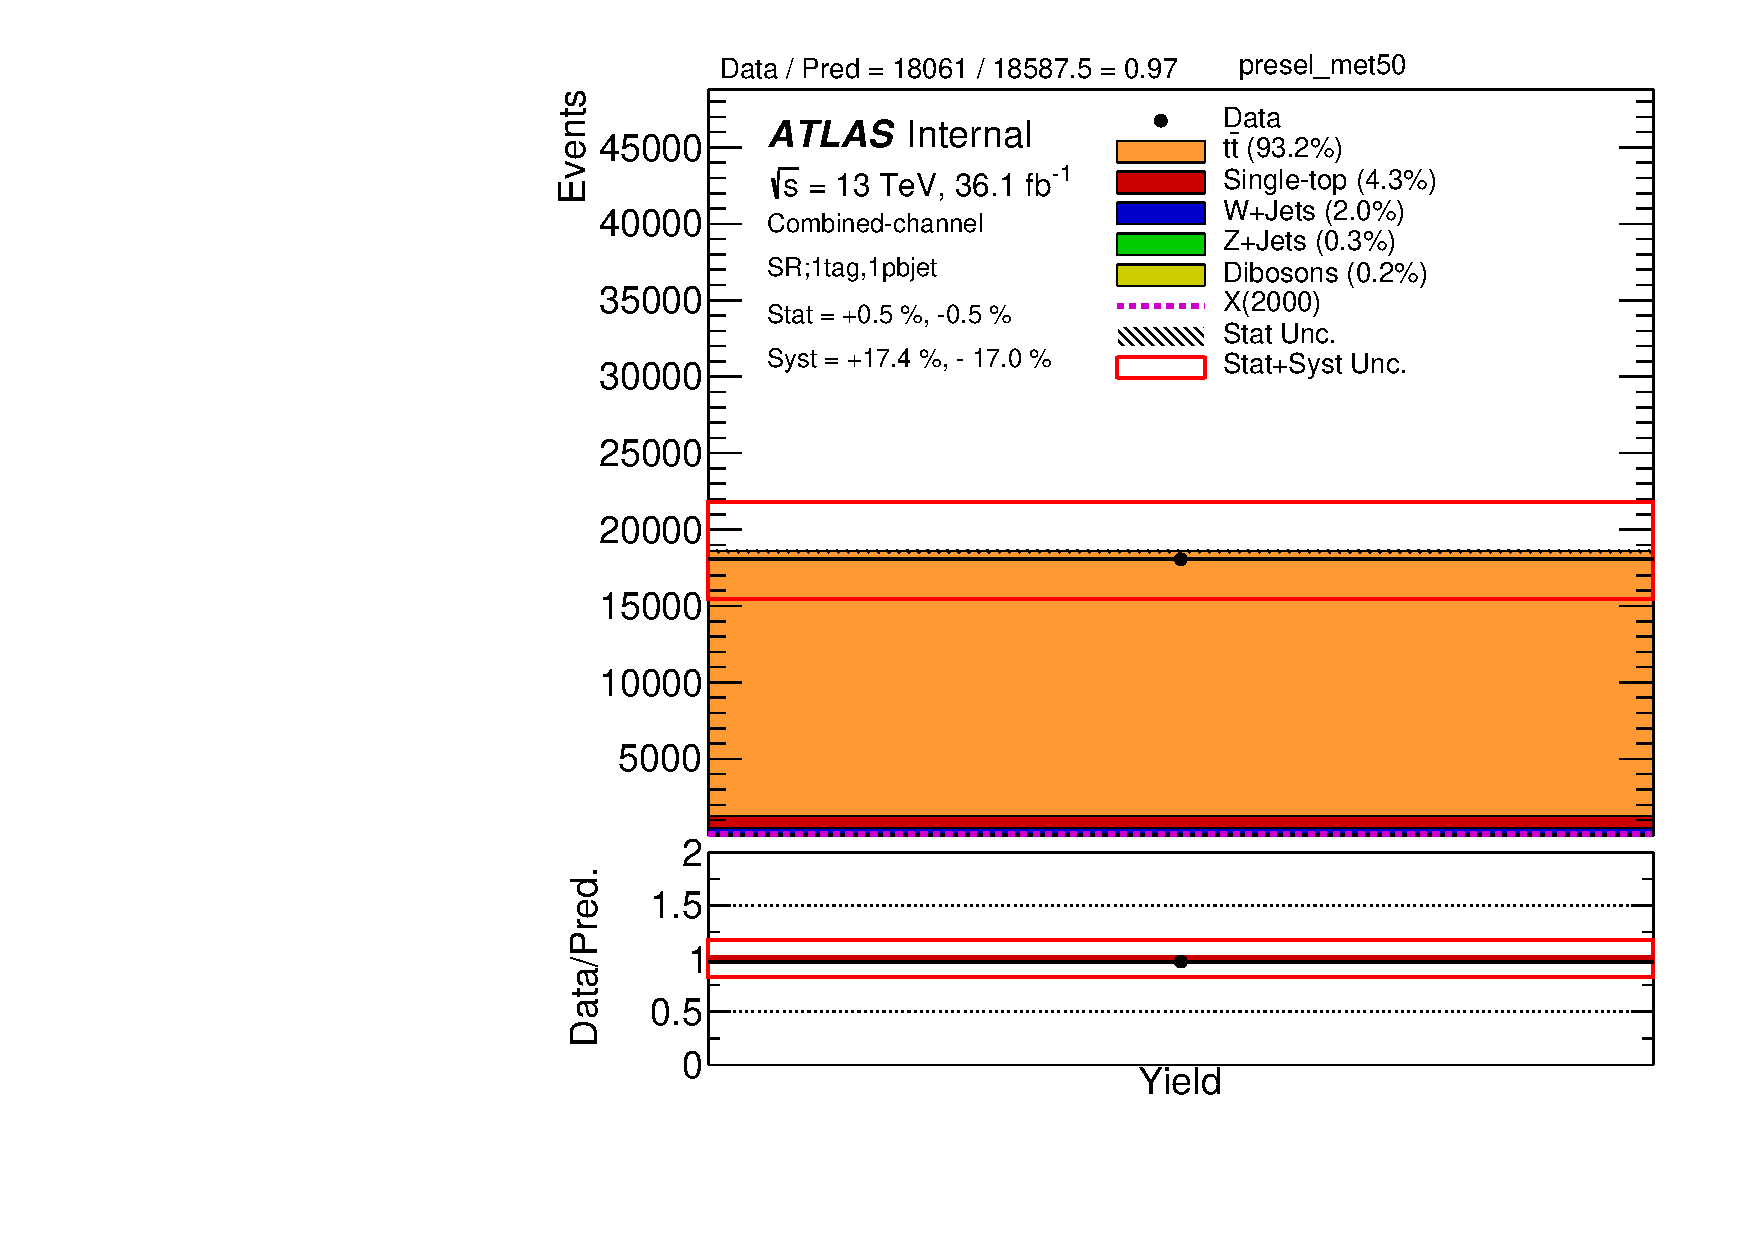
\includegraphics[scale=0.33]{./figures/boosted/Plot1tag1pbjet/DataMC_1tag_1pbjet_SR_lepton_presel_met50_neventsweighted} \\
\caption{Predicted and observed yield of events in the 1tag,1pbjet signal region.}
\label{fig:boosted_SR_1tag_1pbjet_normplot}
\end{center}
\end{figure}

\begin{figure}[!htbp]
\begin{center}
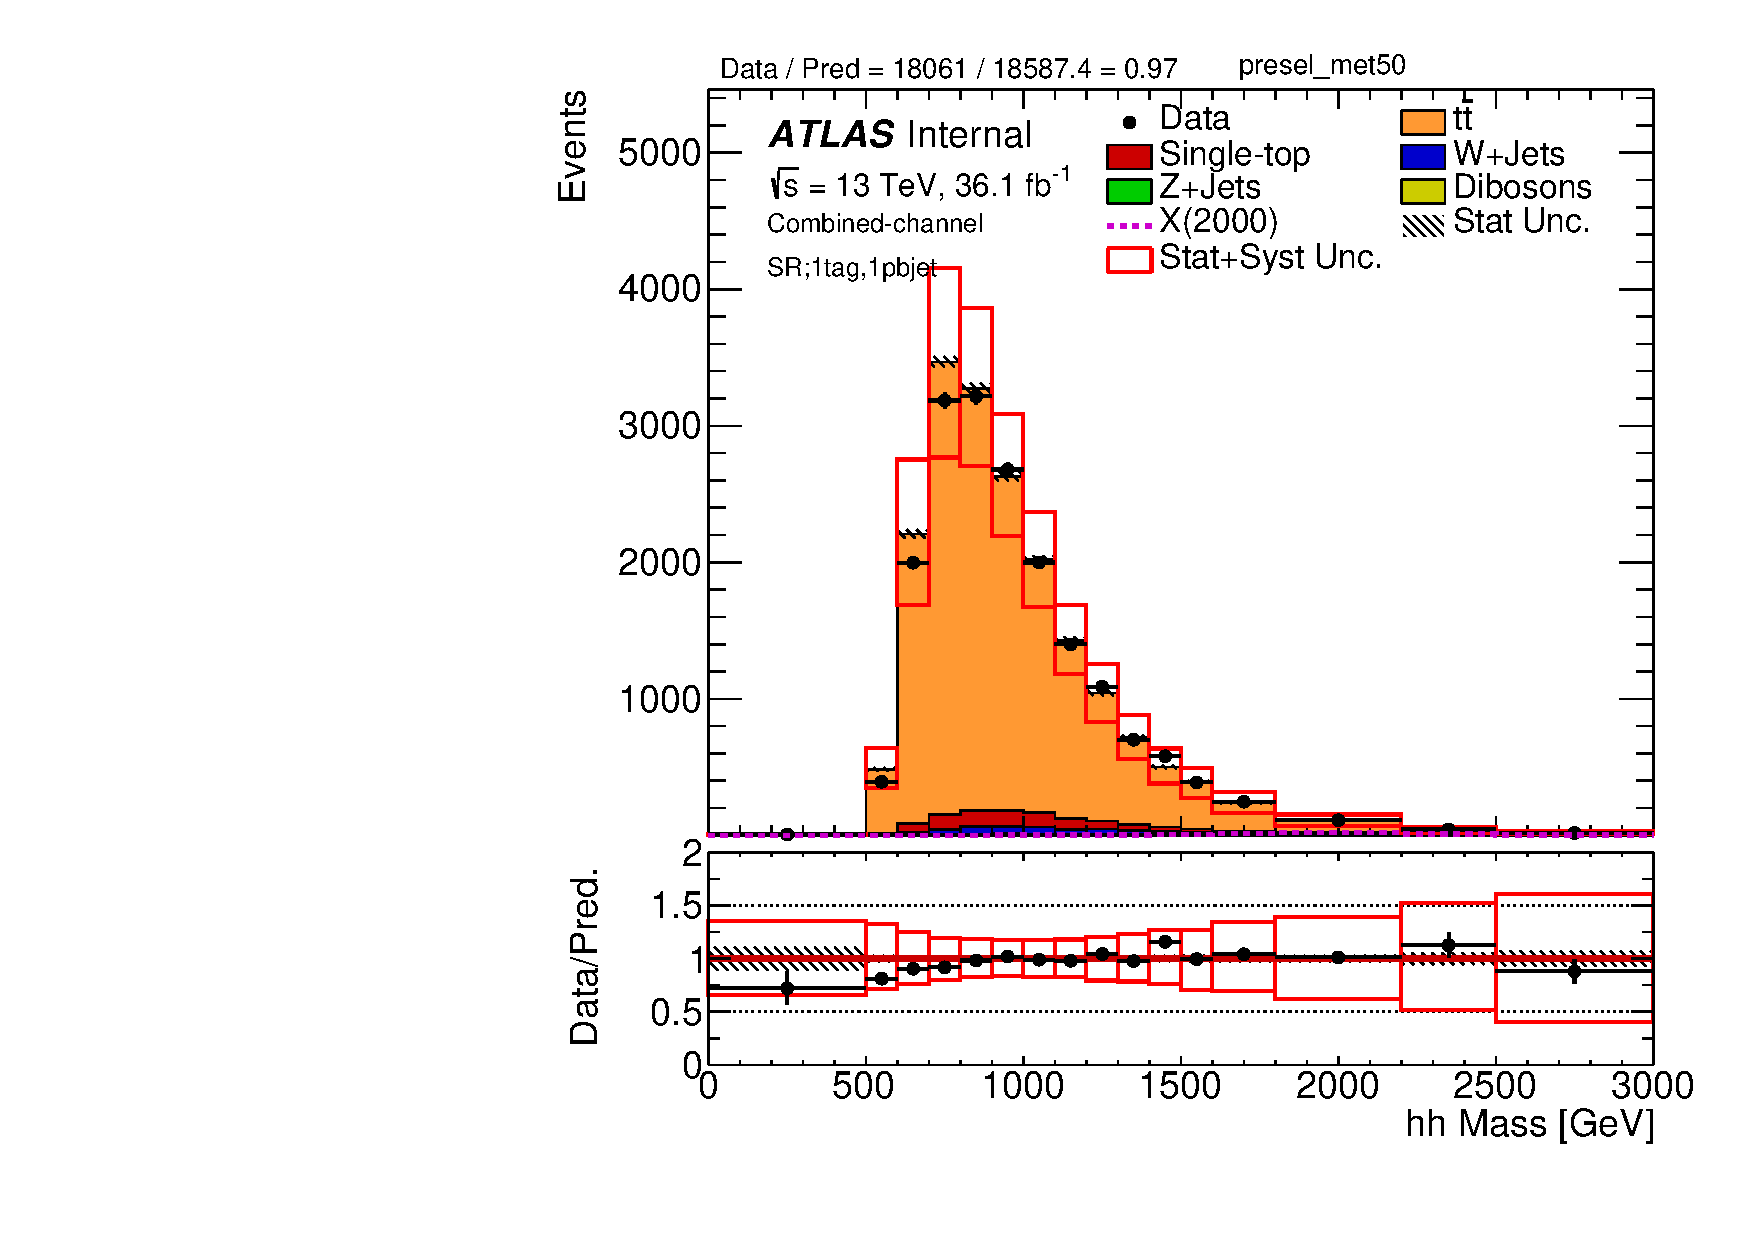
\includegraphics[scale=0.33]{./figures/boosted/Plot1tag1pbjet/DataMC_1tag_1pbjet_SR_lepton_presel_met50_hhMassRebin1}\\
\par\medskip
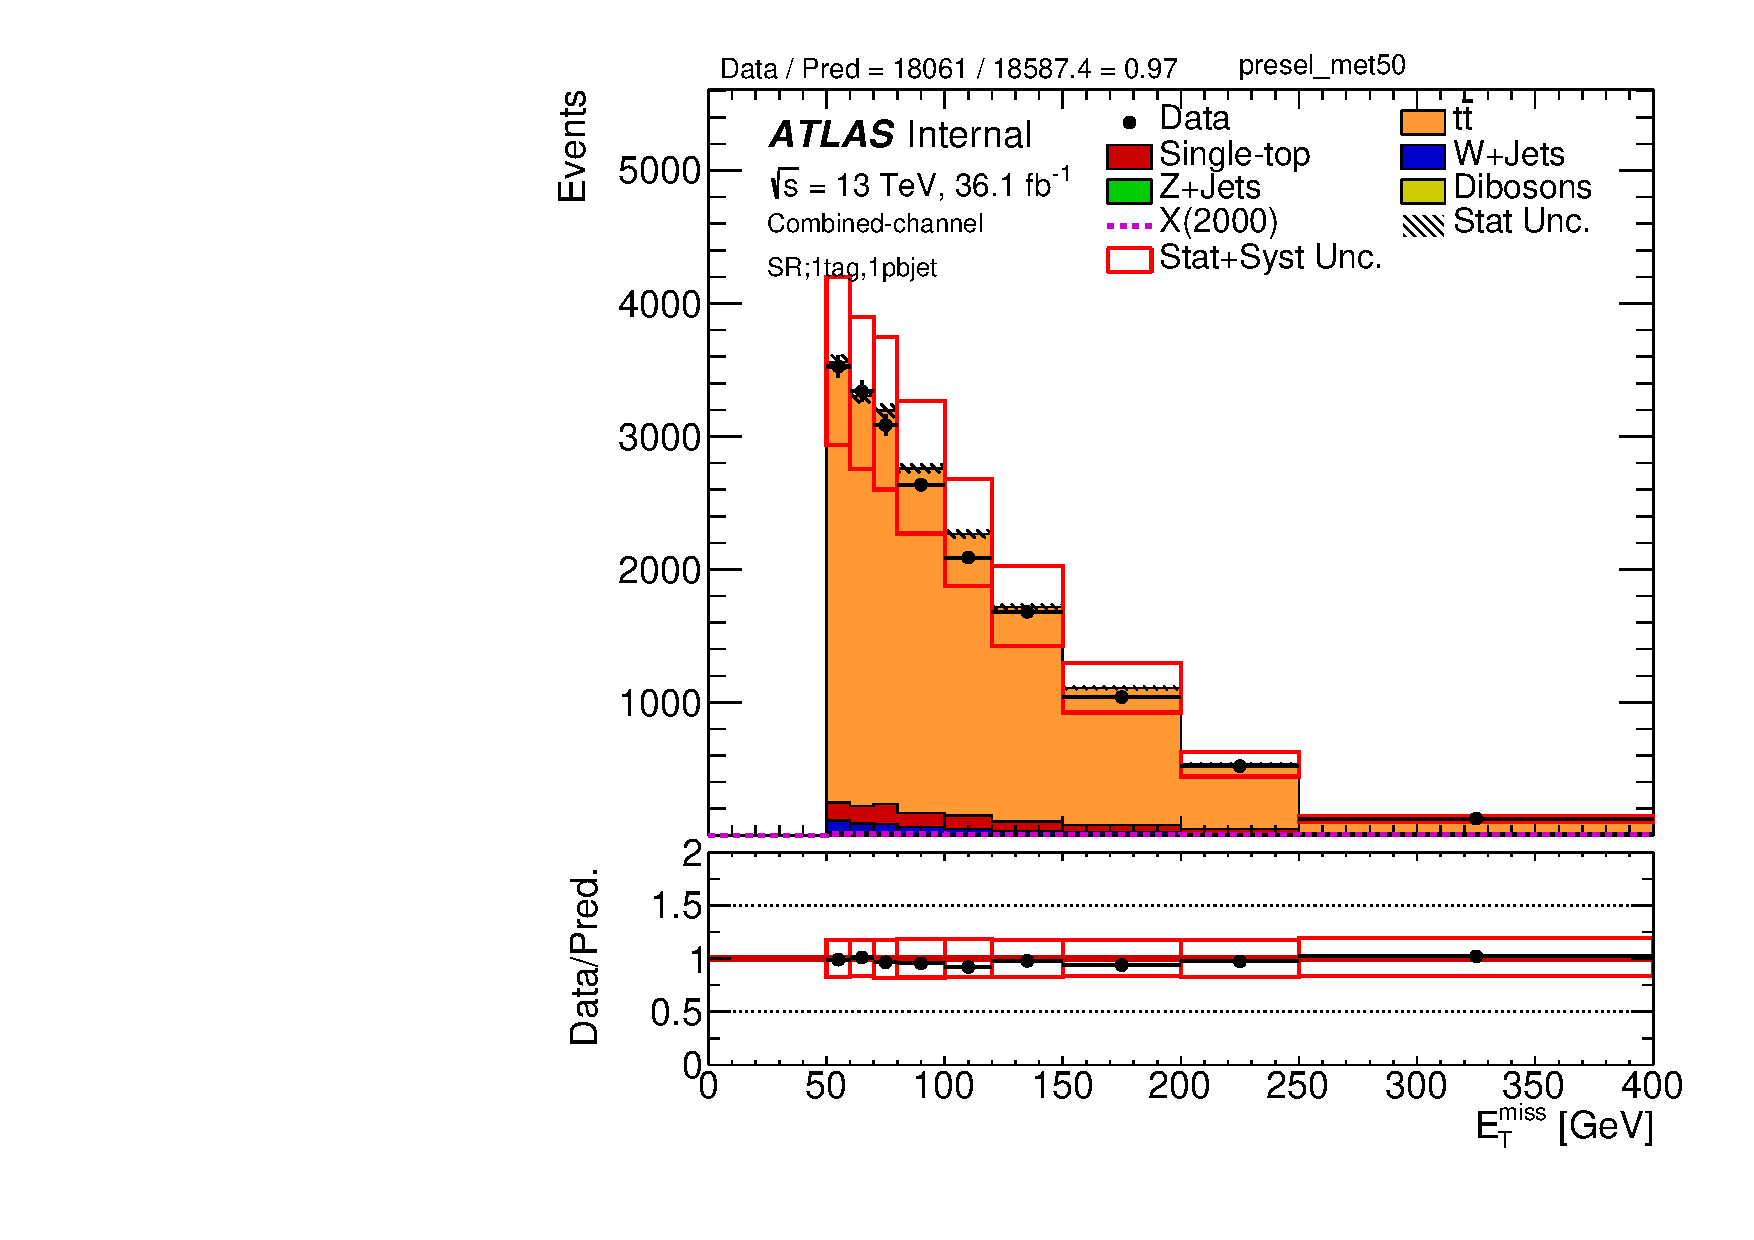
\includegraphics[scale=0.33]{./figures/boosted/Plot1tag1pbjet/DataMC_1tag_1pbjet_SR_lepton_presel_met50_MET}
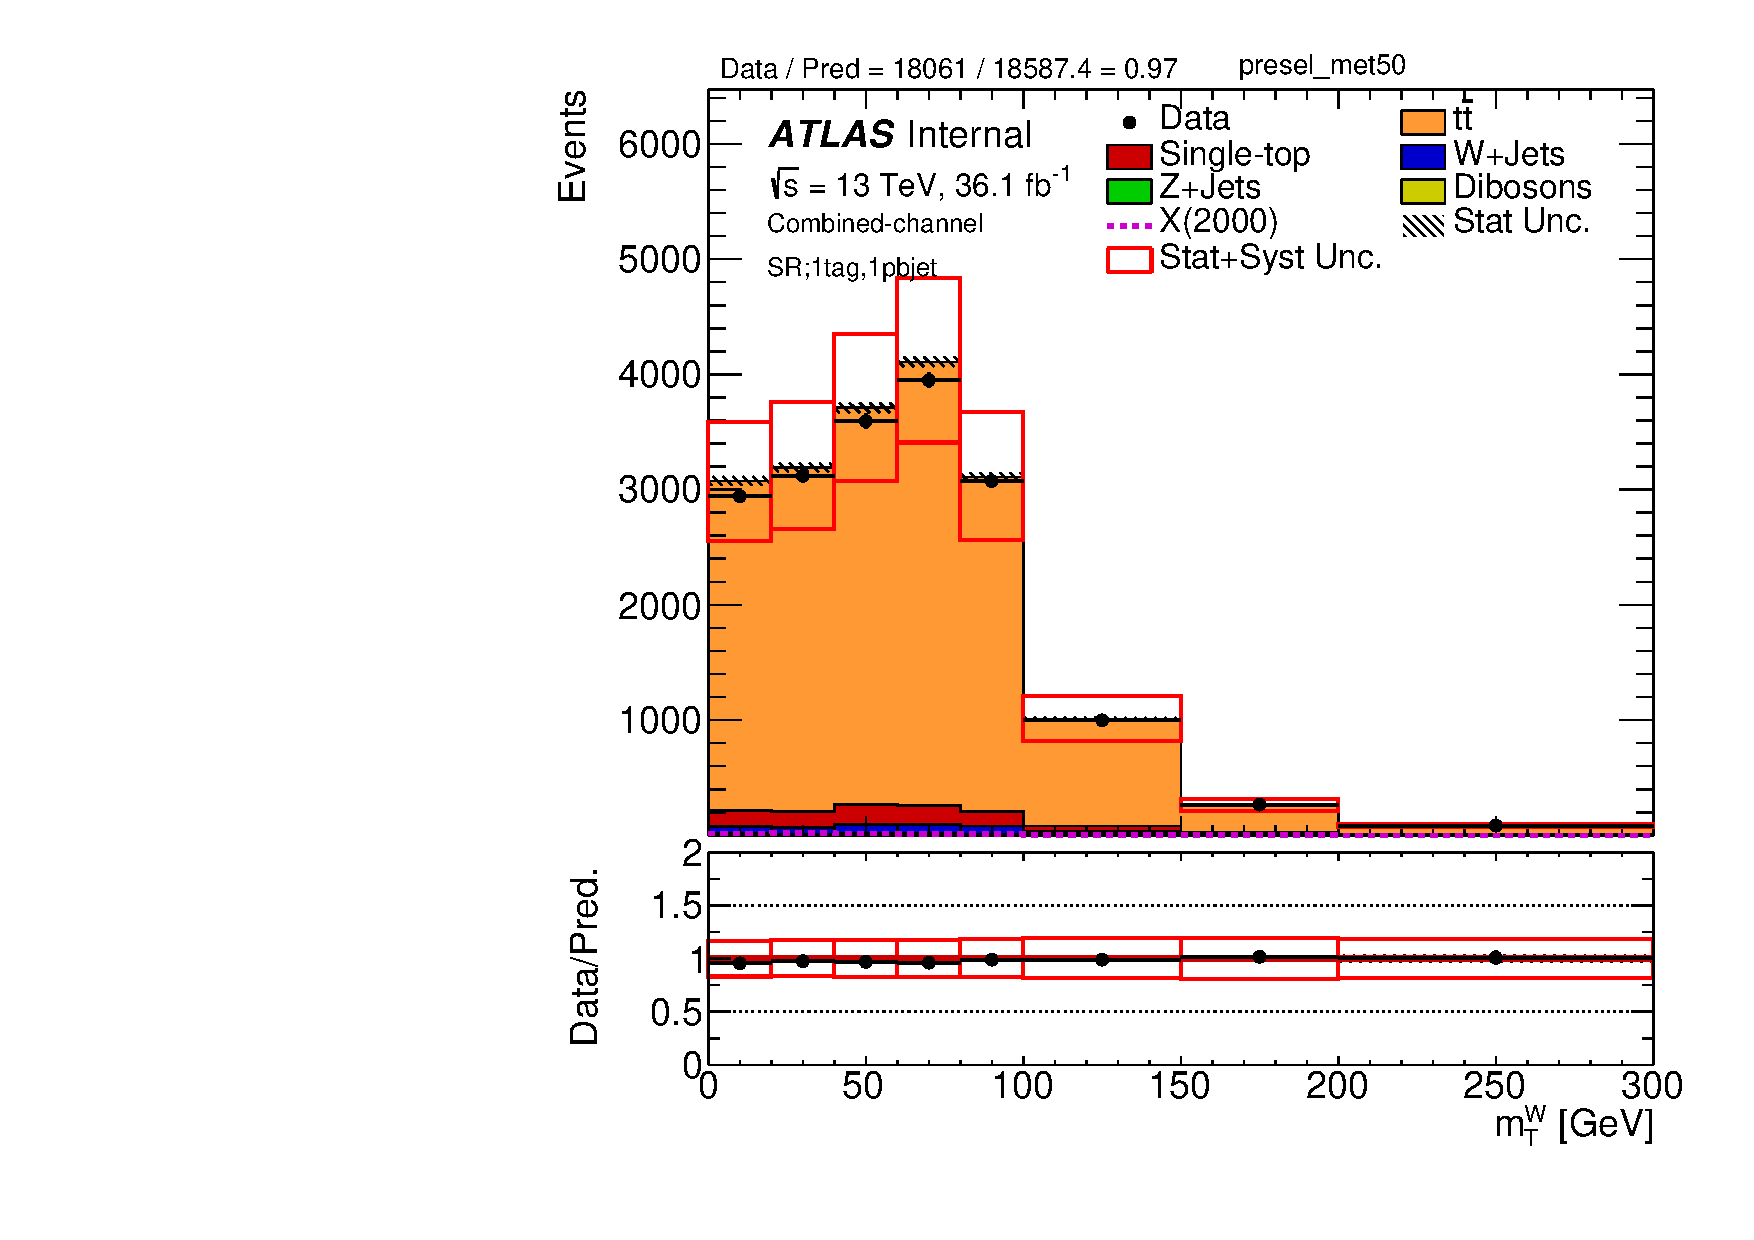
\includegraphics[scale=0.33]{./figures/boosted/Plot1tag1pbjet/DataMC_1tag_1pbjet_SR_lepton_presel_met50_WlepMtATLAS}
\caption{The invariant mass of the reconstructed di-Higgs (hh) system, \met and transverse mass of the $W \to l\nu$ system 
distributions of events in the 1tag,1pbjet signal region.}
\label{fig:boosted_SR_1tag_1pbjet_mainplots}
\end{center}
\end{figure}

\begin{figure}[!htbp]
\begin{center}
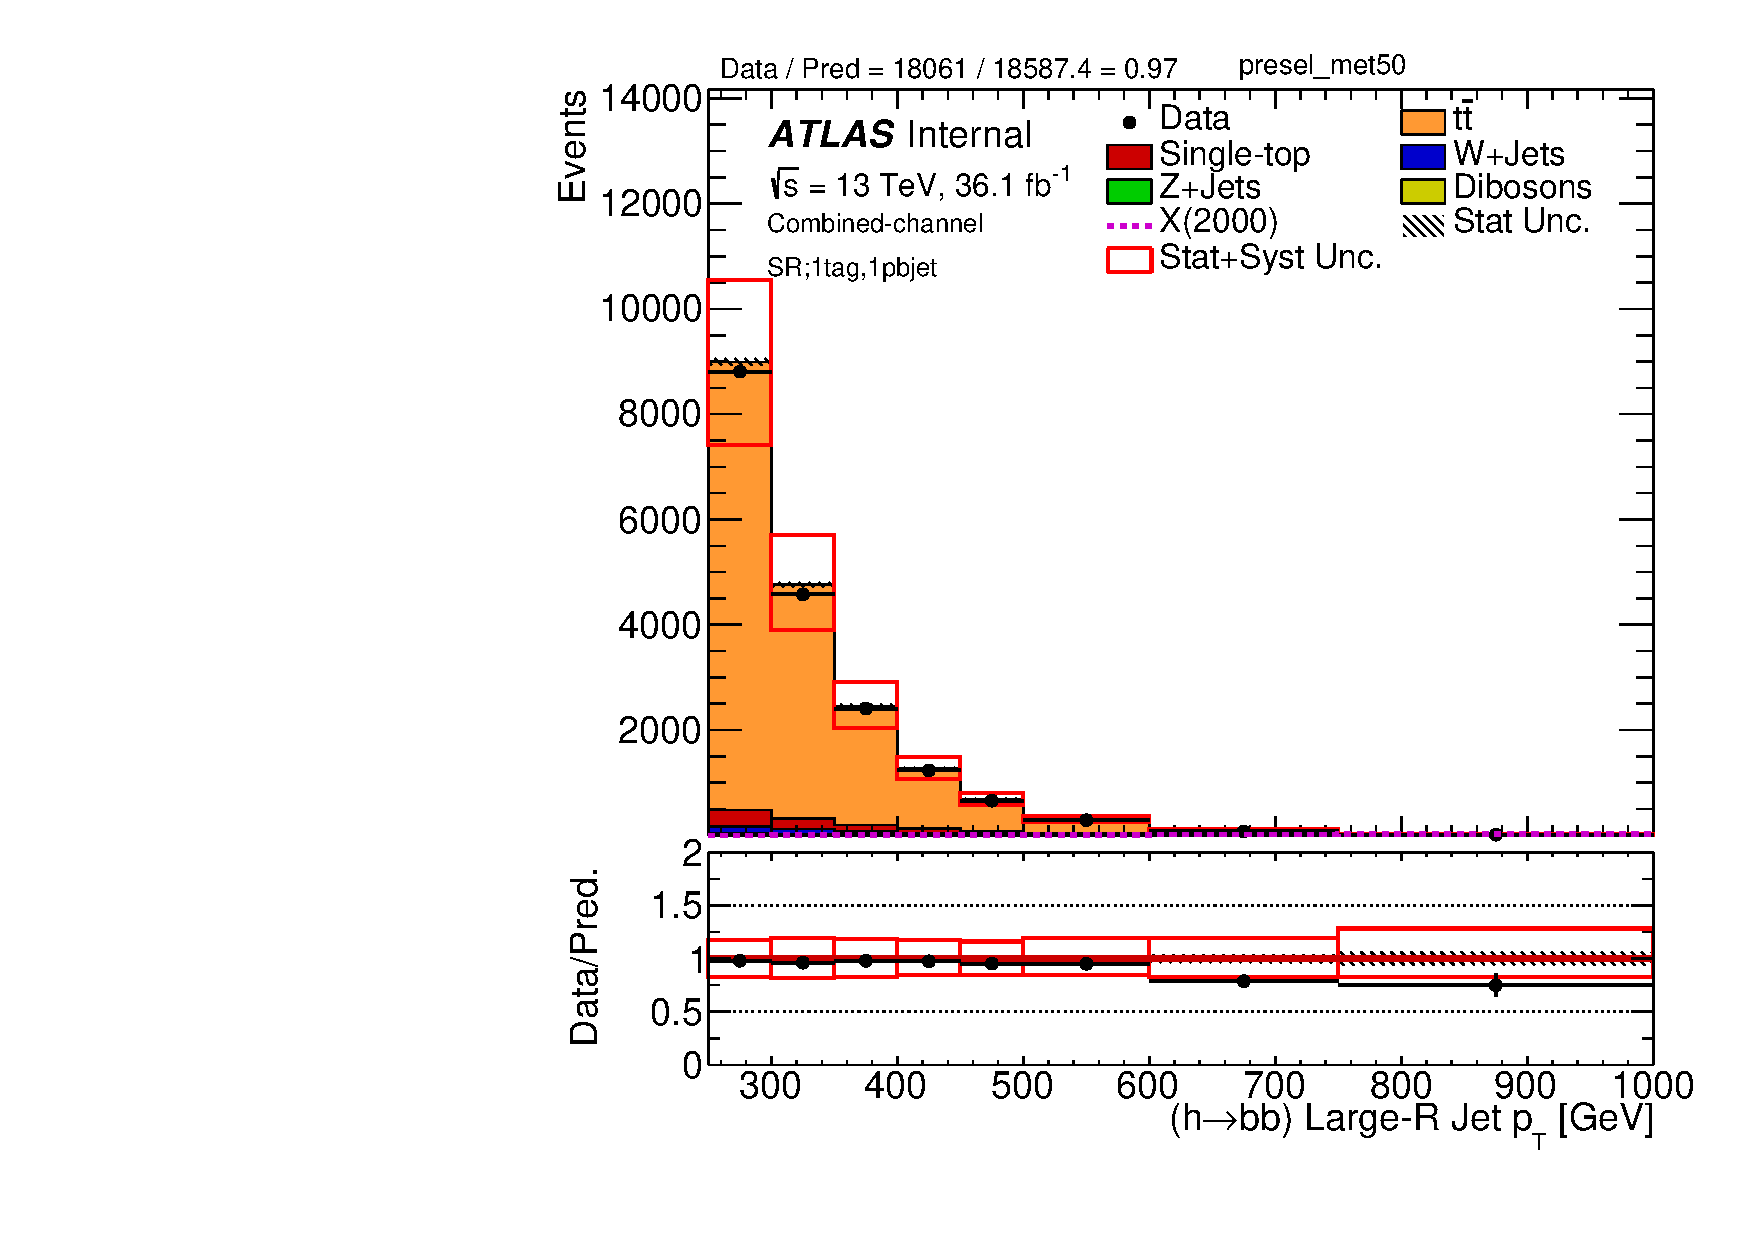
\includegraphics[scale=0.33]{./figures/boosted/Plot1tag1pbjet/DataMC_1tag_1pbjet_SR_lepton_presel_met50_HbbPt}
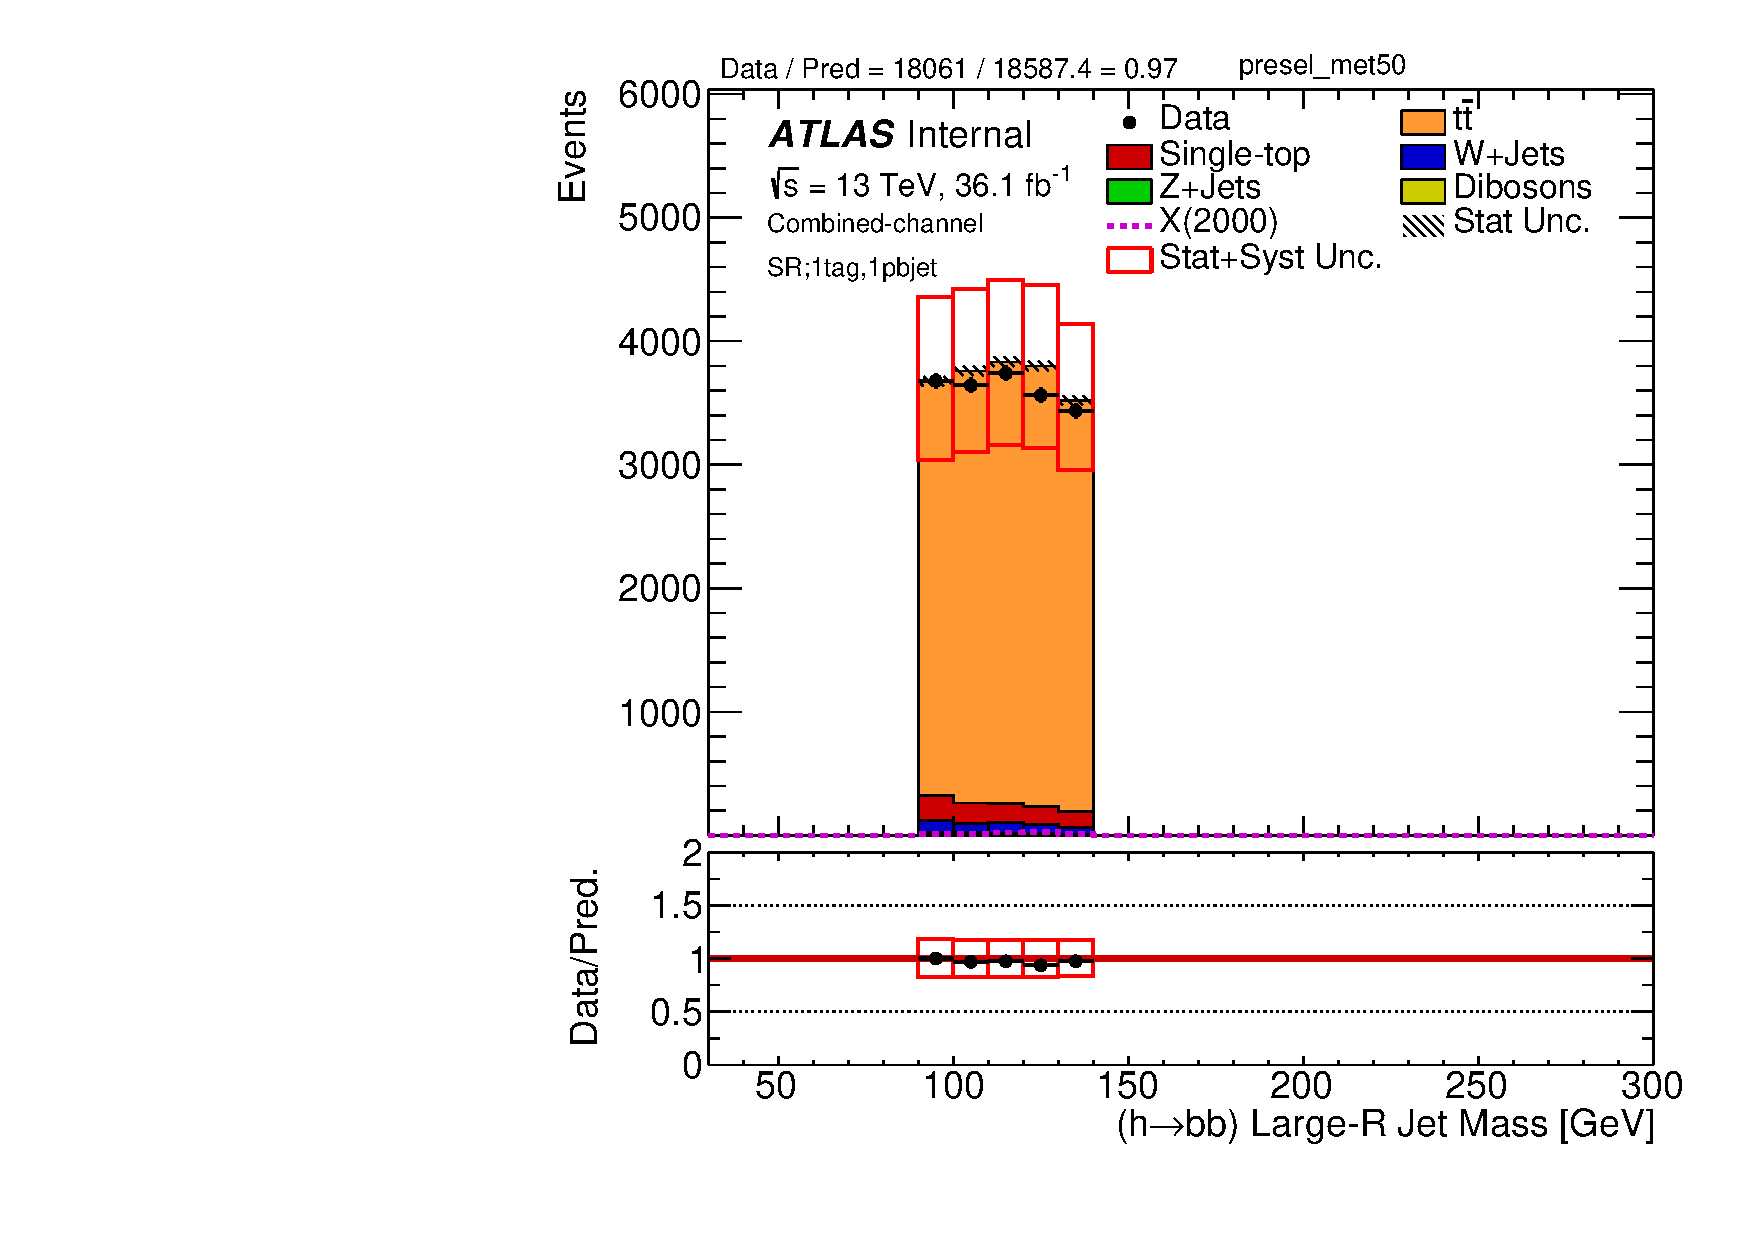
\includegraphics[scale=0.33]{./figures/boosted/Plot1tag1pbjet/DataMC_1tag_1pbjet_SR_lepton_presel_met50_HbbMass}\\
\par\medskip
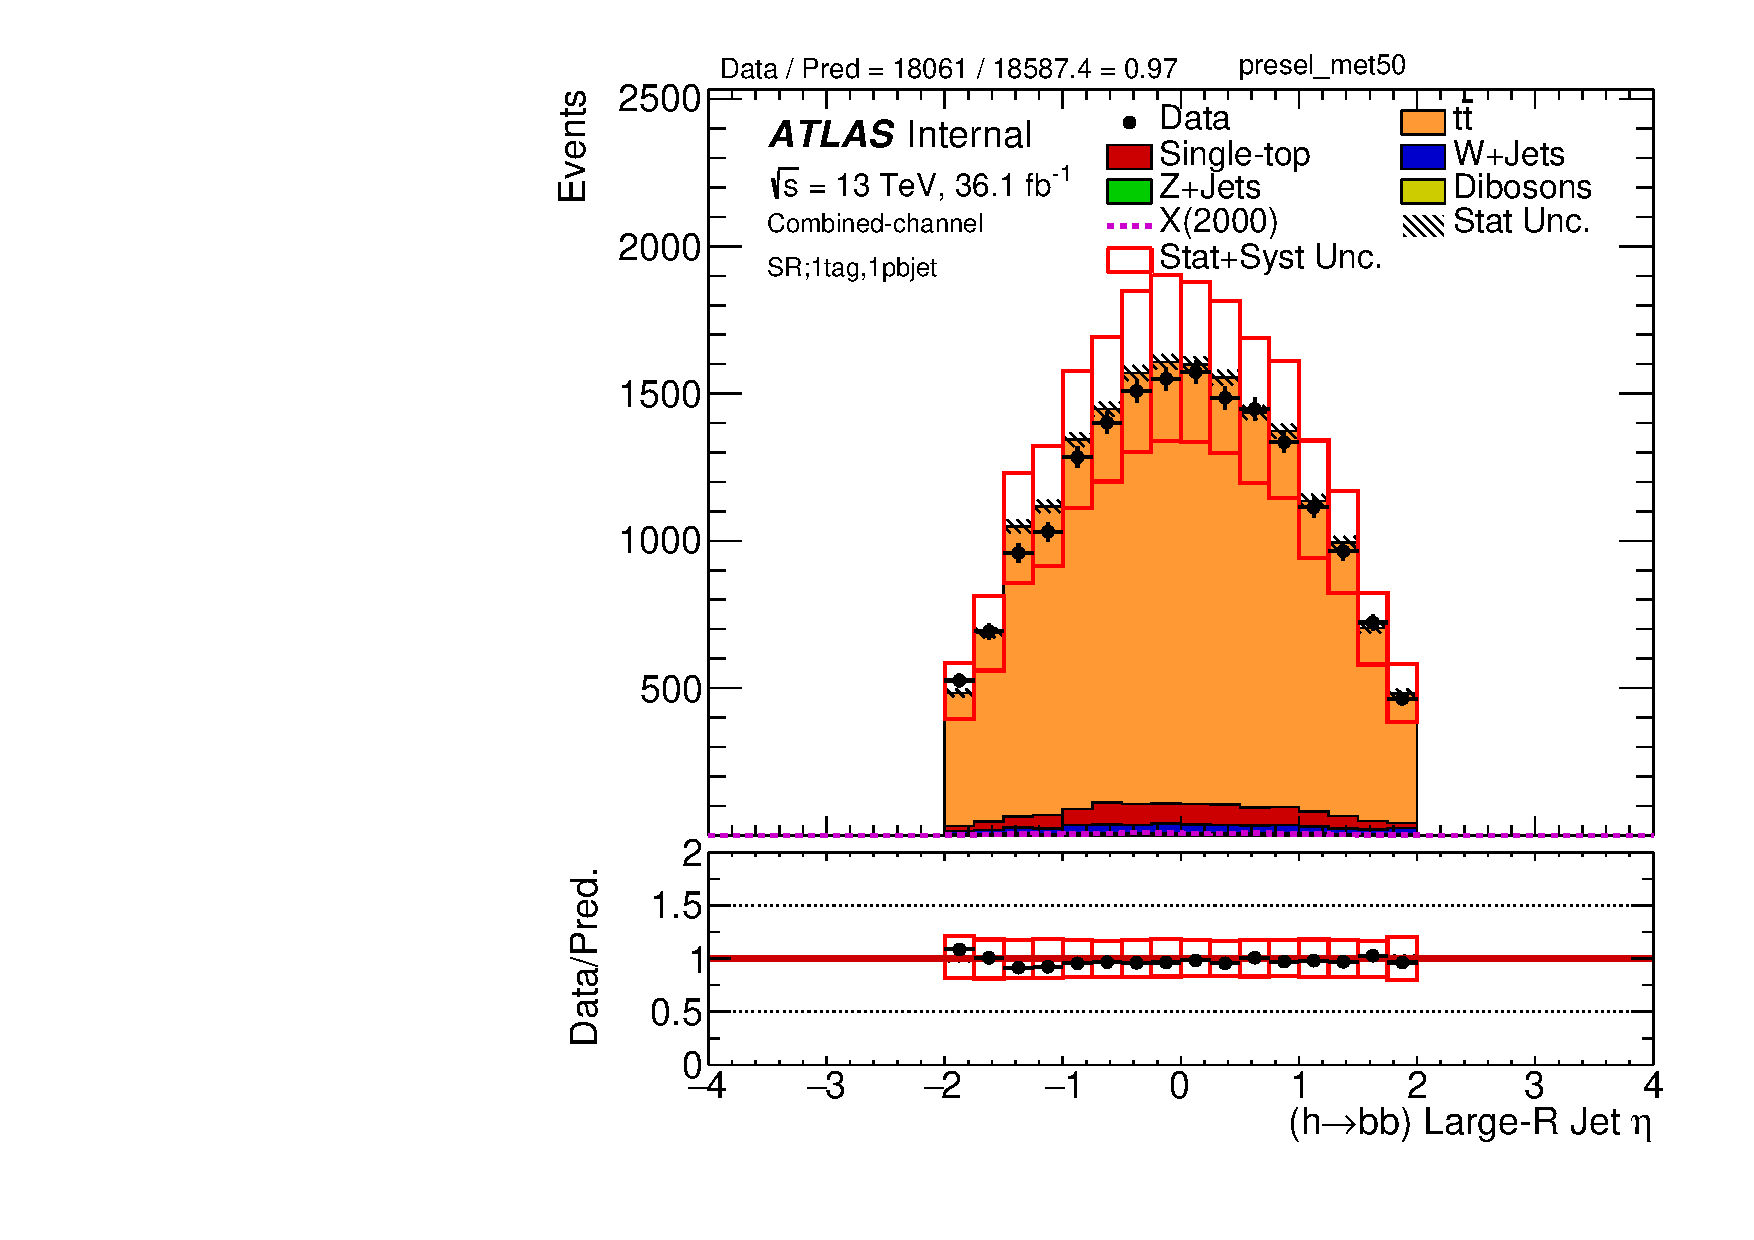
\includegraphics[scale=0.33]{./figures/boosted/Plot1tag1pbjet/DataMC_1tag_1pbjet_SR_lepton_presel_met50_HbbEta} 
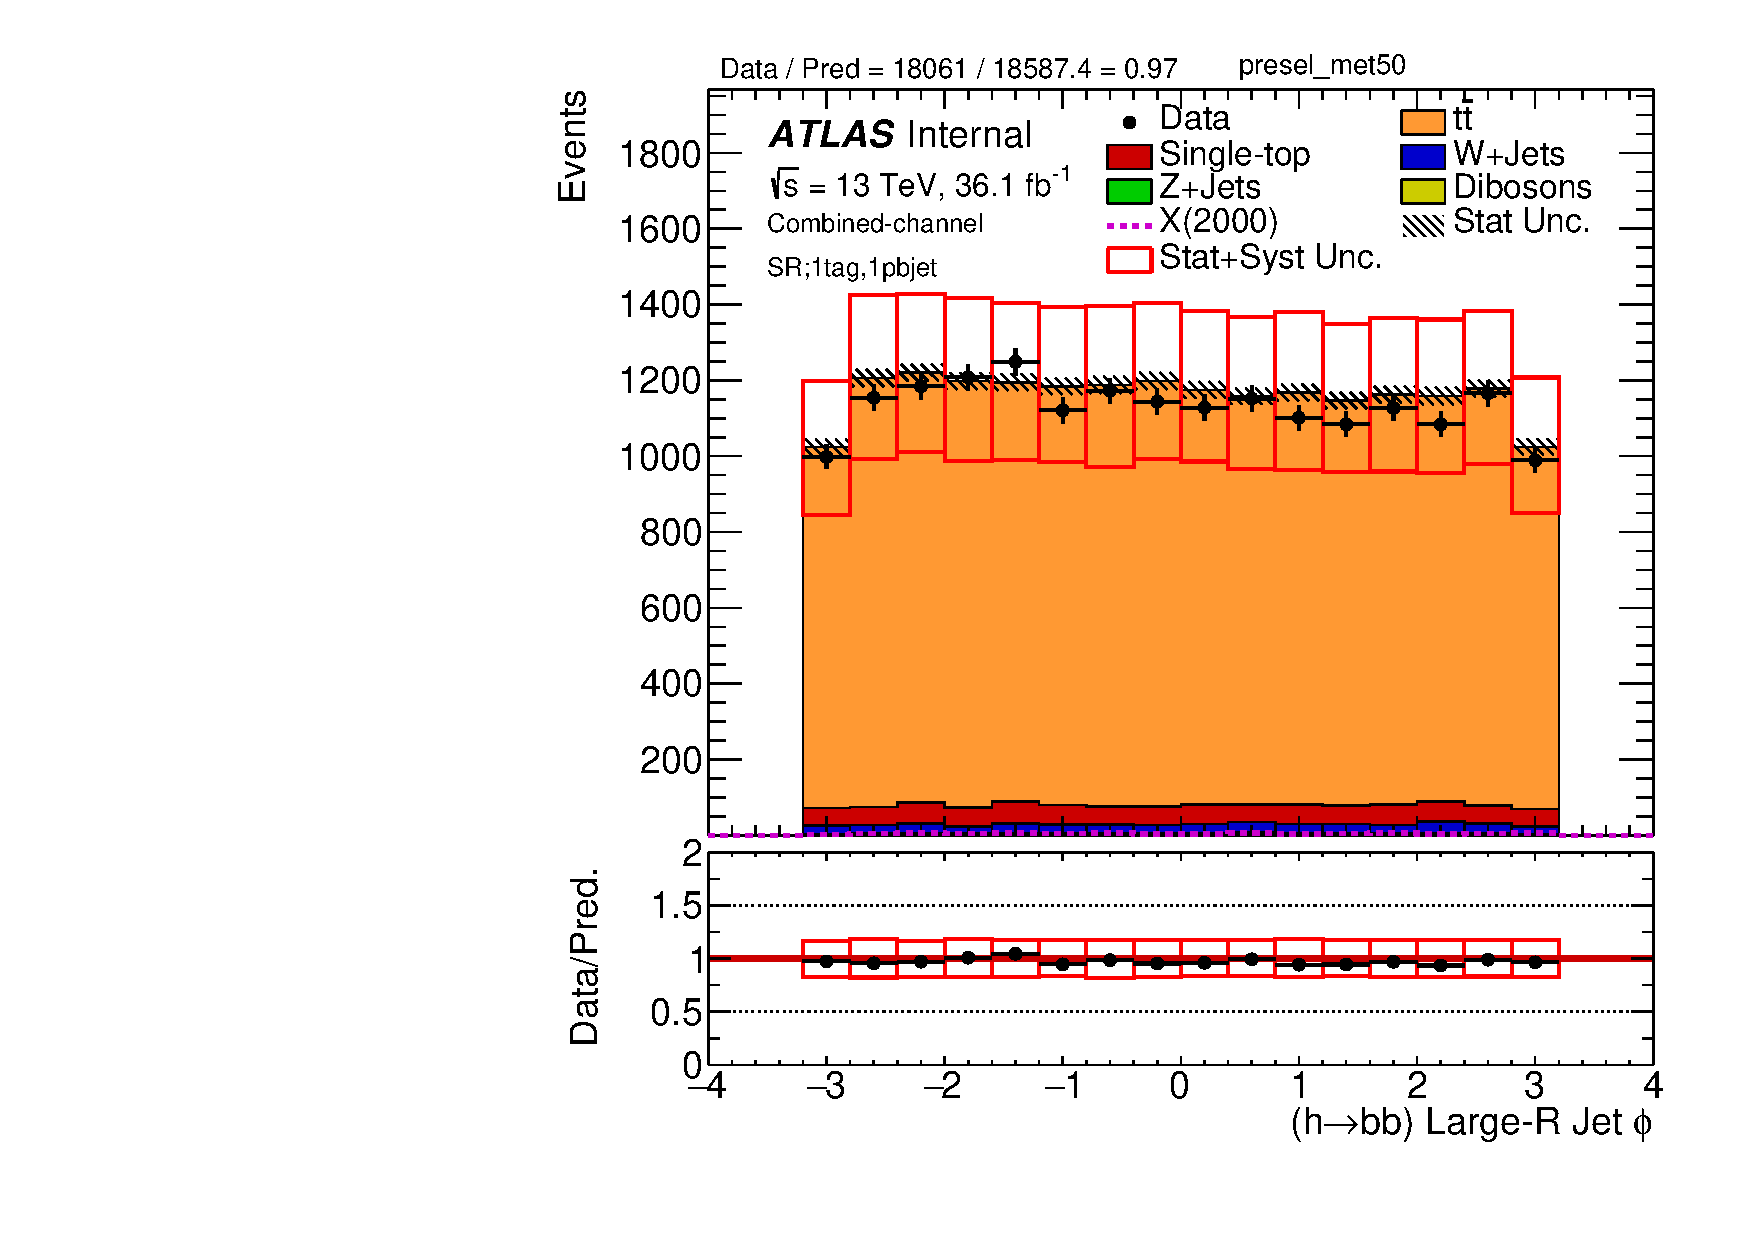
\includegraphics[scale=0.33]{./figures/boosted/Plot1tag1pbjet/DataMC_1tag_1pbjet_SR_lepton_presel_met50_HbbPhi} 
\caption{Kinematic distributions of the reconstructed large-$R$ jet in the 1tag,1pbjet signal region.}
\label{fig:boosted_SR_1tag_1pbjet_largerjet}
\end{center}
\end{figure}

% \begin{figure}[!h]
% \begin{center}
% 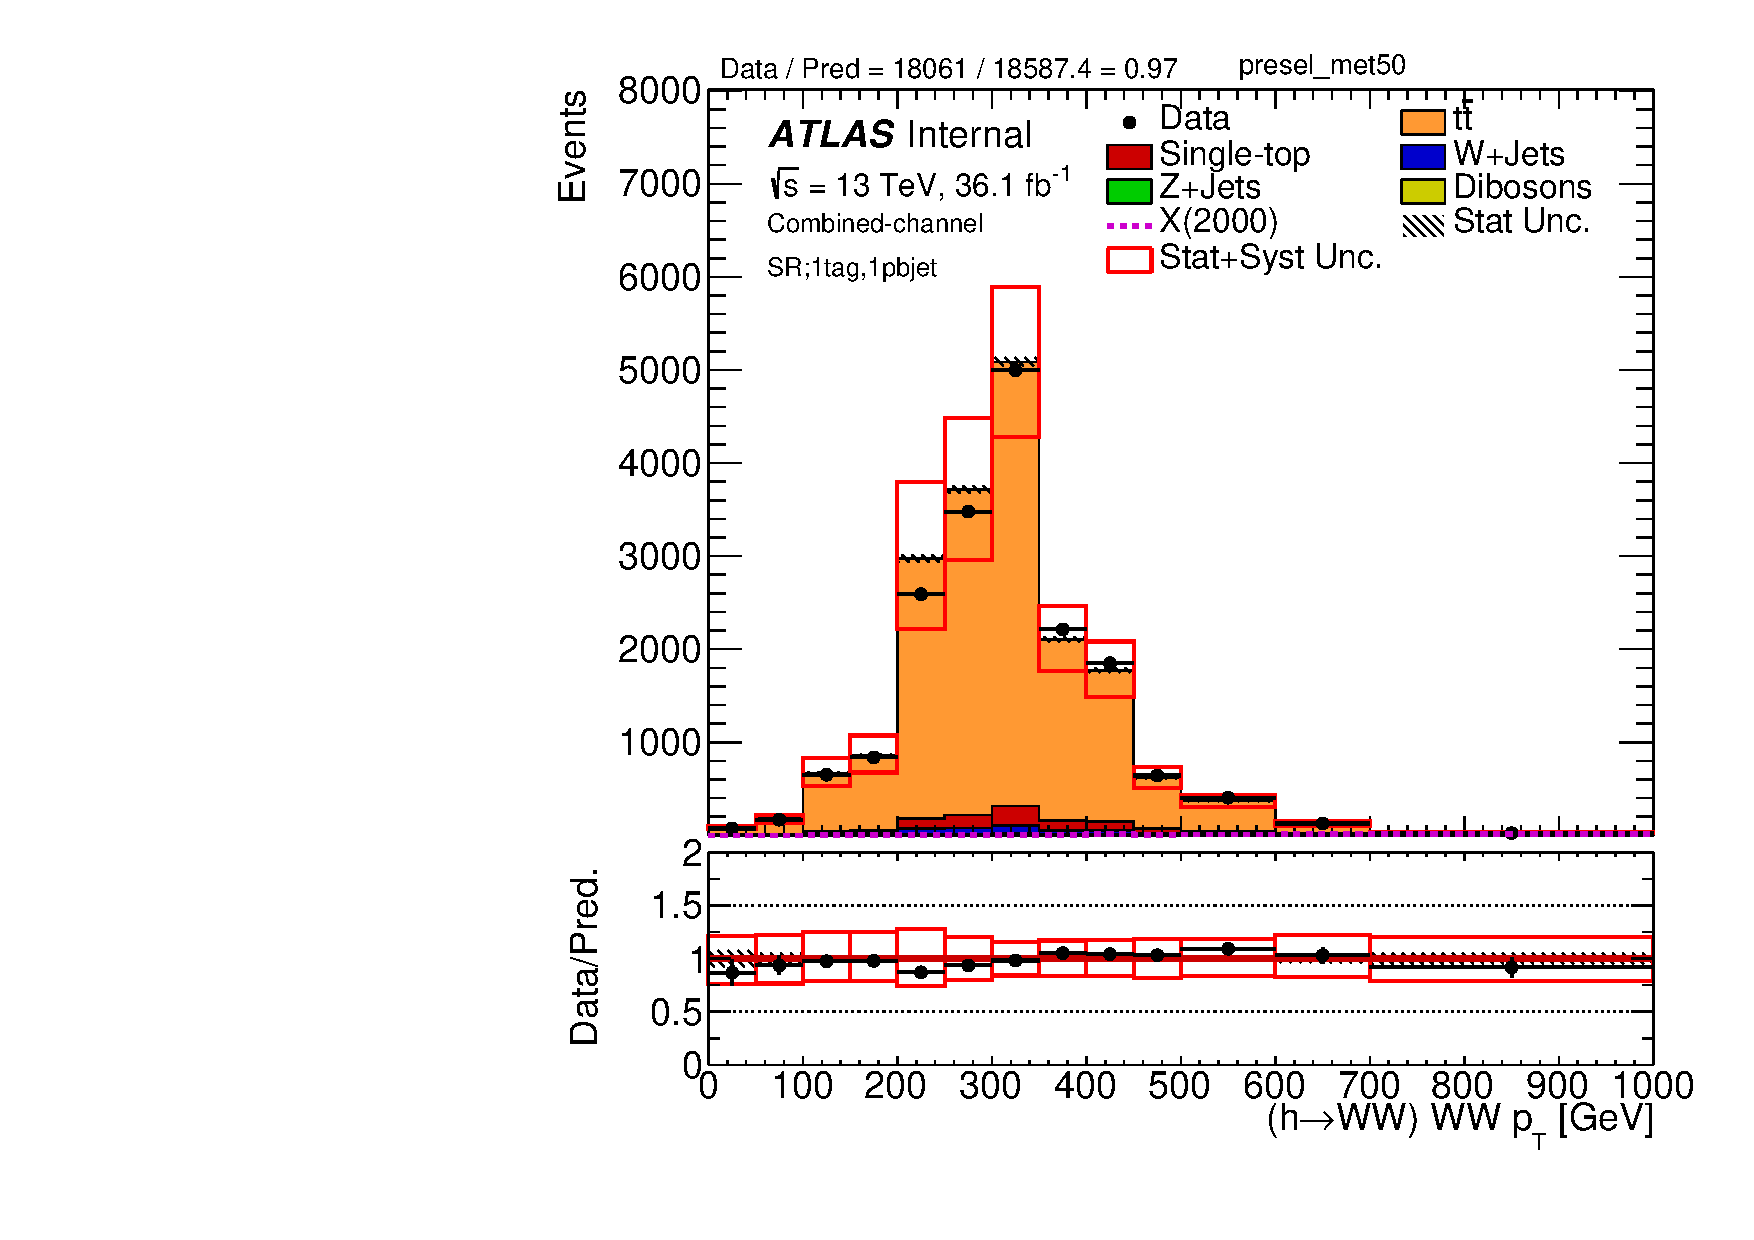
\includegraphics[scale=0.33]{./figures/boosted/Plot1tag1pbjet/DataMC_1tag_1pbjet_SR_lepton_presel_met50_WWPt}{fig:SR_1tag_1pbjet_hwwpt}{\pt} 
% 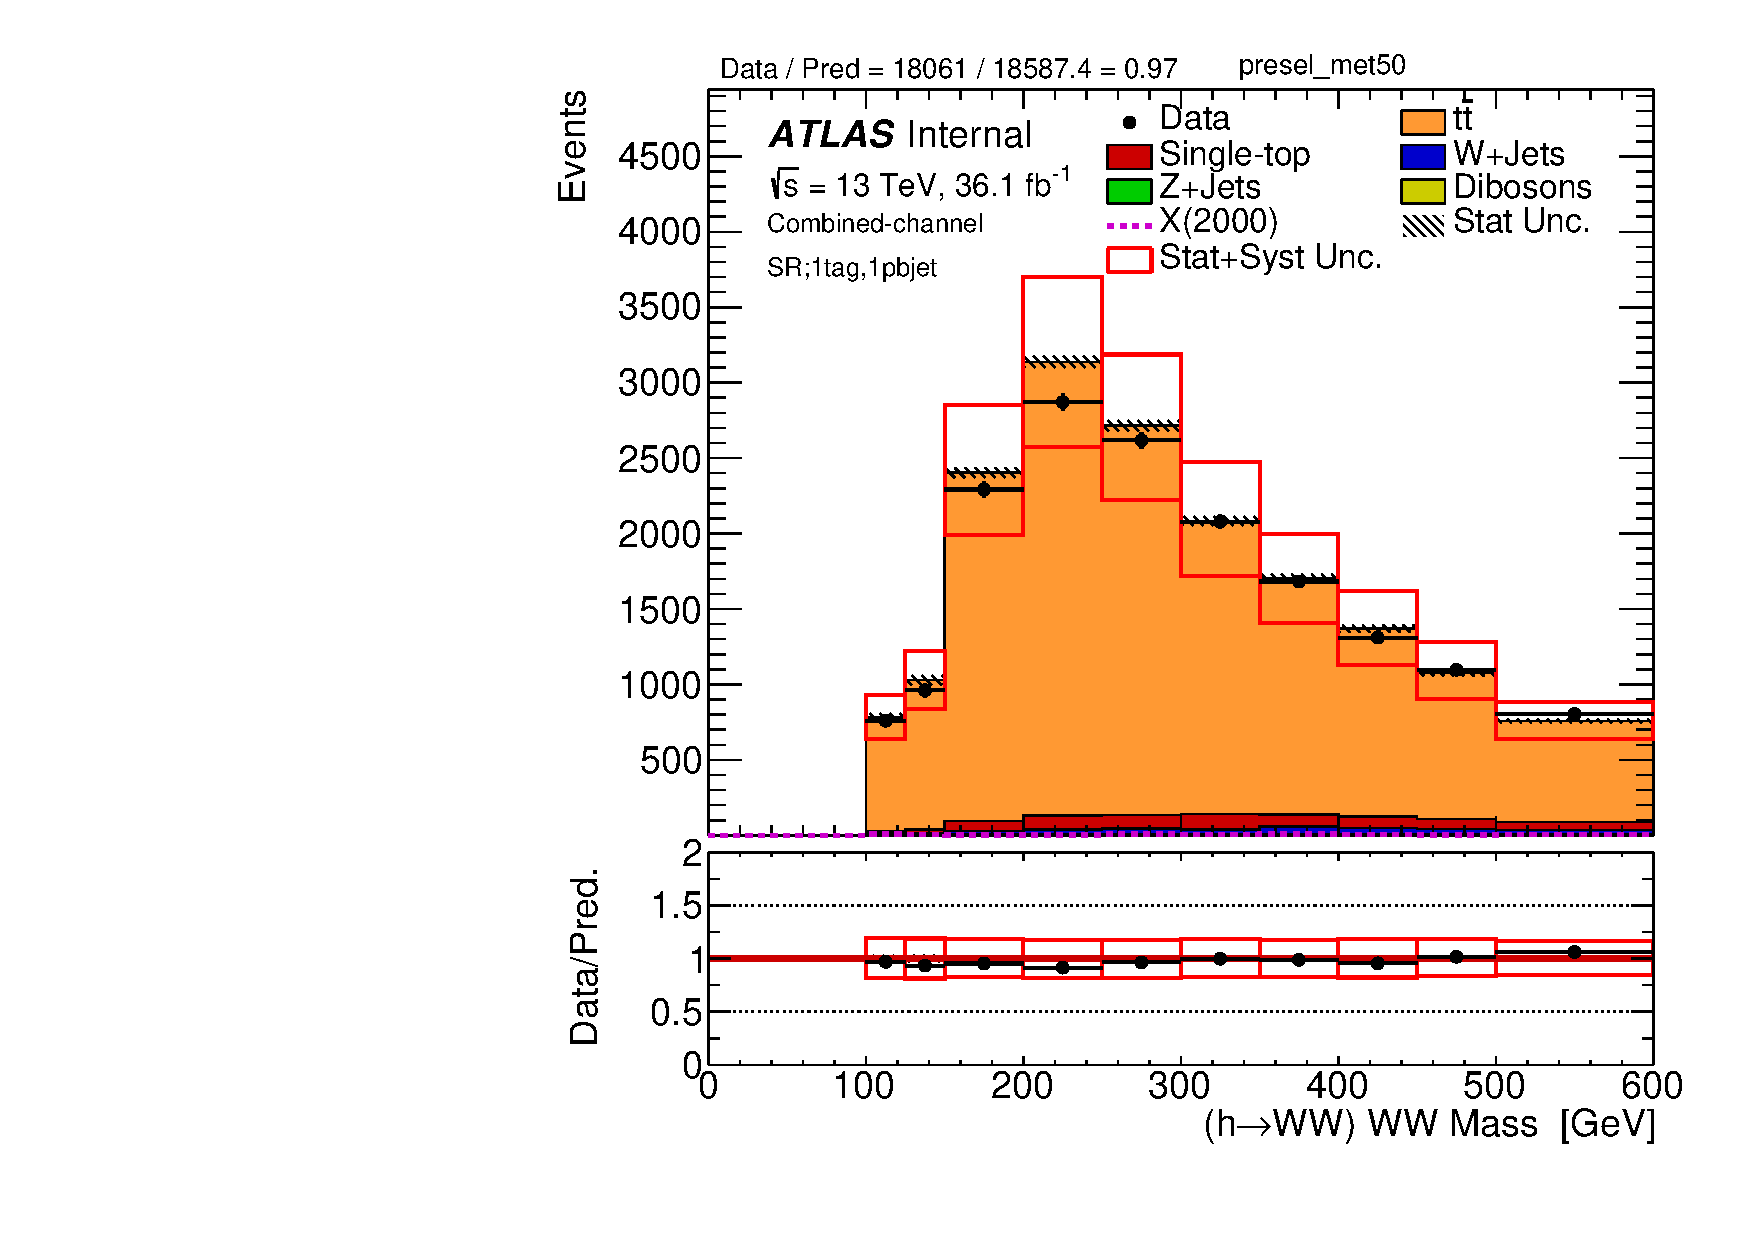
\includegraphics[scale=0.33]{./figures/boosted/Plot1tag1pbjet/DataMC_1tag_1pbjet_SR_lepton_presel_met50_WWMass}{fig:SR_1tag_1pbjet_hwwmass}{Mass} \\
% \par\medskip
% 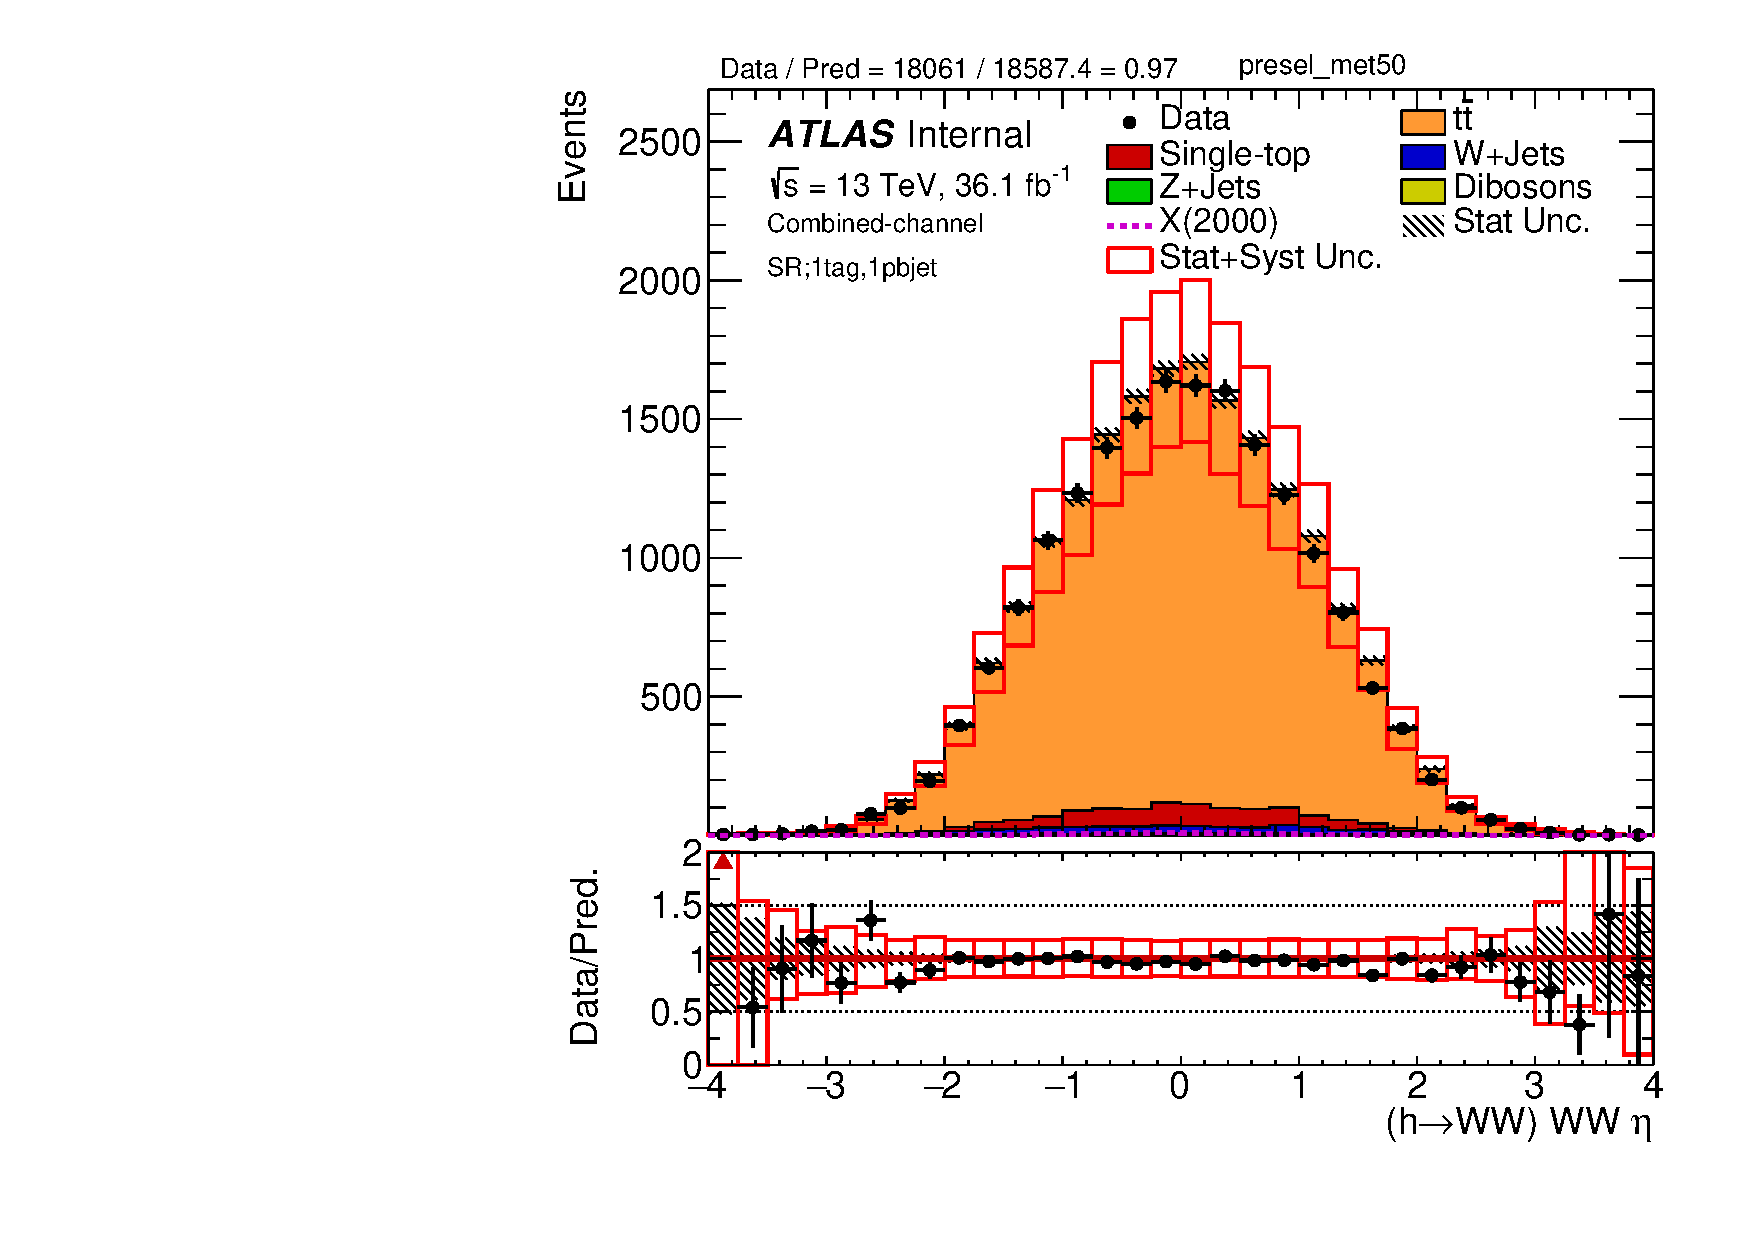
\includegraphics[scale=0.33]{./figures/boosted/Plot1tag1pbjet/DataMC_1tag_1pbjet_SR_lepton_presel_met50_WWEta}{fig:SR_1tag_1pbjet_hwweta}{$\eta$} 
% 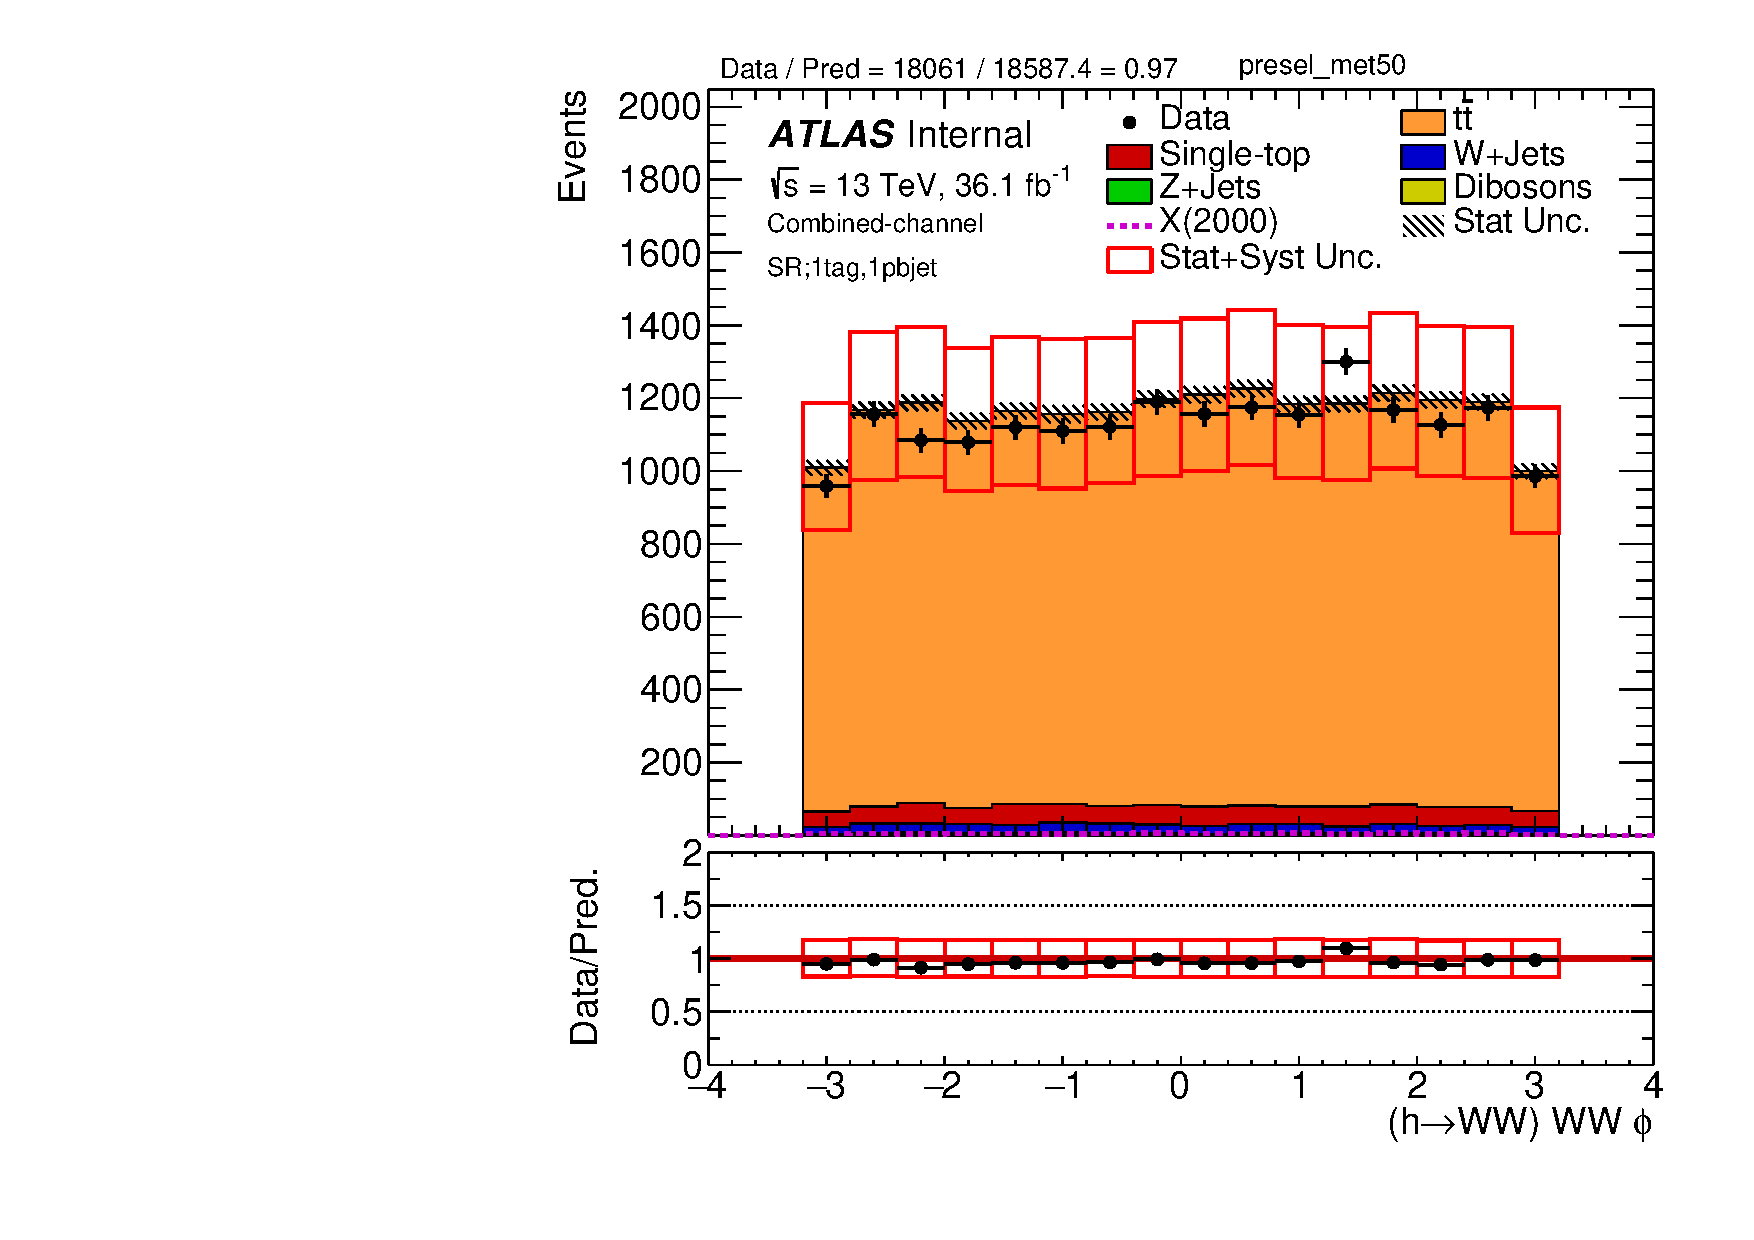
\includegraphics[scale=0.33]{./figures/boosted/Plot1tag1pbjet/DataMC_1tag_1pbjet_SR_lepton_presel_met50_WWPhi}{fig:SR_1tag_1pbjet_hwwphi}{$\phi$}
% \caption{Kinematic distributions of the reconstructed $h \to WW$ system in the 1tag,1pbjet signal region.
% All plots are prefit.}
% \label{fig:boosted_SR_1tag_1pbjet_wwsystem}
% \end{center}
% \end{figure}

% \begin{figure}[!h]
% \begin{center}
% 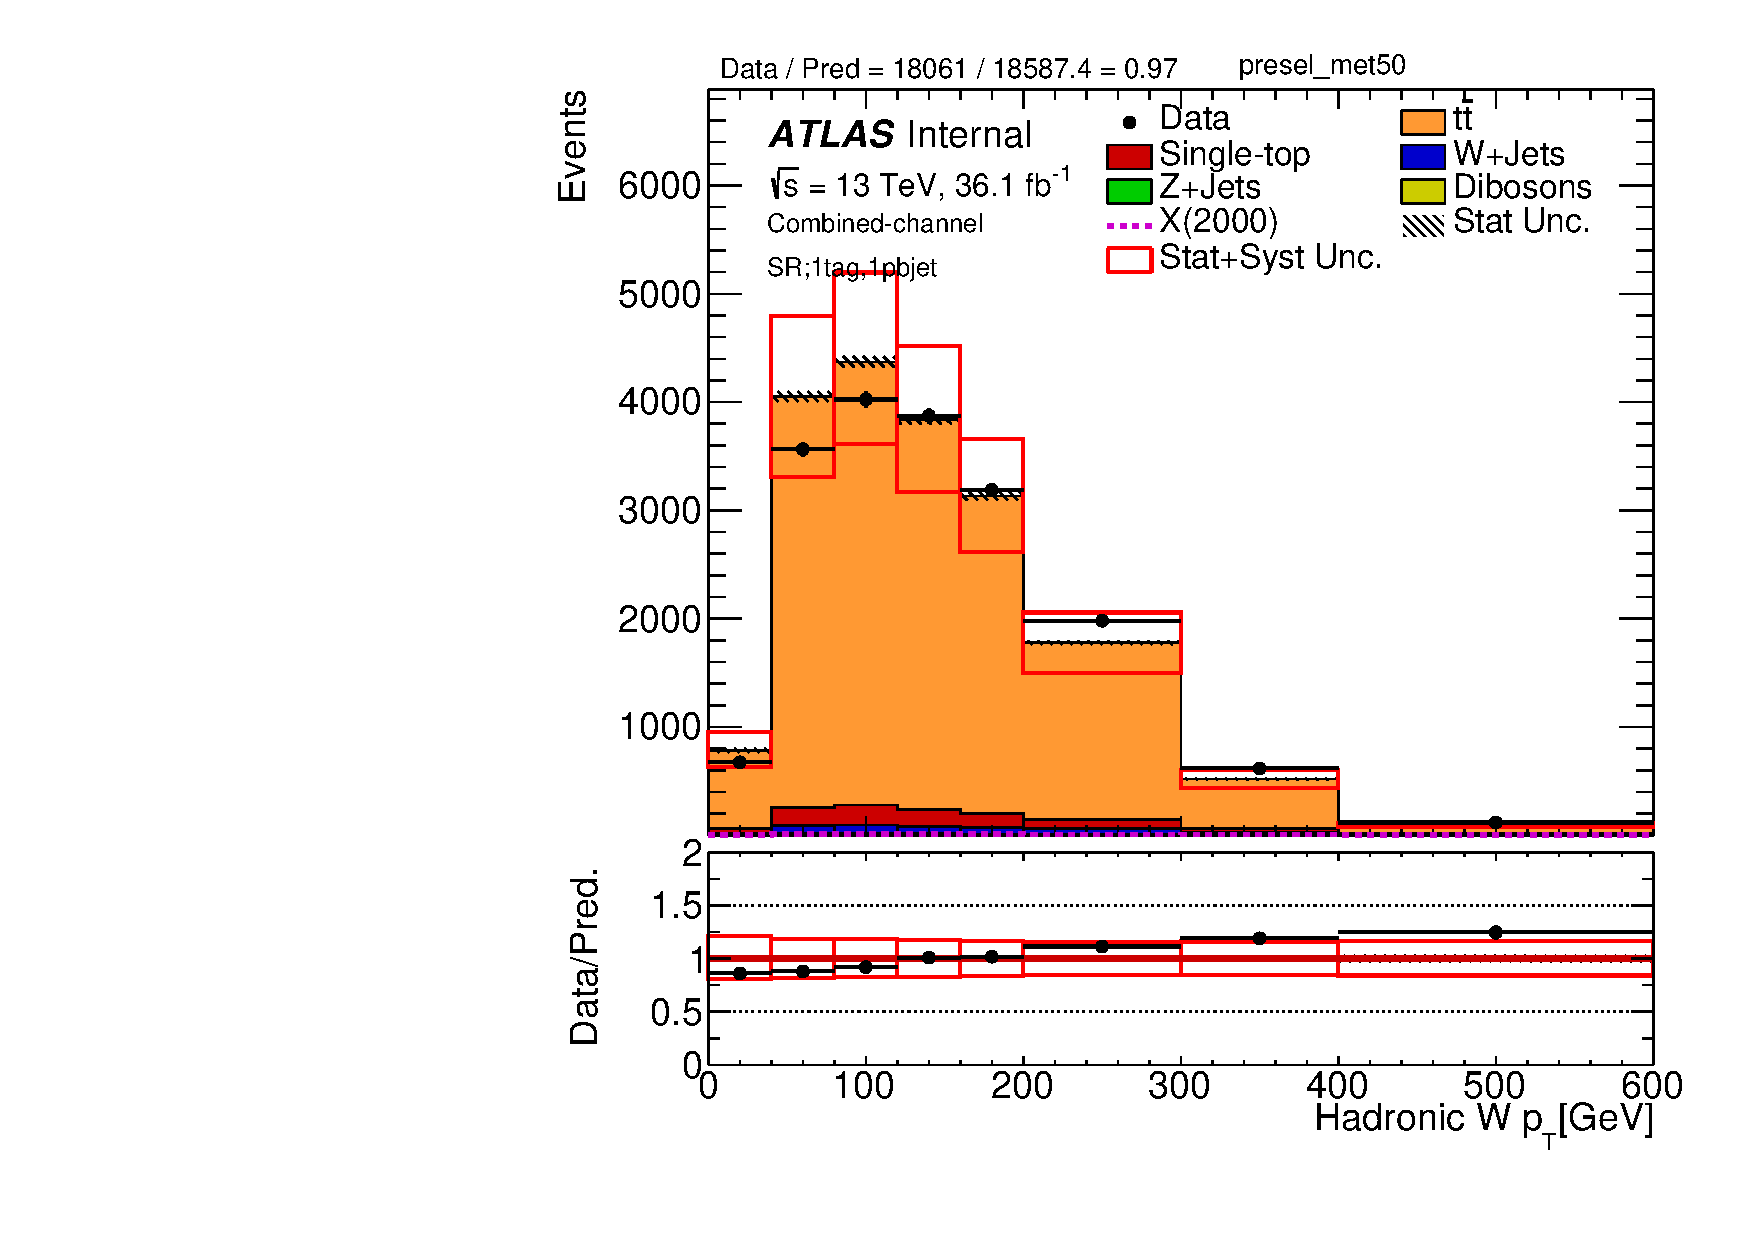
\includegraphics[scale=0.33]{./figures/boosted/Plot1tag1pbjet/DataMC_1tag_1pbjet_SR_lepton_presel_met50_WhadPt}{fig:SR_1tag_1pbjet_whadpt}{\pt} 
% 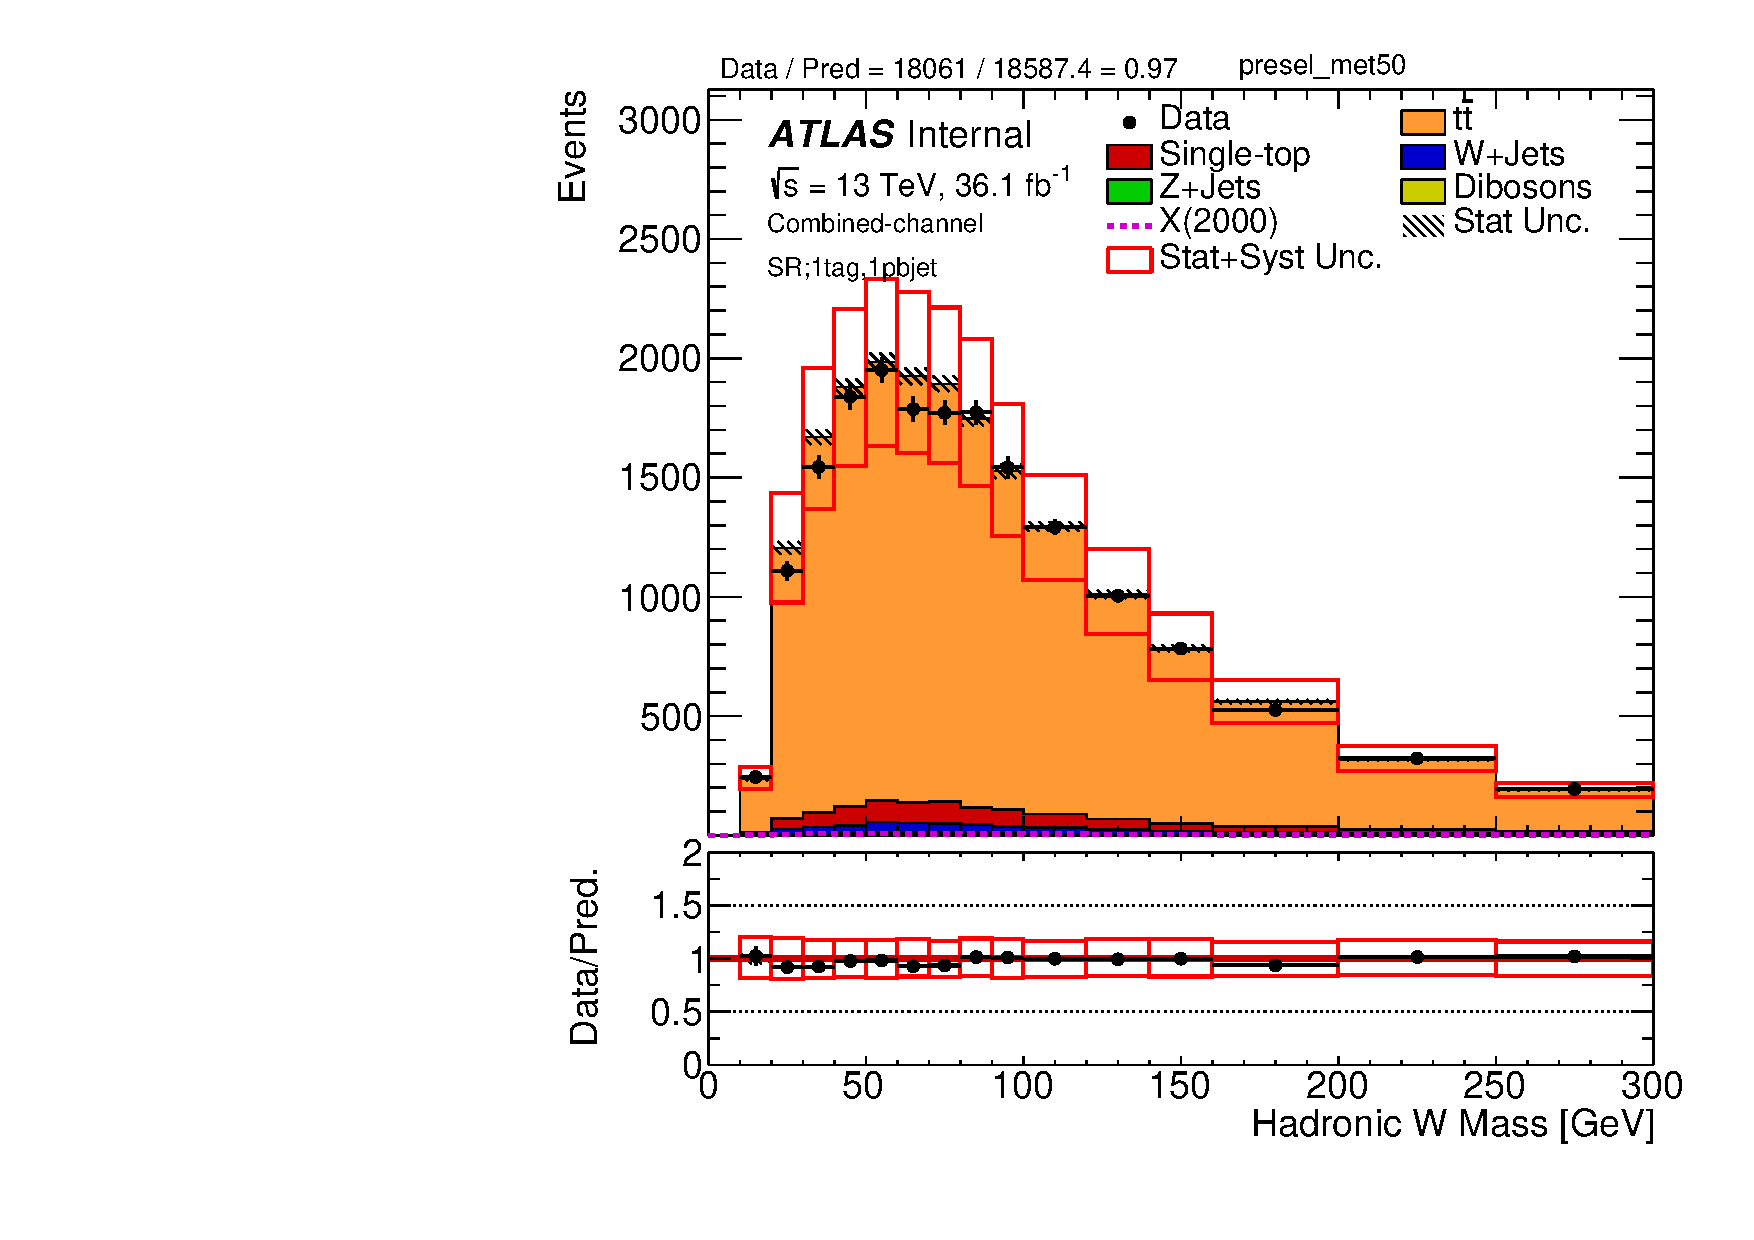
\includegraphics[scale=0.33]{./figures/boosted/Plot1tag1pbjet/DataMC_1tag_1pbjet_SR_lepton_presel_met50_WhadMass}{fig:SR_1tag_1pbjet_whadmass} {Mass} \\
% \par\medskip
% 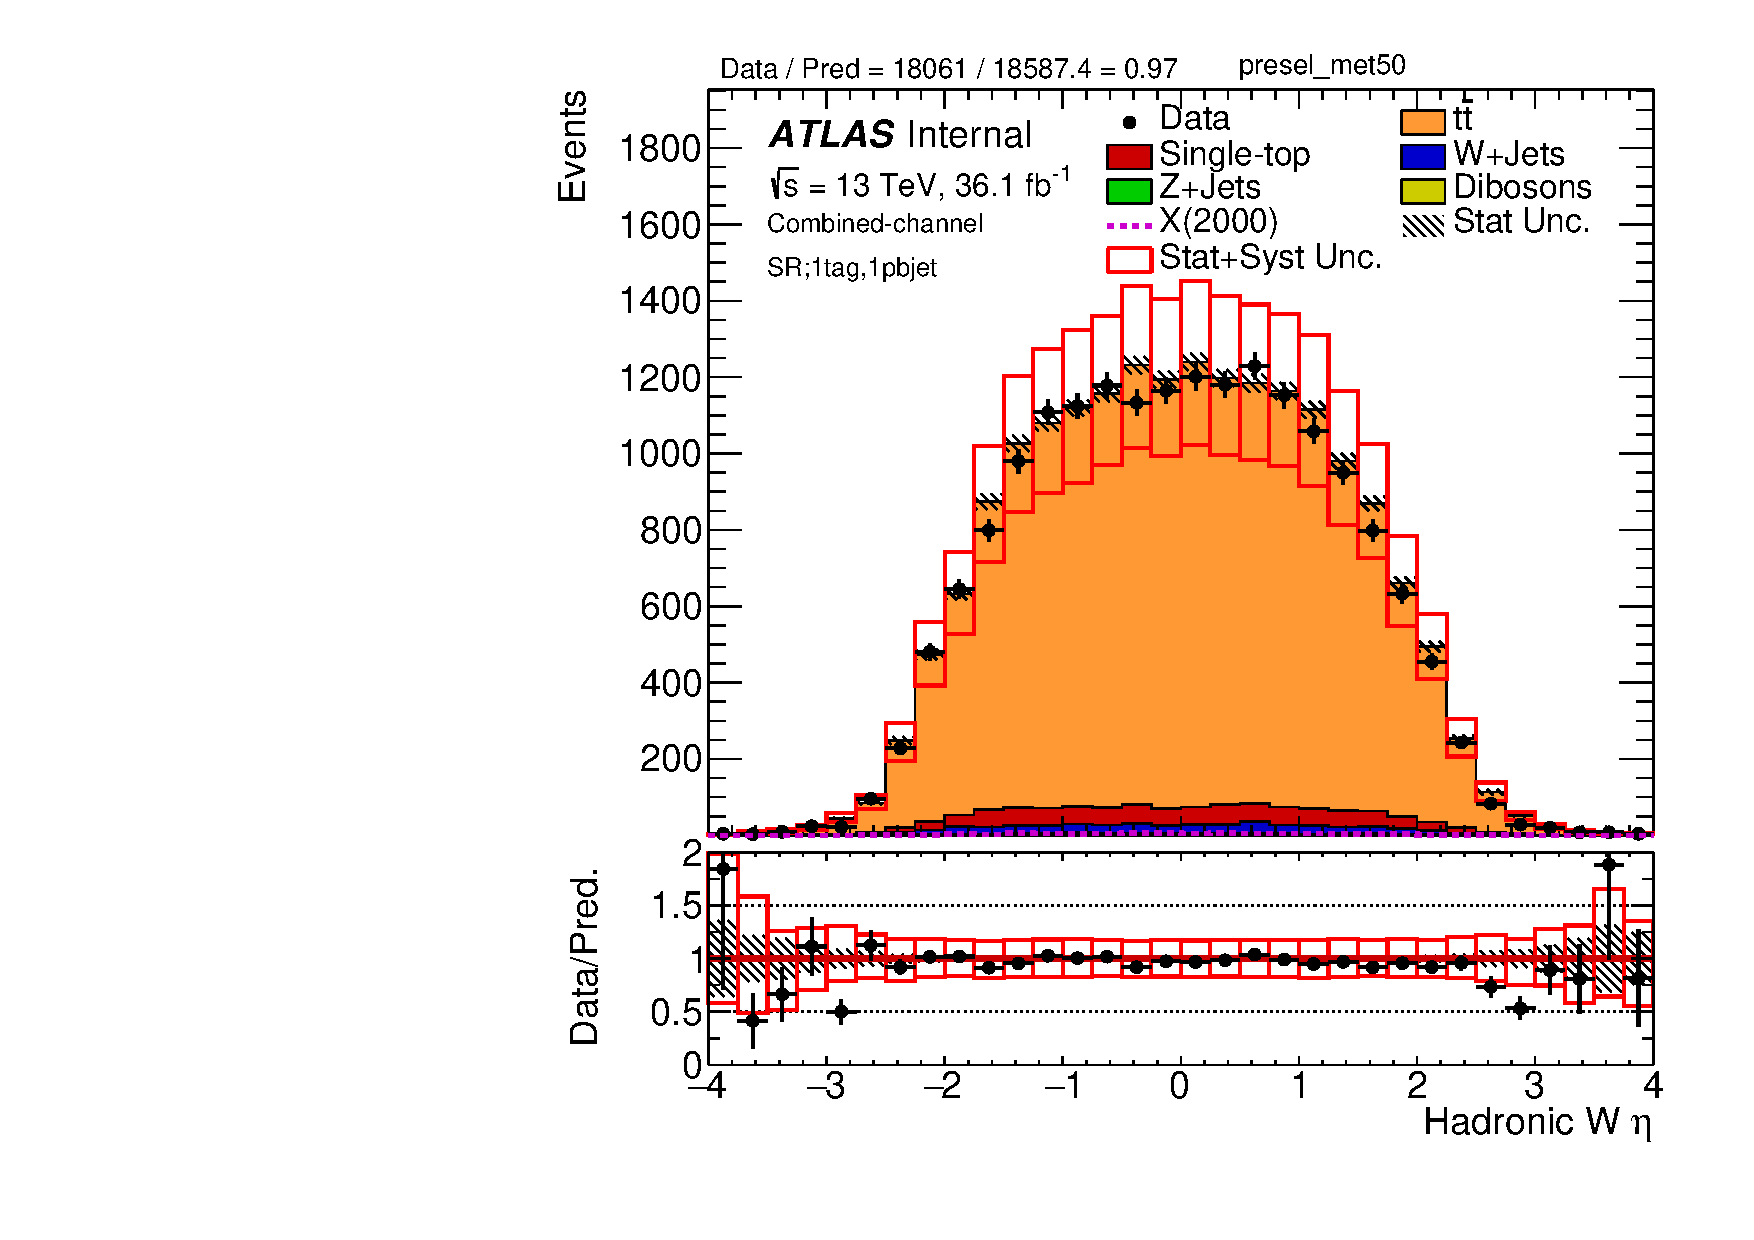
\includegraphics[scale=0.33]{./figures/boosted/Plot1tag1pbjet/DataMC_1tag_1pbjet_SR_lepton_presel_met50_WhadEta}{fig:SR_1tag_1pbjet_whadeta}{$\eta$} 
% 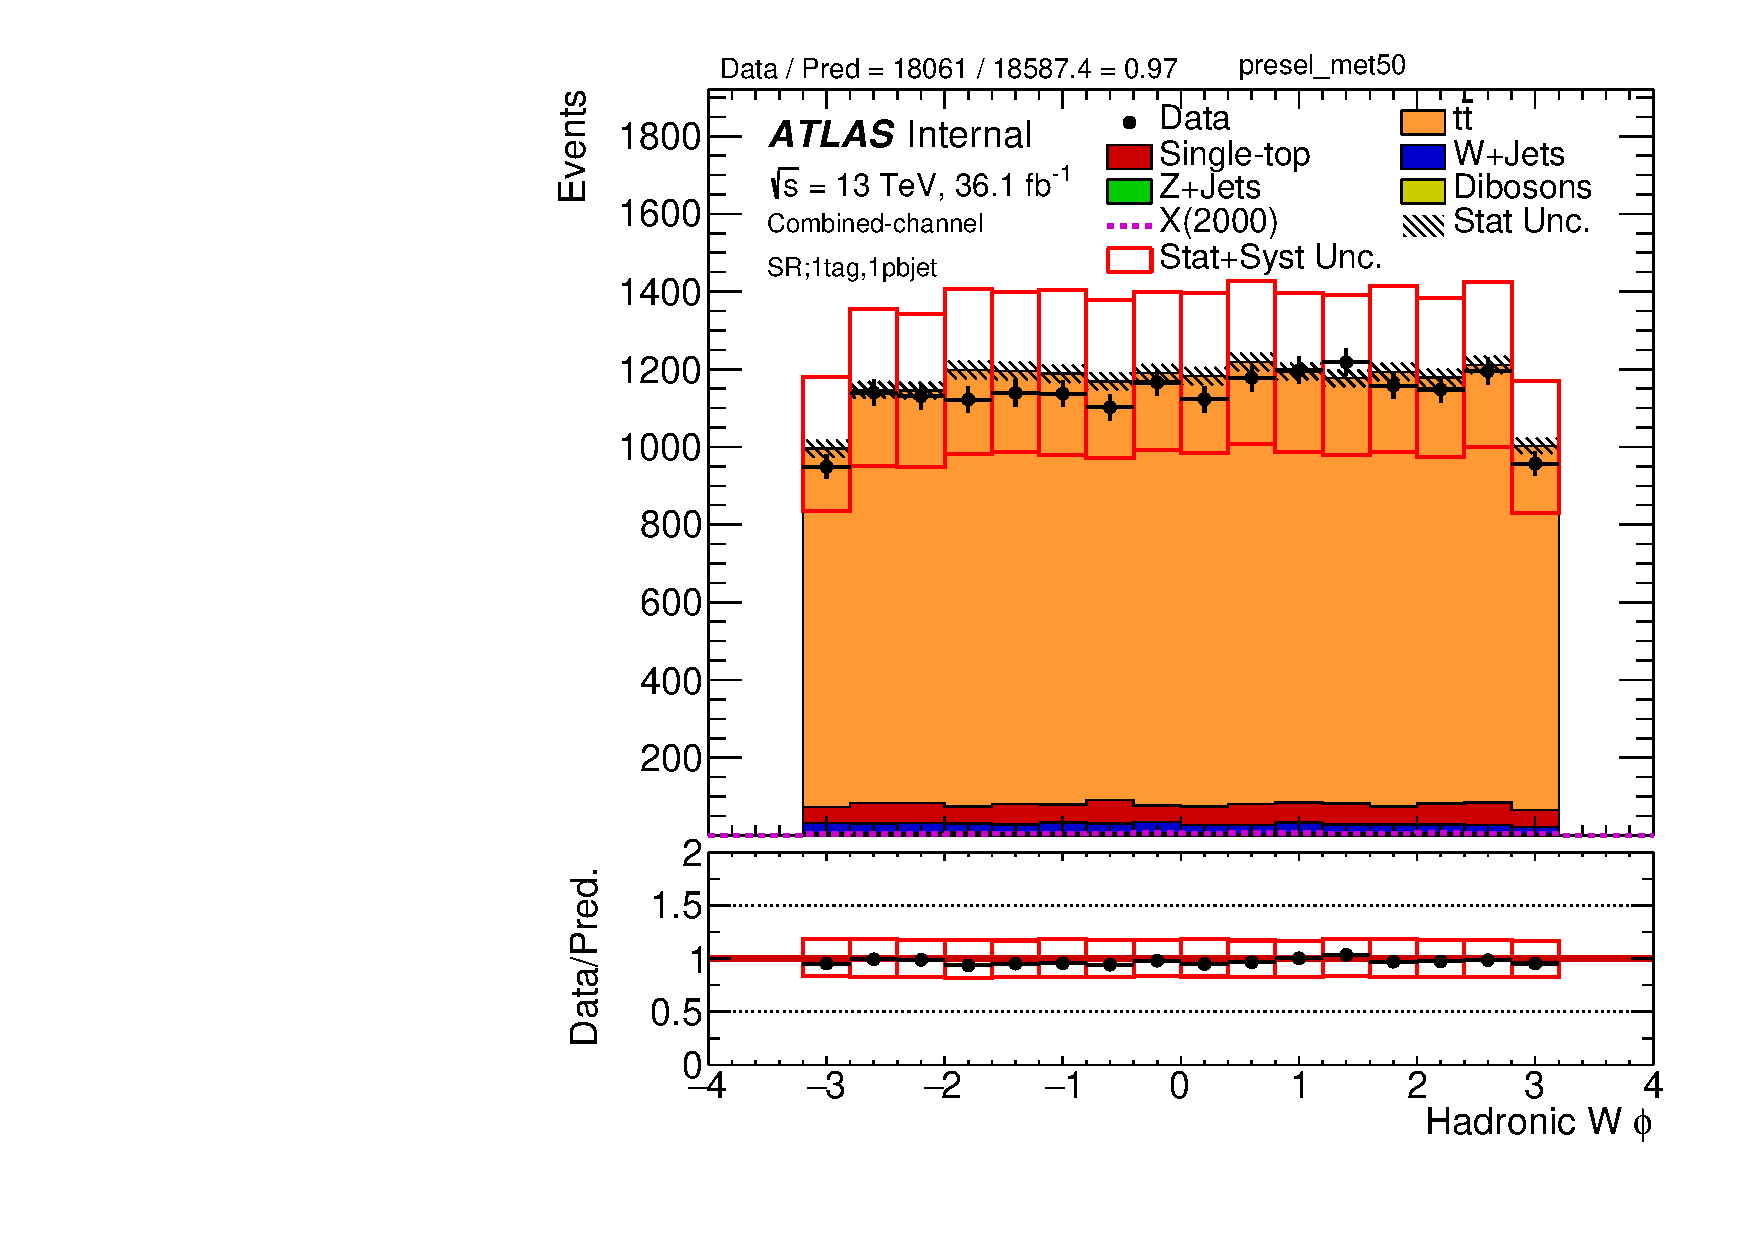
\includegraphics[scale=0.33]{./figures/boosted/Plot1tag1pbjet/DataMC_1tag_1pbjet_SR_lepton_presel_met50_WhadPhi}{fig:SR_1tag_1pbjet_whadphi}{$\phi$}
% \caption{Kinematic distributions of the reconstructed $W \to q\bar{q}$ system in the 1tag,1pbjet signal region.
% All plots are prefit.}
% \label{fig:boosted_SR_1tag_1pbjet_whad}
% \end{center}
% \end{figure}

% \begin{figure}[!h]
% \begin{center}
% 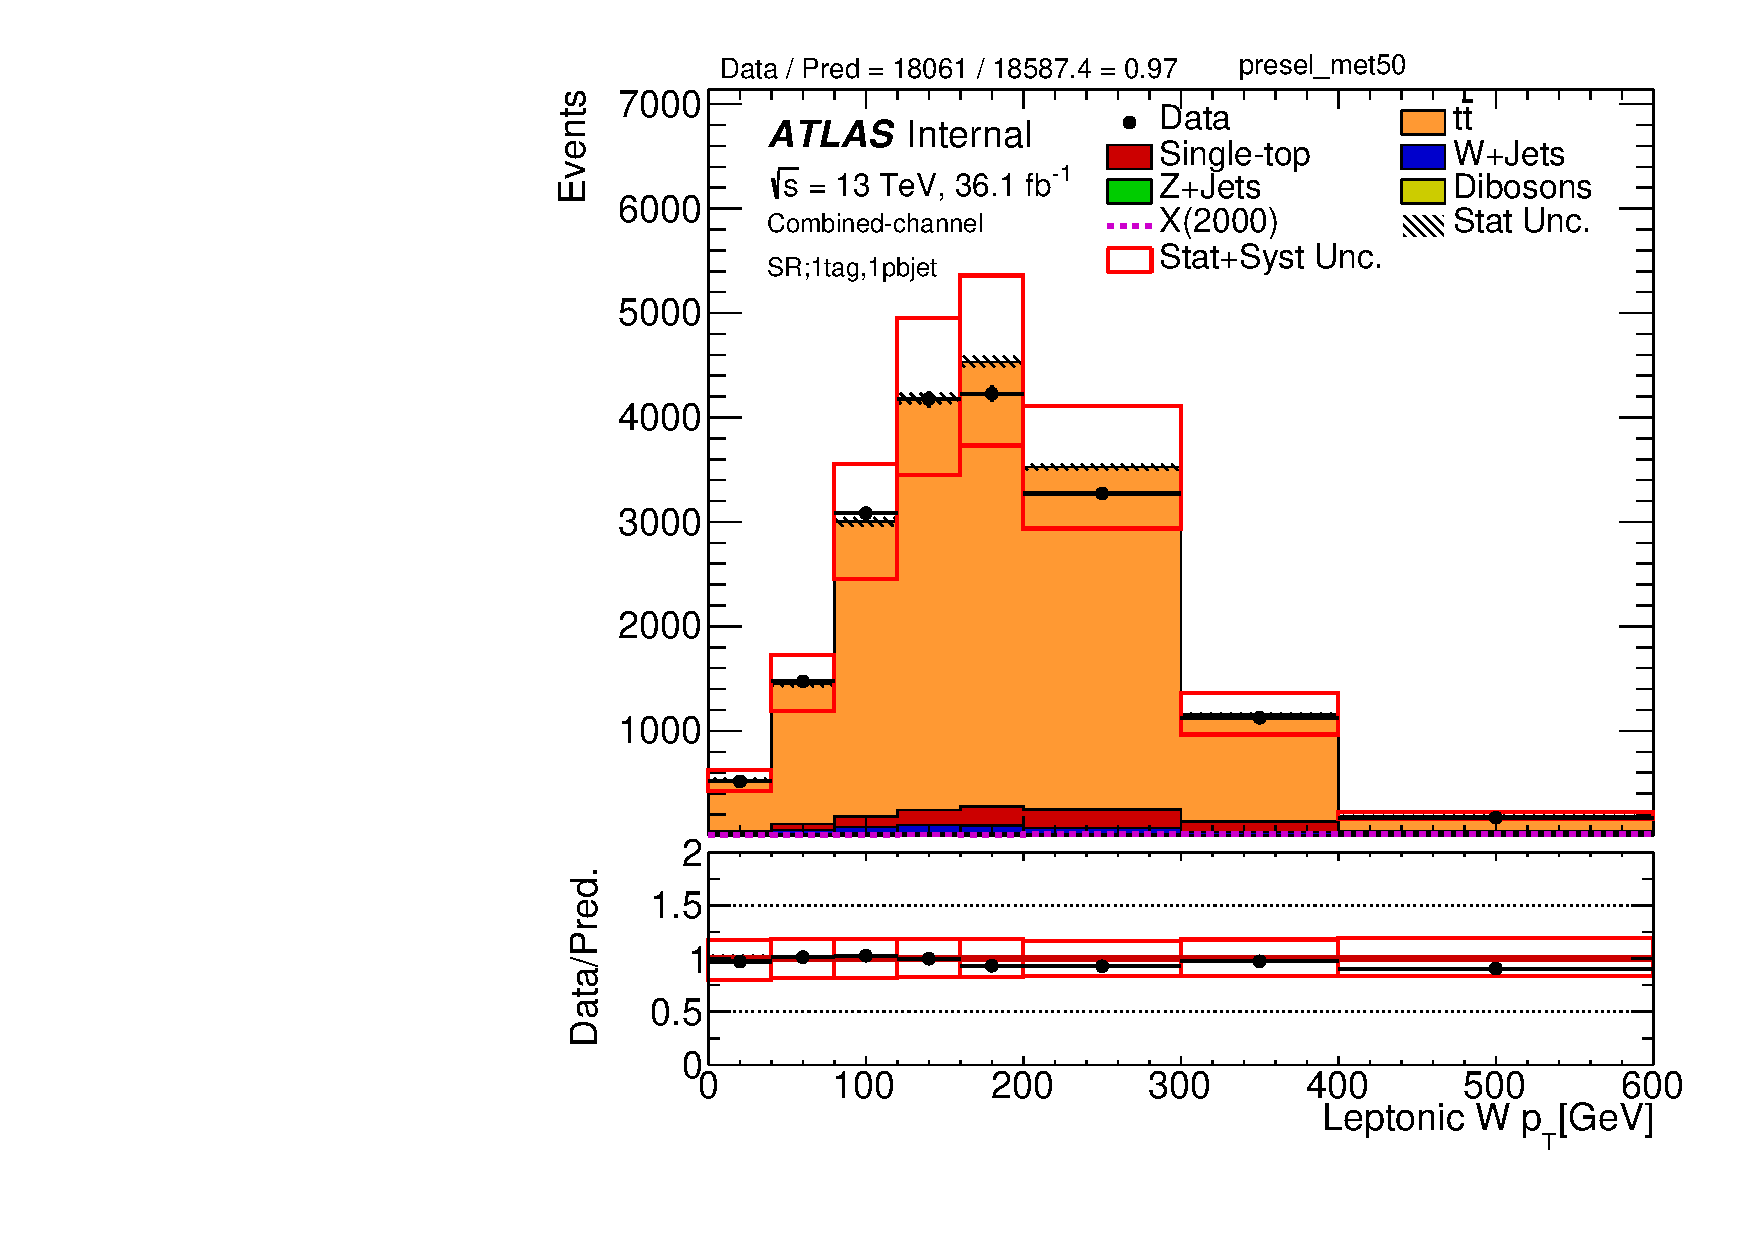
\includegraphics[scale=0.33]{./figures/boosted/Plot1tag1pbjet/DataMC_1tag_1pbjet_SR_lepton_presel_met50_WlepPt}{fig:SR_1tag_1pbjet_wleppt}{\pt} 
% 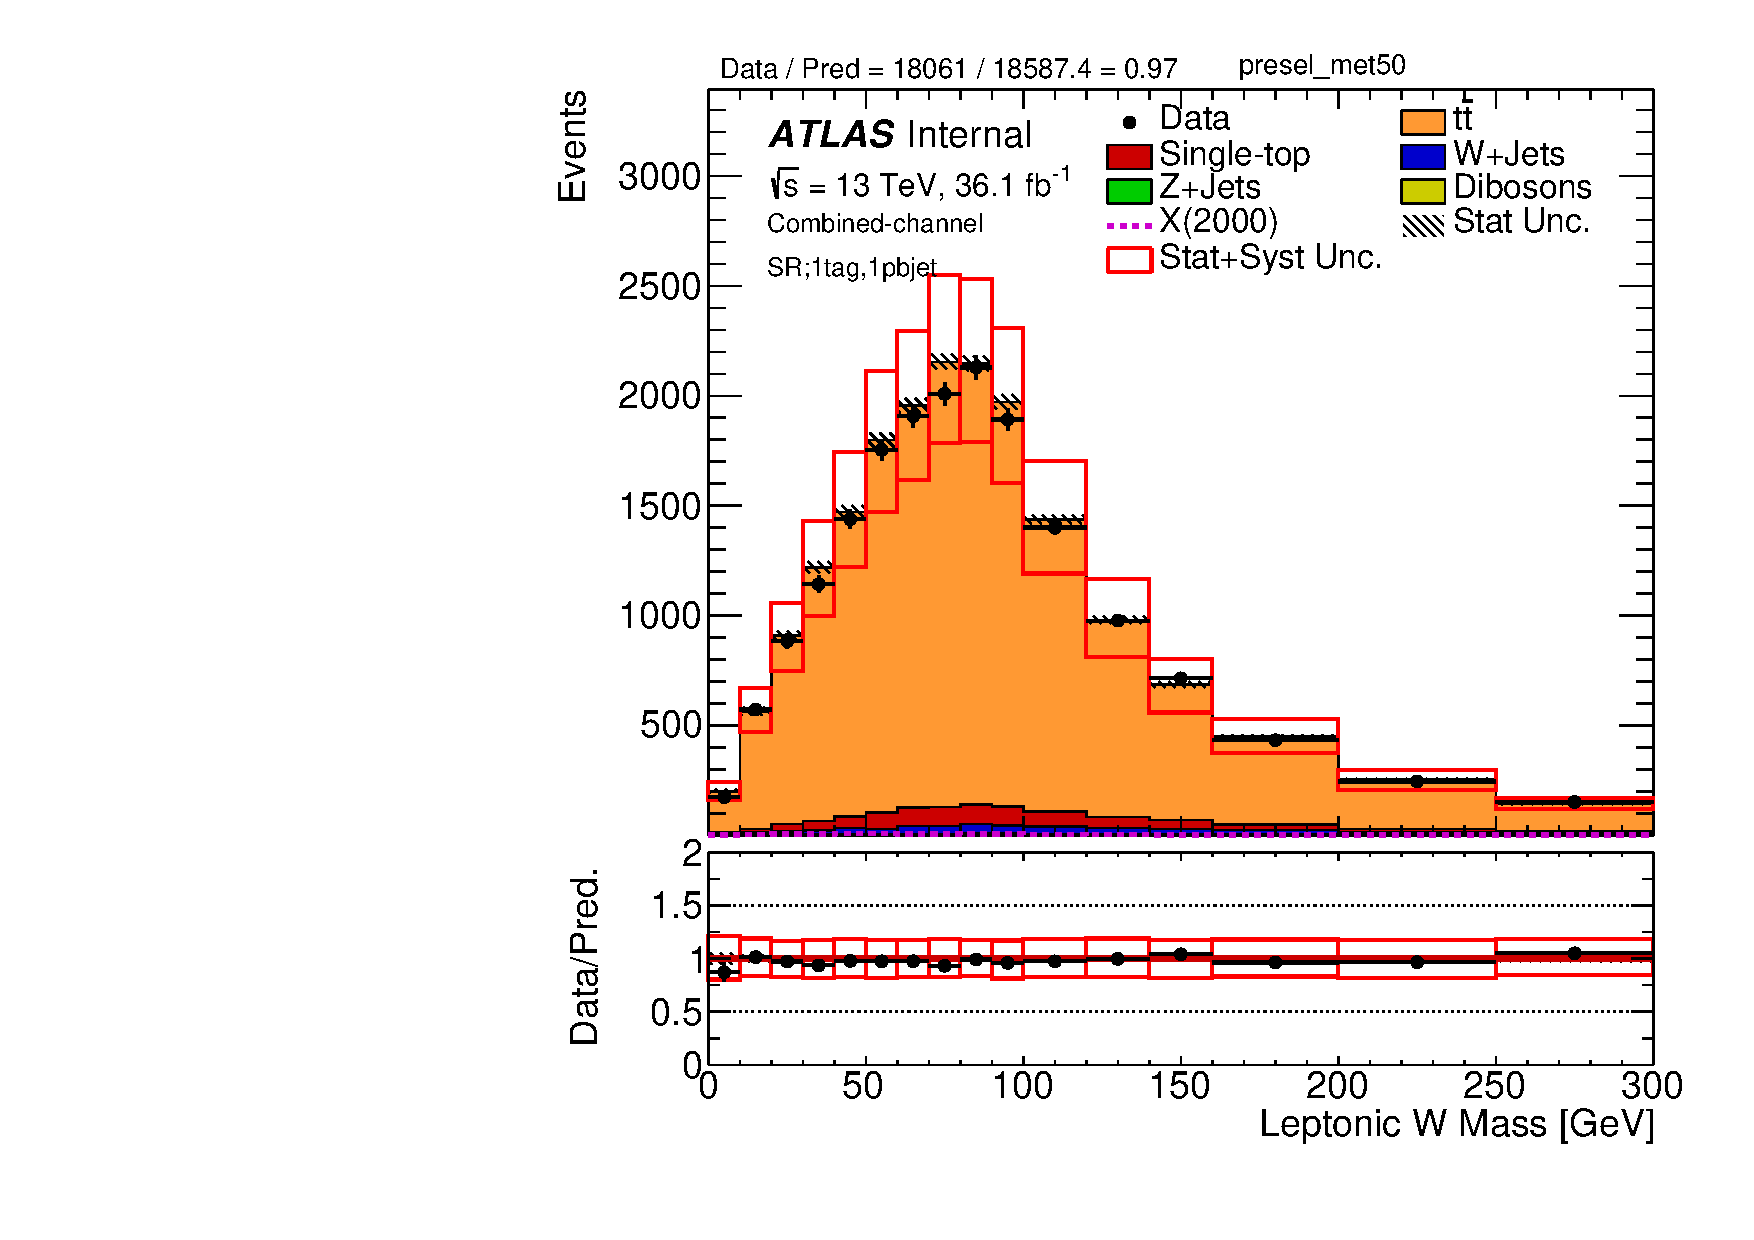
\includegraphics[scale=0.33]{./figures/boosted/Plot1tag1pbjet/DataMC_1tag_1pbjet_SR_lepton_presel_met50_WlepMass}{fig:SR_1tag_1pbjet_wlepmass}{Mass} \\
% \par\medskip
% 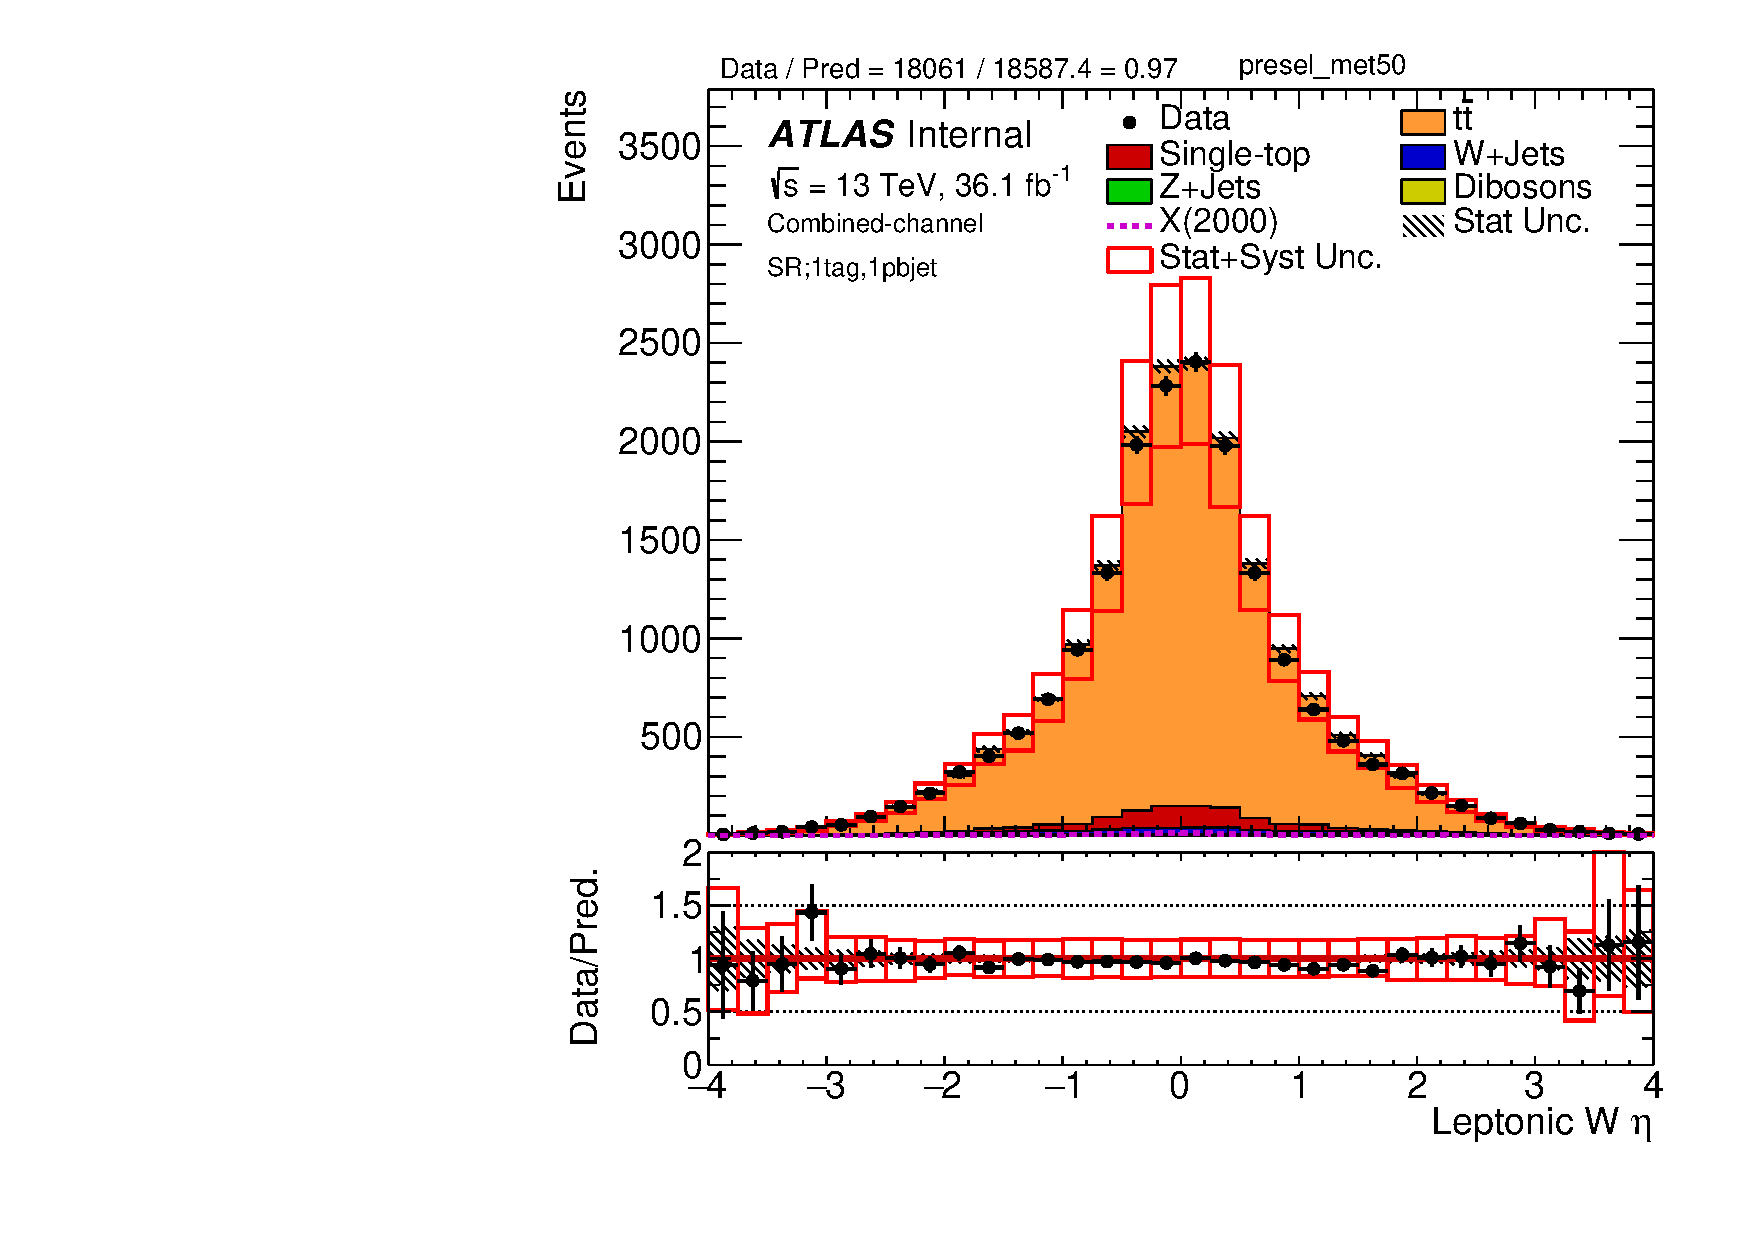
\includegraphics[scale=0.33]{./figures/boosted/Plot1tag1pbjet/DataMC_1tag_1pbjet_SR_lepton_presel_met50_WlepEta}{fig:SR_1tag_1pbjet_wlepeta}{$\eta$} 
% 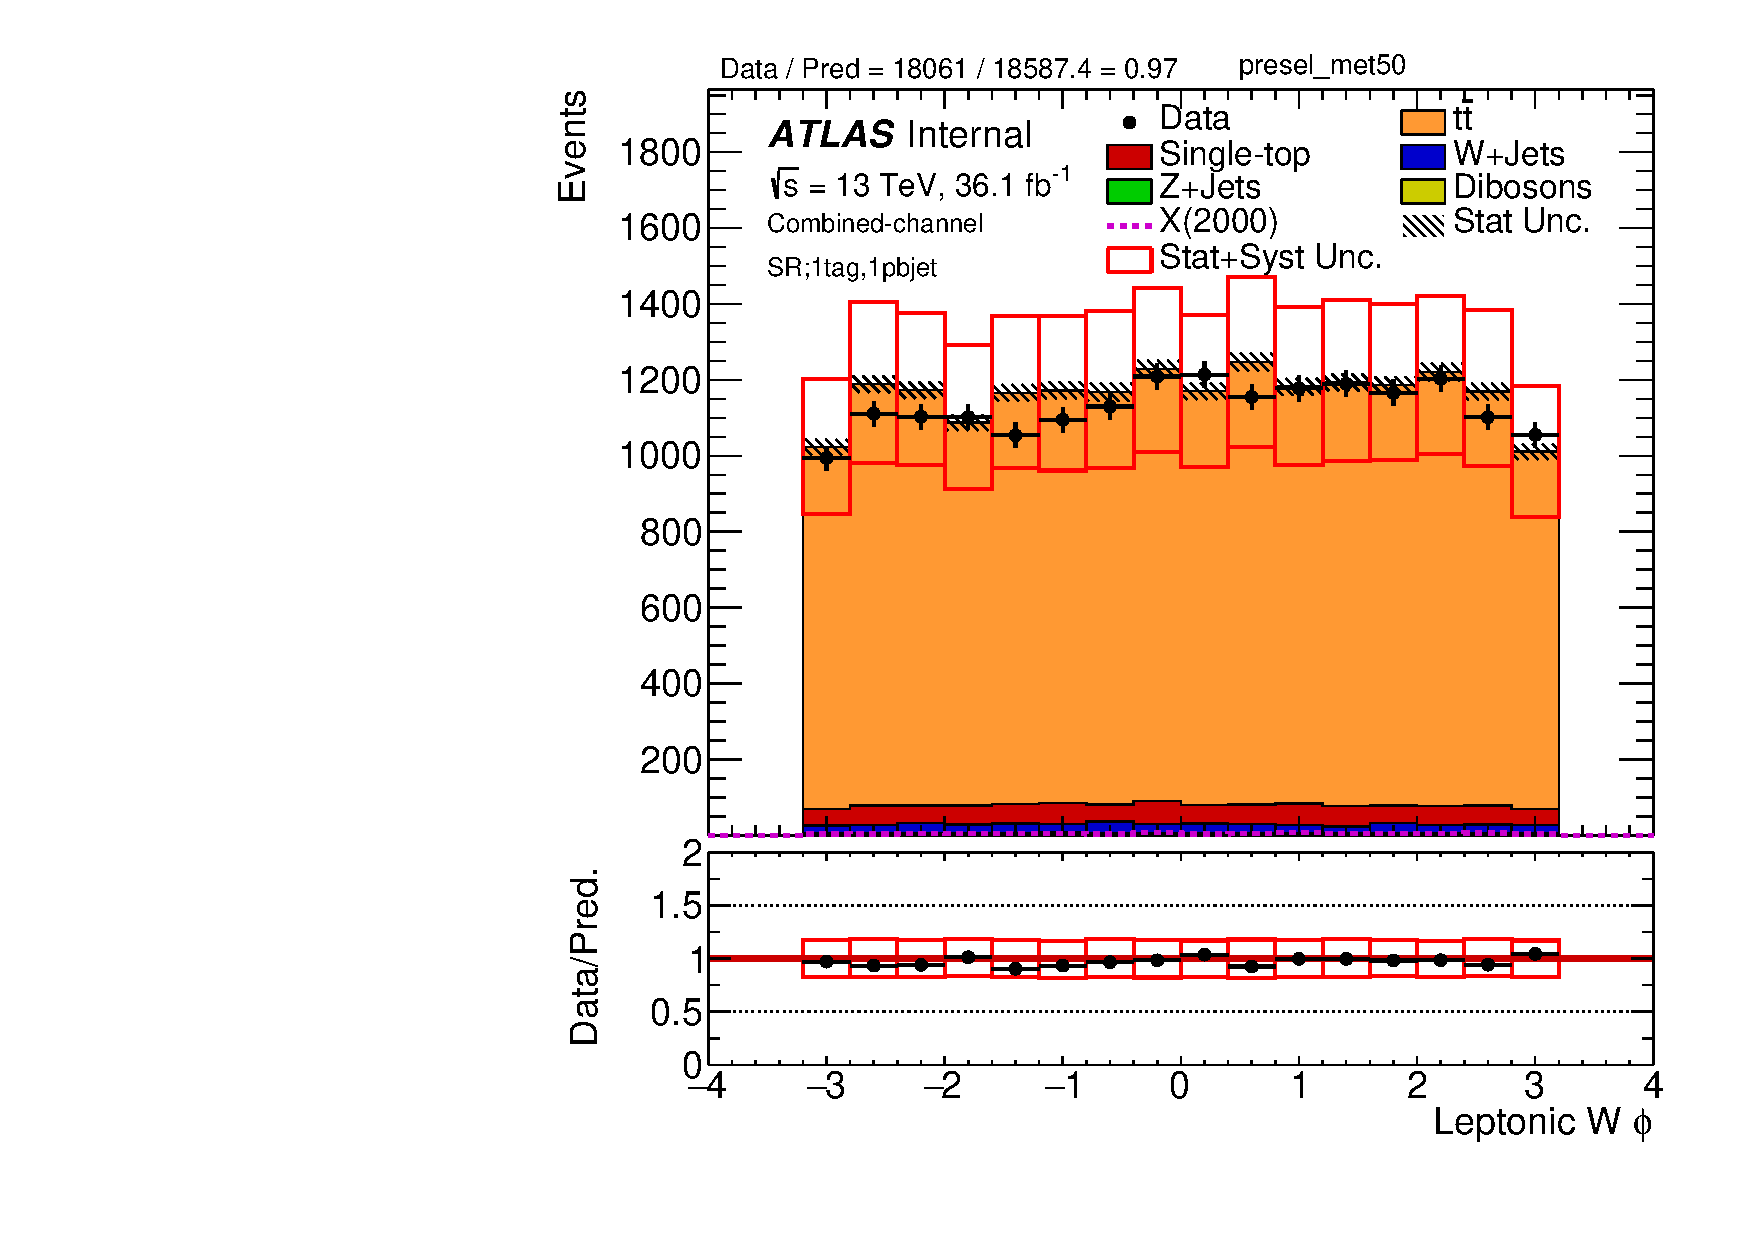
\includegraphics[scale=0.33]{./figures/boosted/Plot1tag1pbjet/DataMC_1tag_1pbjet_SR_lepton_presel_met50_WlepPhi}{fig:SR_1tag_1pbjet_wlepphi}{$\phi$}
% \caption{Kinematic distributions of the reconstructed $W \to l\nu$ system in the 1tag,1pbjet signal region.
% All plots are prefit.}
% \label{fig:boosted_SR_1tag_1pbjet_wlep}
% \end{center}
% \end{figure}

\begin{figure}[!h]
\begin{center}
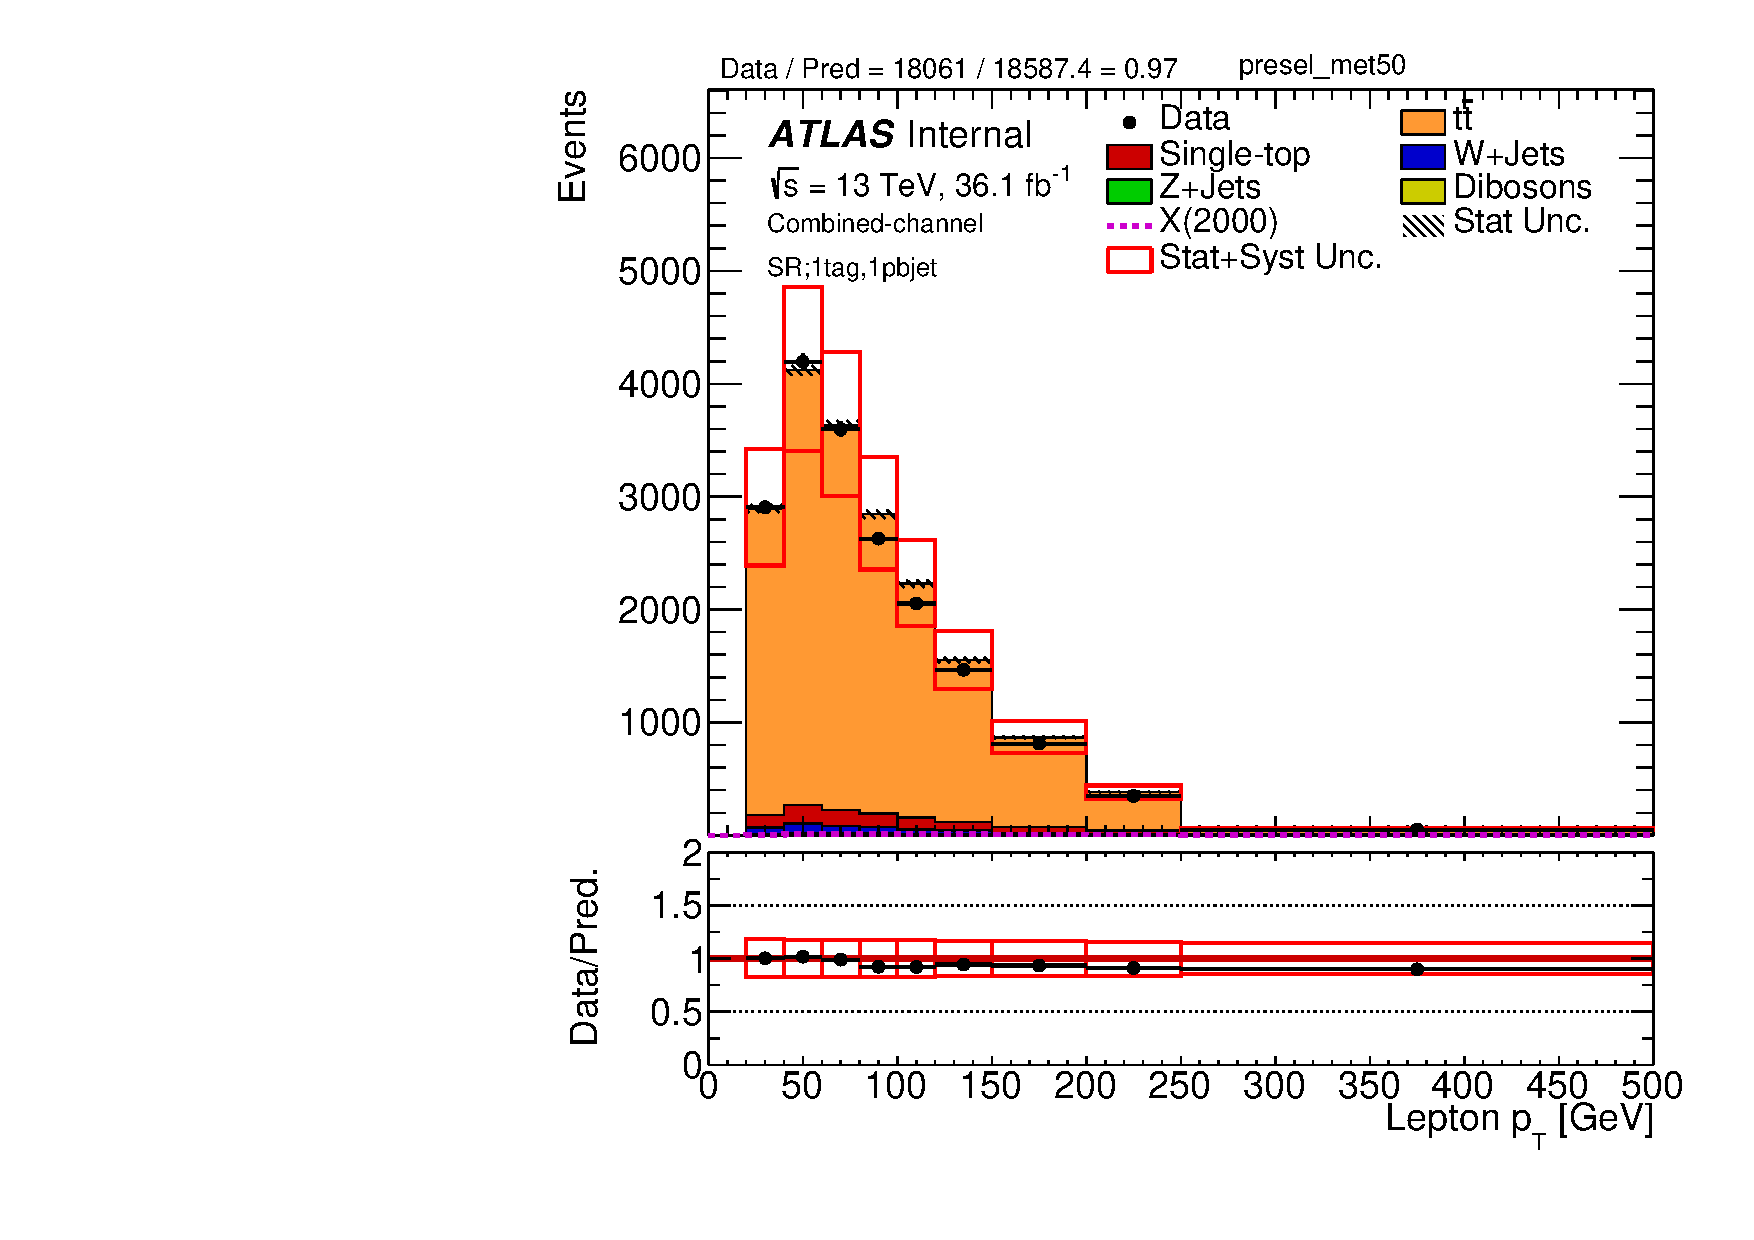
\includegraphics[scale=0.33]{./figures/boosted/Plot1tag1pbjet/DataMC_1tag_1pbjet_SR_lepton_presel_met50_LepPt}\\
\par\medskip
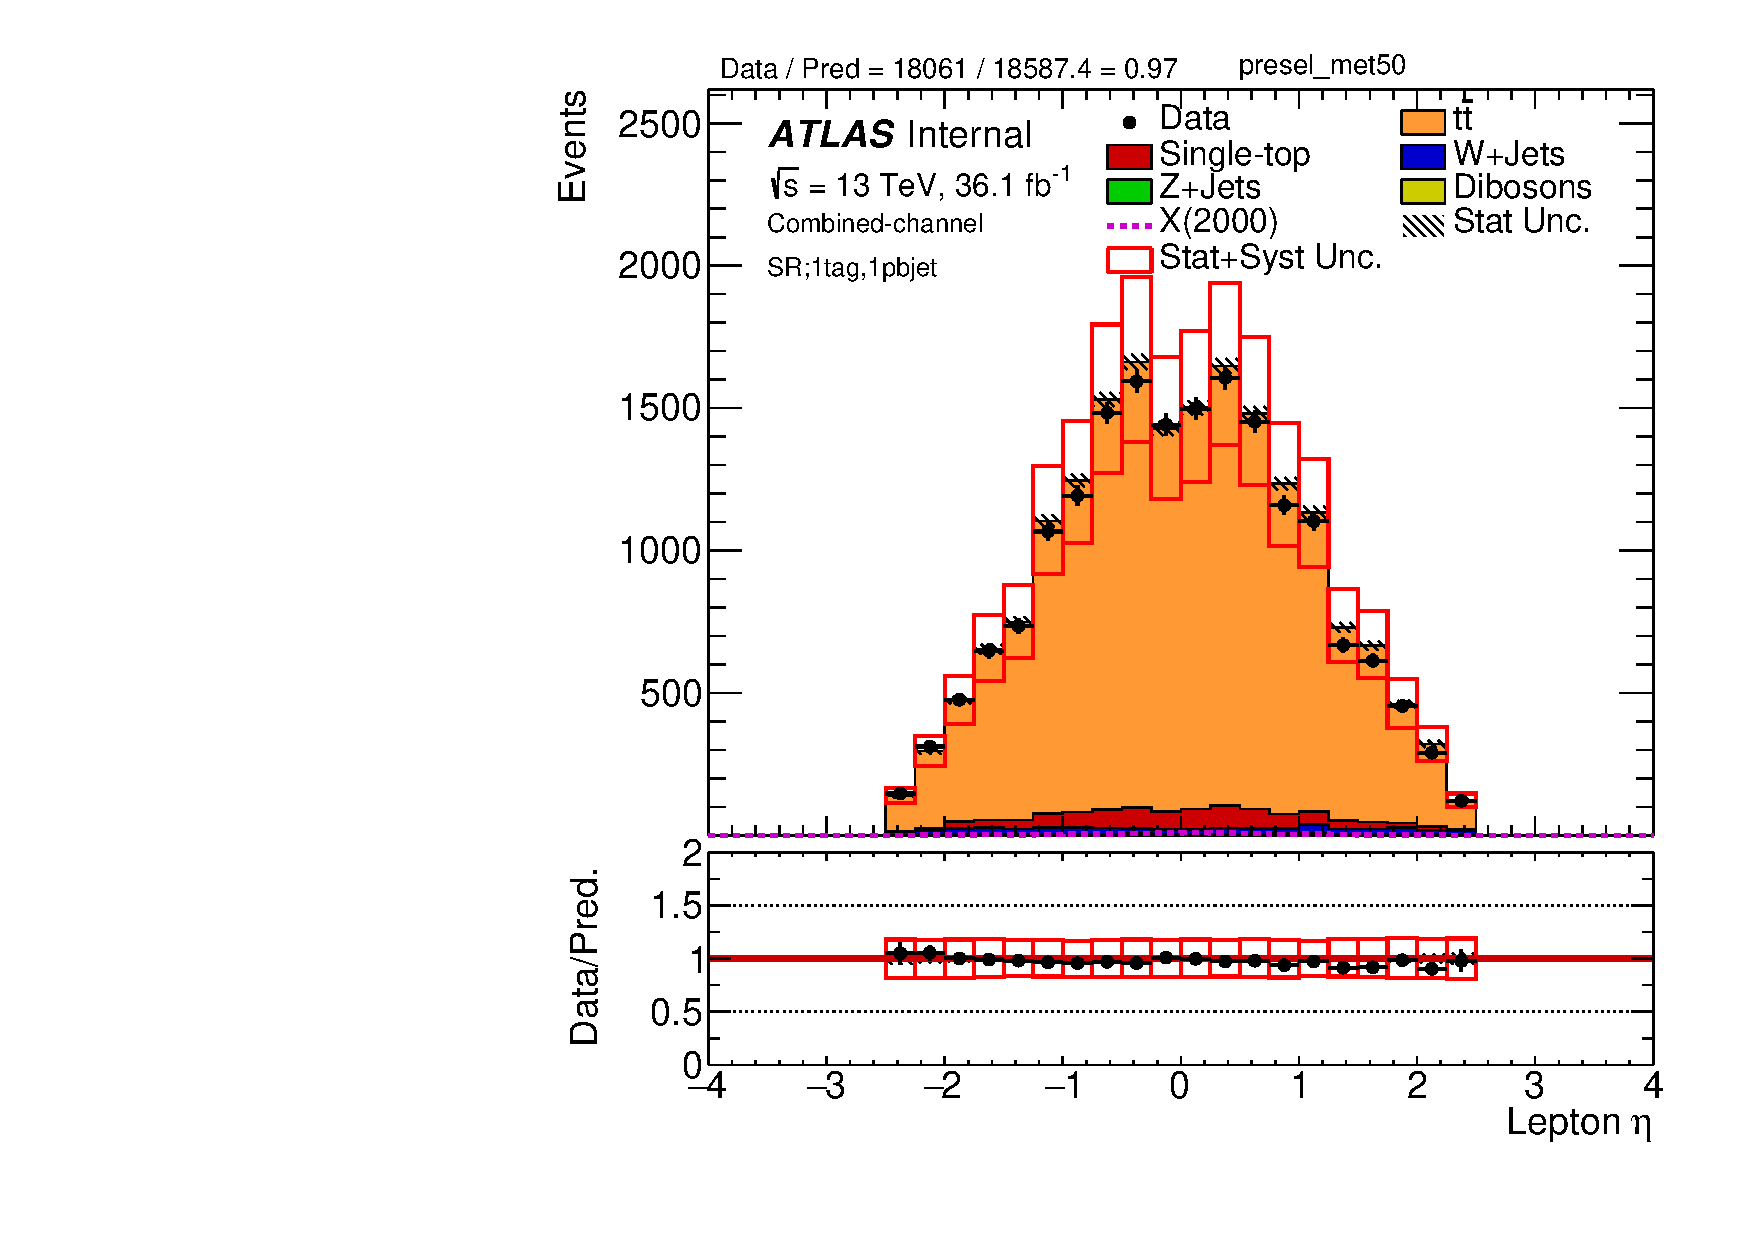
\includegraphics[scale=0.33]{./figures/boosted/Plot1tag1pbjet/DataMC_1tag_1pbjet_SR_lepton_presel_met50_LepEta}
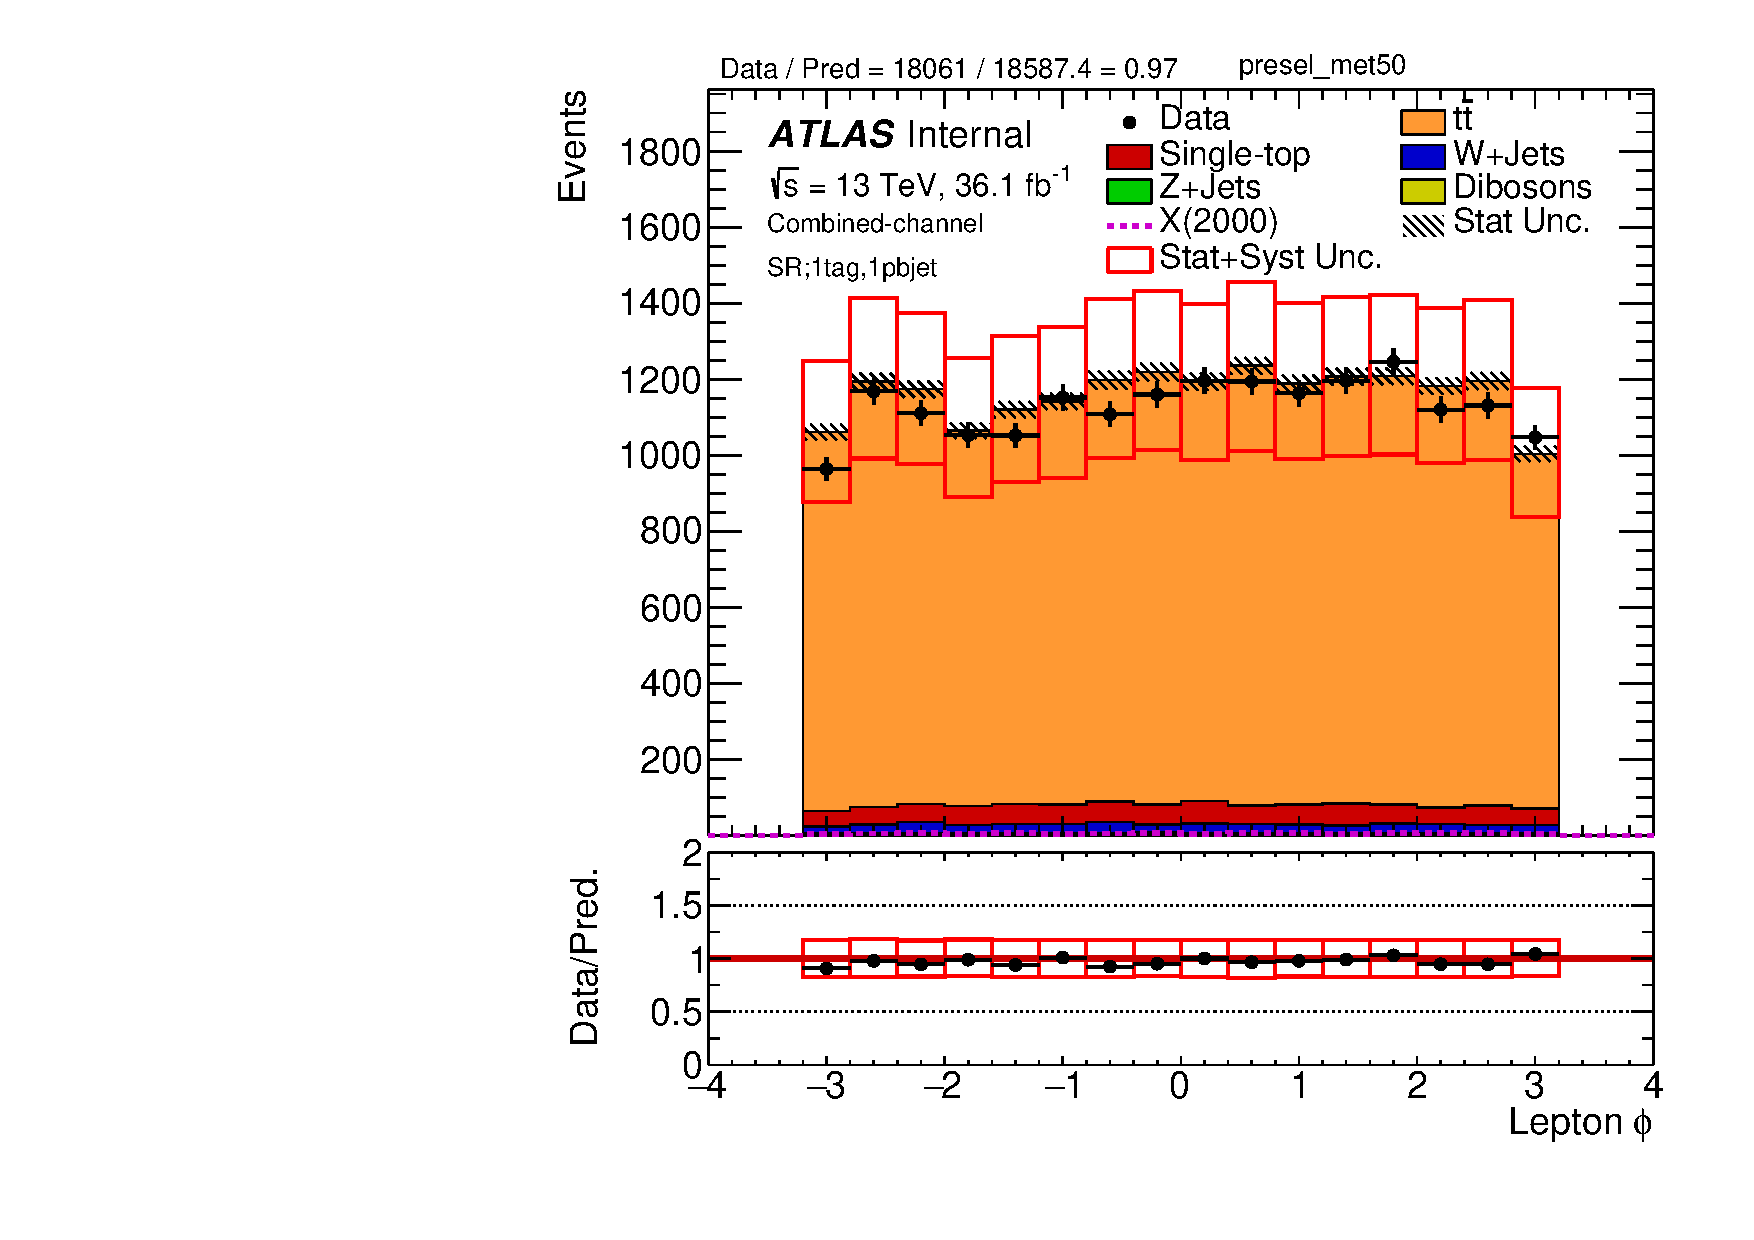
\includegraphics[scale=0.33]{./figures/boosted/Plot1tag1pbjet/DataMC_1tag_1pbjet_SR_lepton_presel_met50_LepPhi} 
\caption{Kinematic distributions of the selected lepton in the 1tag,1pbjet signal region. All plots are prefit.}
\label{fig:boosted_SR_1tag_1pbjet_lepton}
\end{center}
\end{figure}


% \begin{figure}[!ht]
% \begin{center}
% 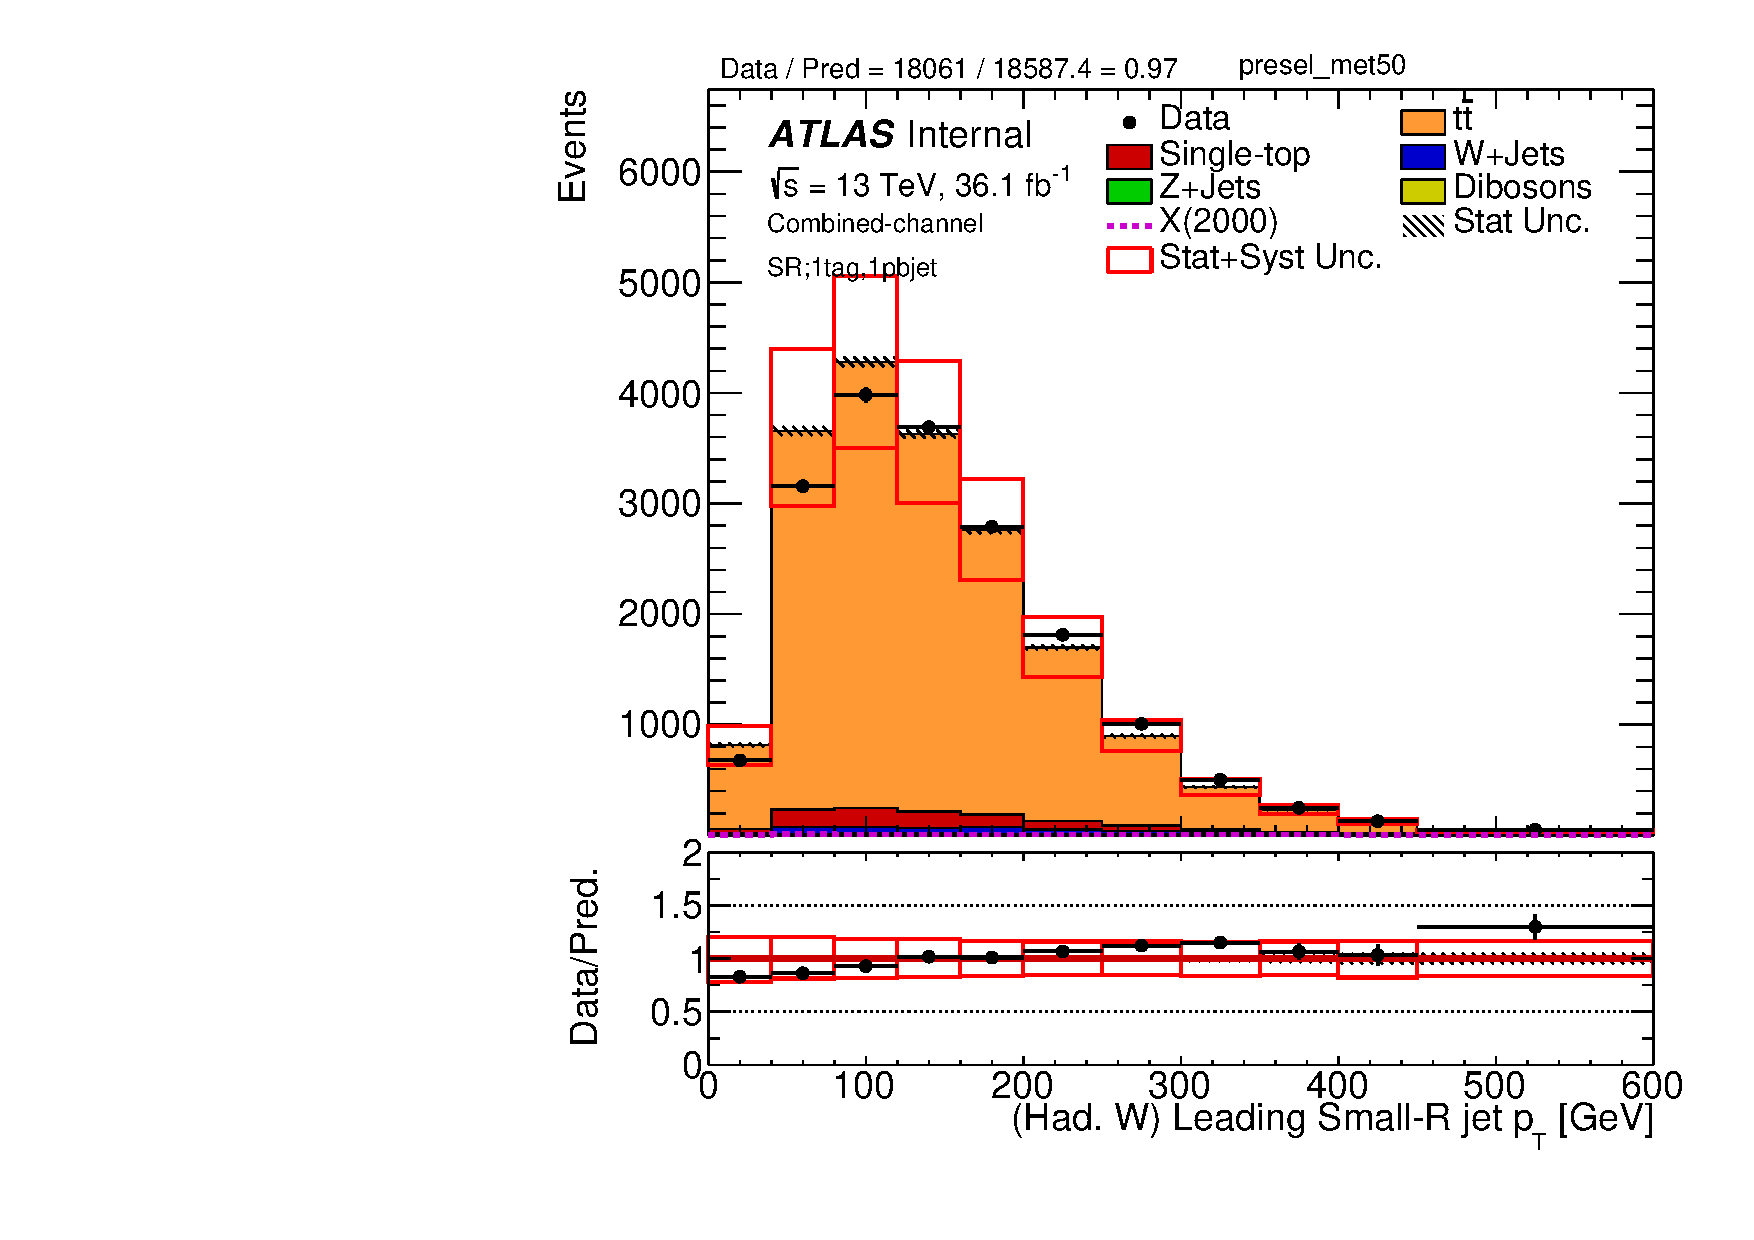
\includegraphics[scale=0.33]{./figures/boosted/Plot1tag1pbjet/DataMC_1tag_1pbjet_SR_lepton_presel_met50_LightJet1Pt}{fig:SR_1tag_1pbjet_jet1_pt}{Leading jet \pt}
% 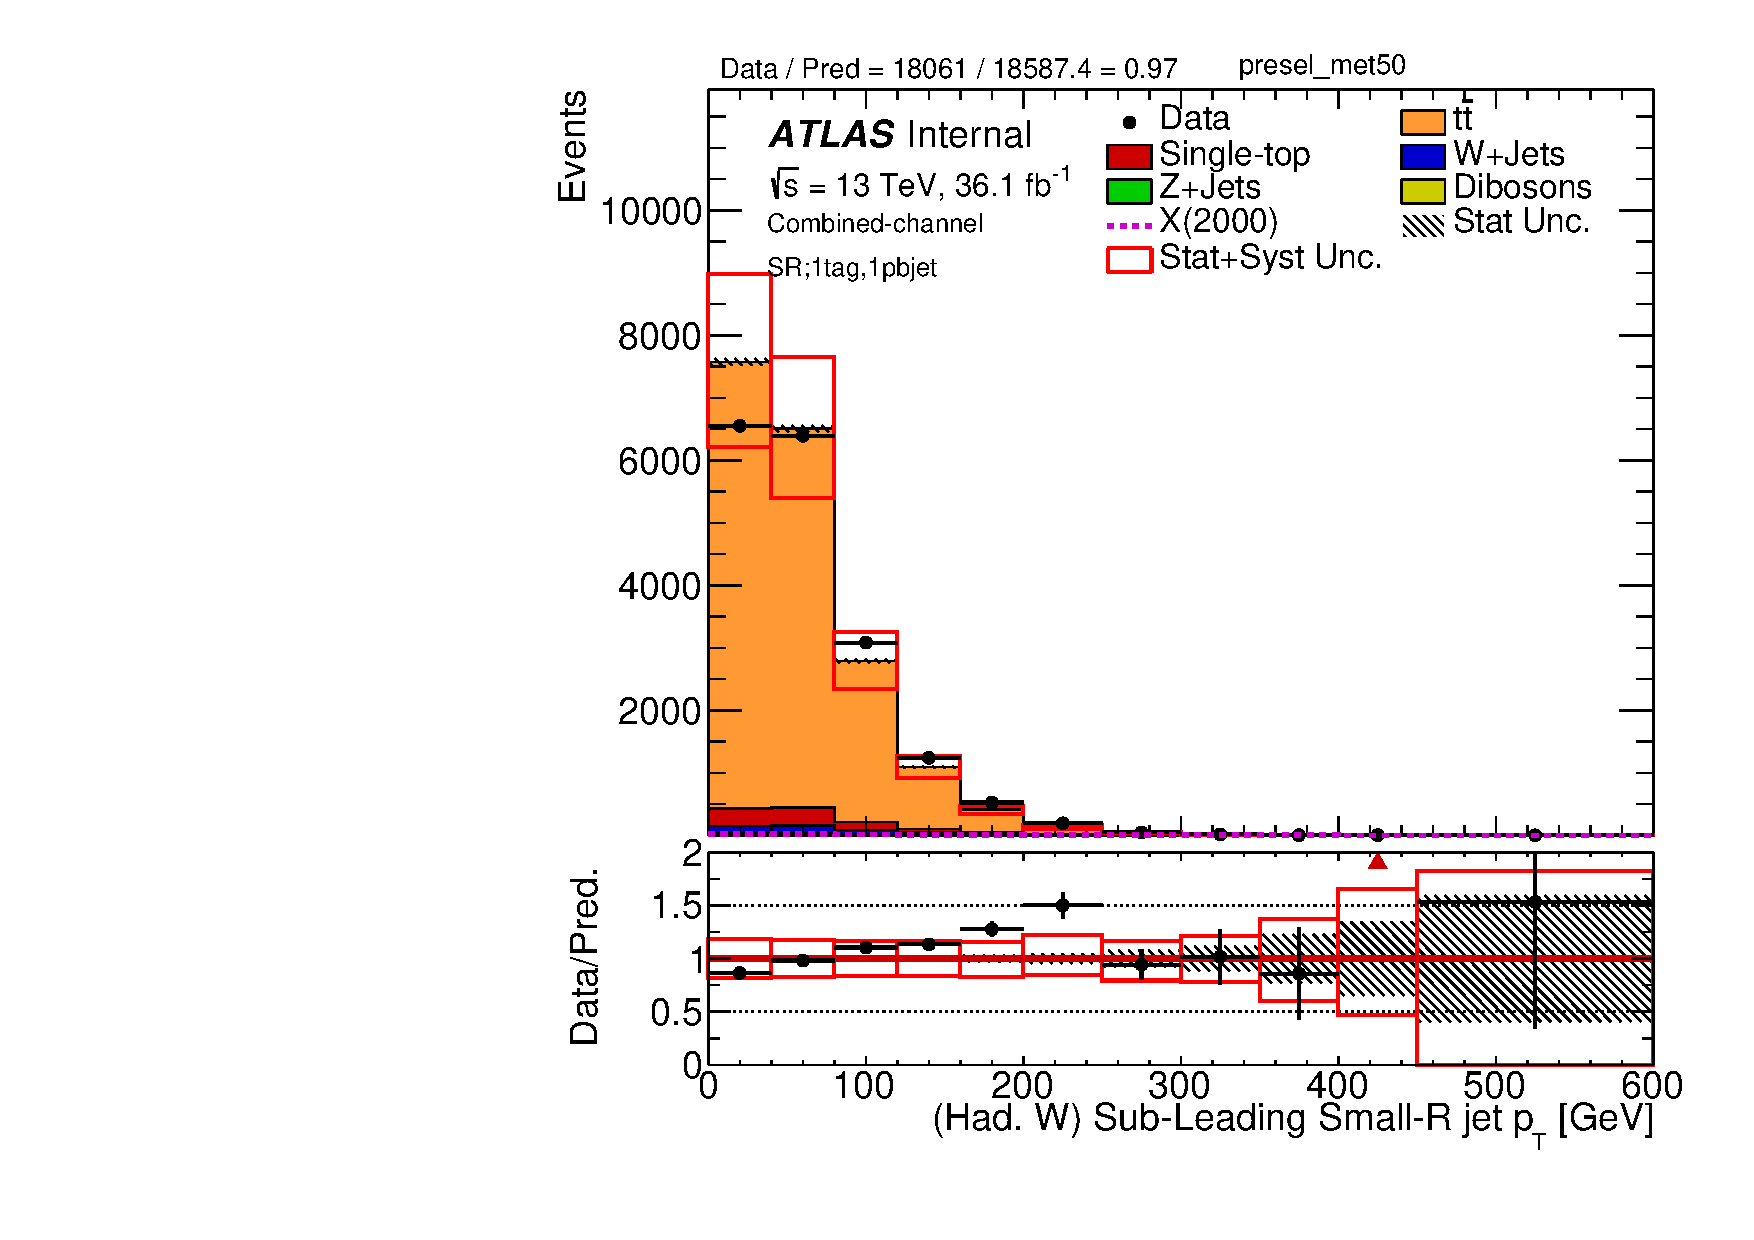
\includegraphics[scale=0.33]{./figures/boosted/Plot1tag1pbjet/DataMC_1tag_1pbjet_SR_lepton_presel_met50_LightJet2Pt}{fig:SR_1tag_1pbjet_jet2_pt}{Sub-leading jet \pt}\\
% \par\medskip
% 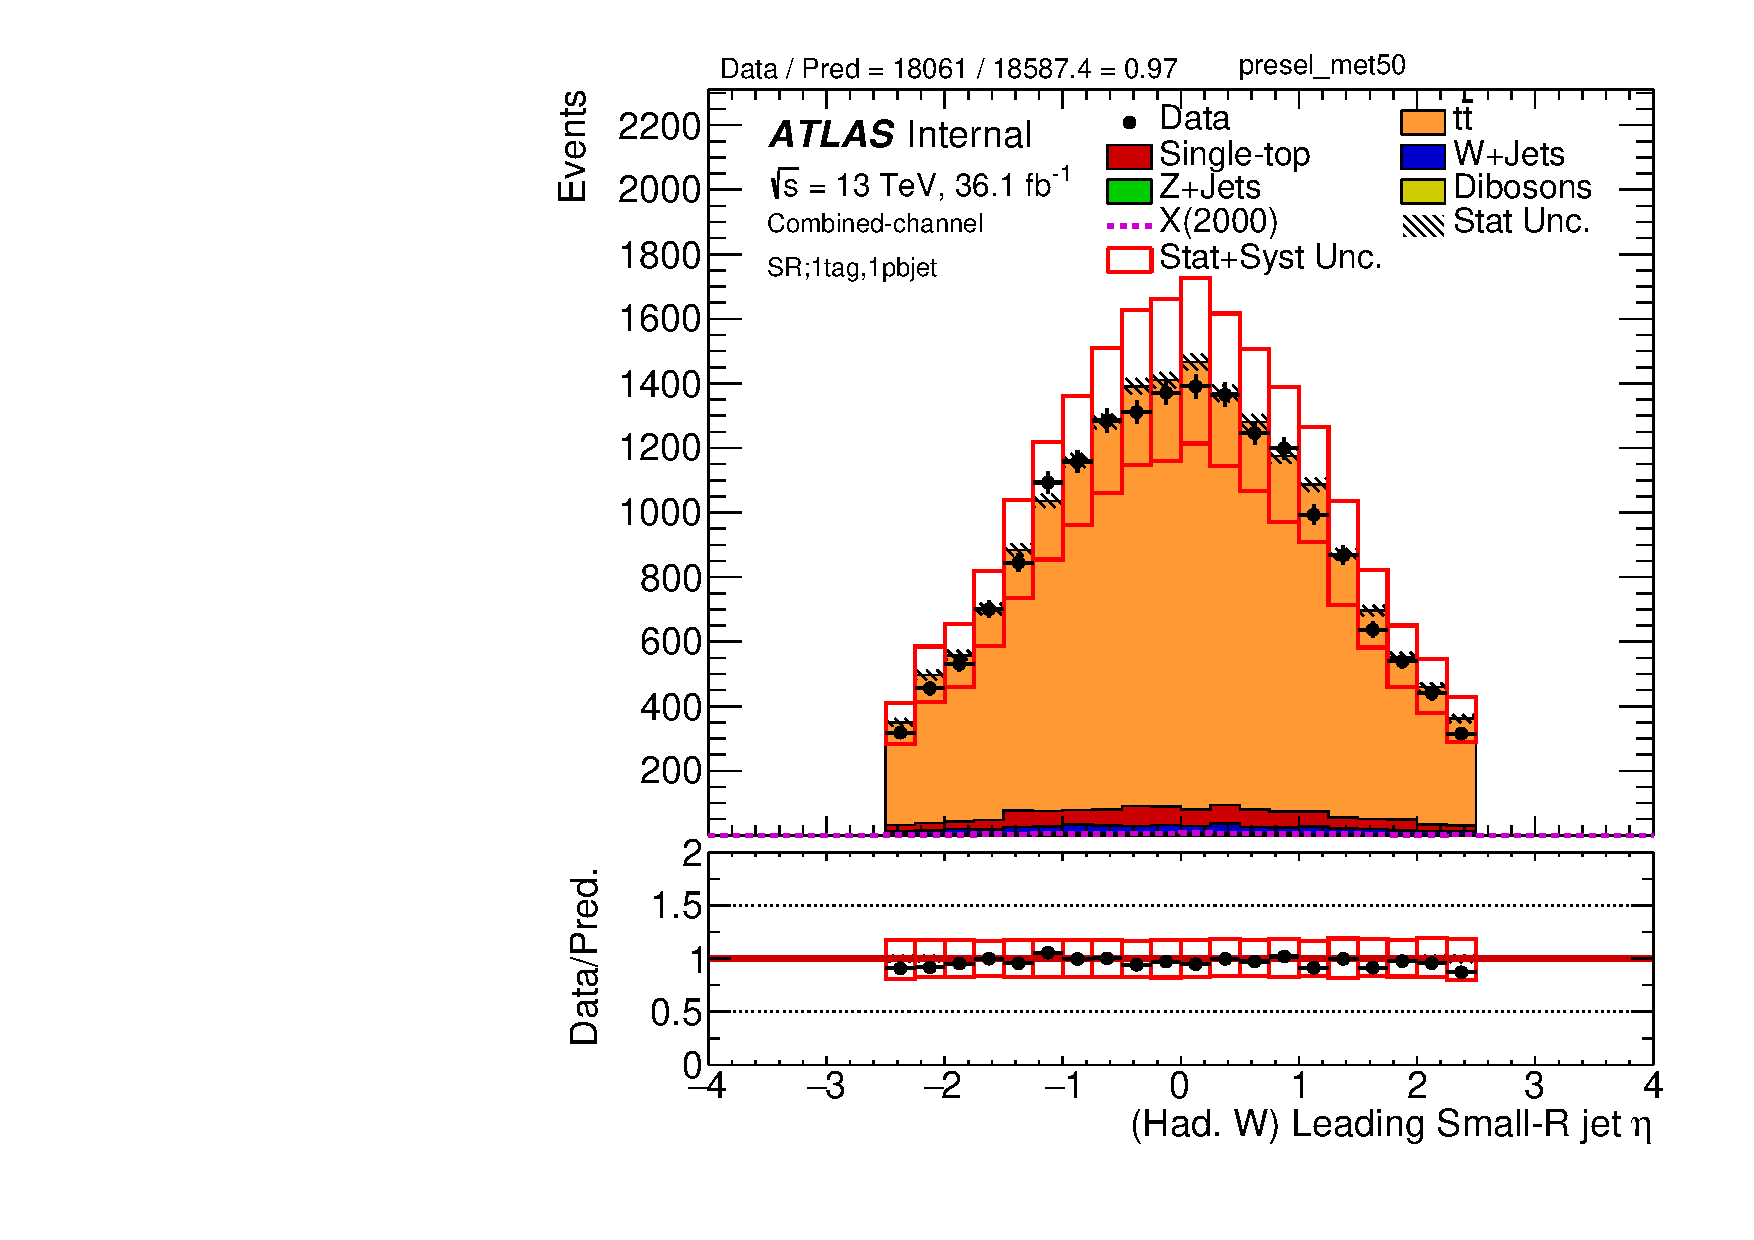
\includegraphics[scale=0.33]{./figures/boosted/Plot1tag1pbjet/DataMC_1tag_1pbjet_SR_lepton_presel_met50_LightJet1Eta}{fig:SR_1tag_1pbjet_jet1_eta}{Leading jet $\eta$}
% 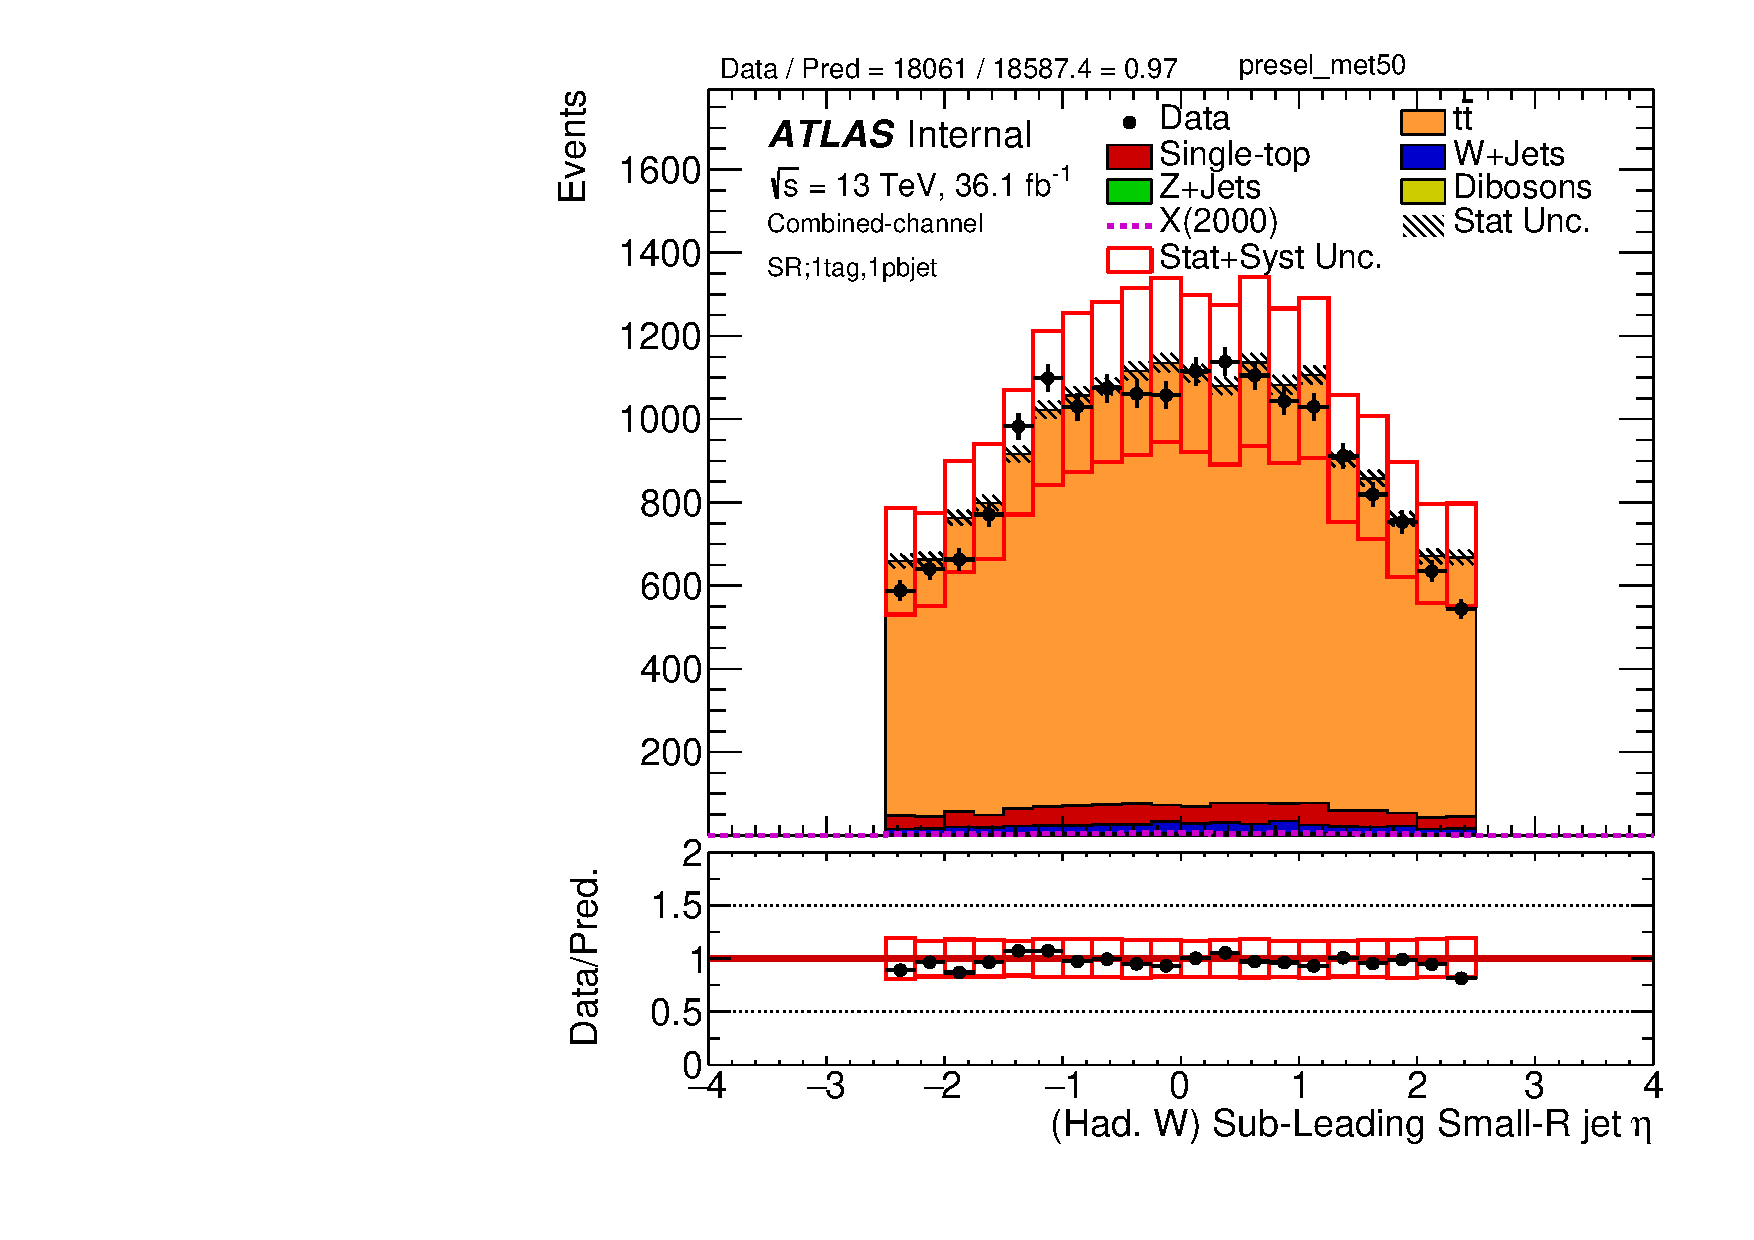
\includegraphics[scale=0.33]{./figures/boosted/Plot1tag1pbjet/DataMC_1tag_1pbjet_SR_lepton_presel_met50_LightJet2Eta}{fig:SR_1tag_1pbjet_jet2_eta}{Sub-leading jet $\eta$}\\
% \par\medskip
% 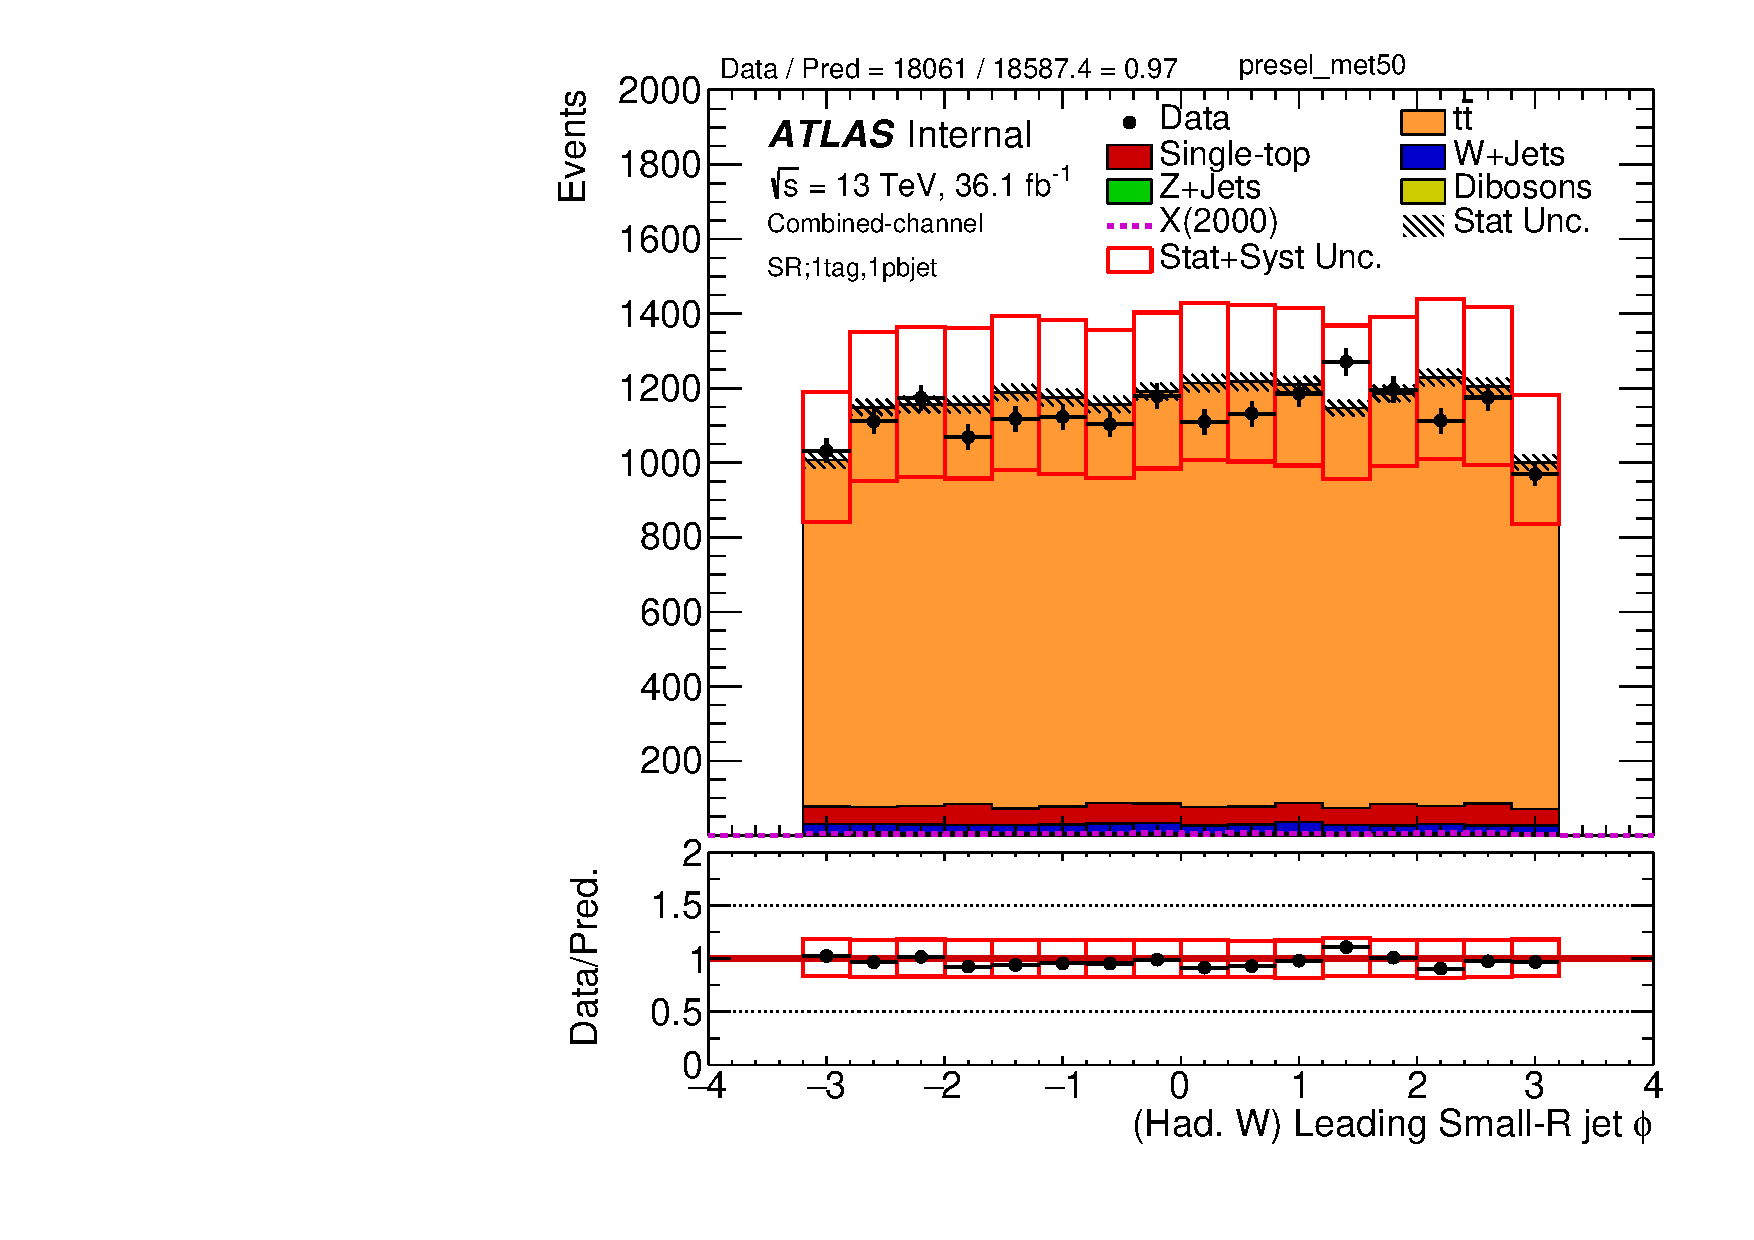
\includegraphics[scale=0.33]{./figures/boosted/Plot1tag1pbjet/DataMC_1tag_1pbjet_SR_lepton_presel_met50_LightJet1Phi}{fig:SR_1tag_1pbjet_jet1_phi}{Leading jet $\phi$}
% 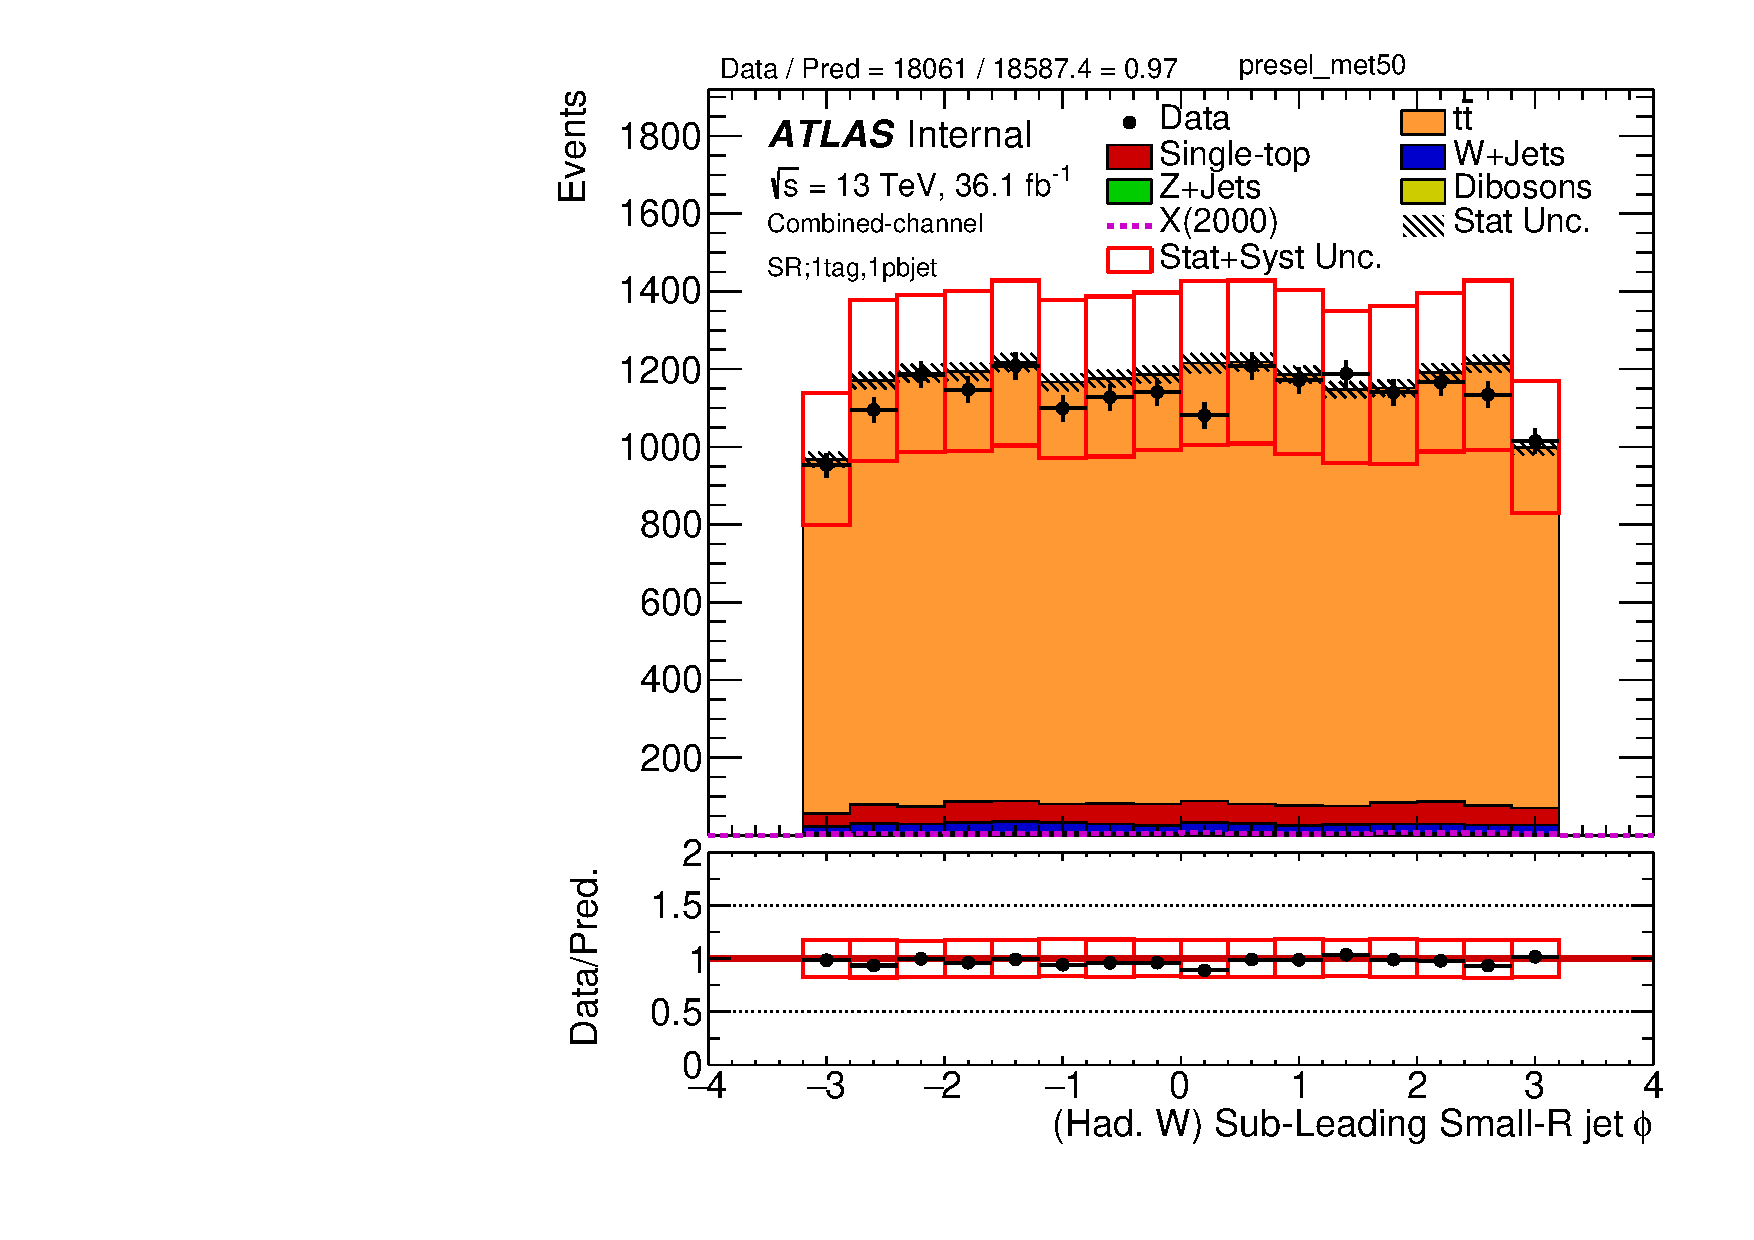
\includegraphics[scale=0.33]{./figures/boosted/Plot1tag1pbjet/DataMC_1tag_1pbjet_SR_lepton_presel_met50_LightJet2Phi}{fig:SR_1tag_1pbjet_jet2_phi}{Sub-leading jet $\phi$}\\
% \caption{Kinematic distributions of the leading and sub-leading small-$R$ jets (of the reconstructed hadronic W) in the 1tag,1pbjet signal region. 
% All plots are prefit.}
% \label{fig:boosted_SR_1tag_1pbjet_whad_jets}
% \end{center}
% \end{figure}

\clearpage
\FloatBarrier

\subsection{\POWHEG+\PYTHIA6 vs \POWHEG+\PYTHIA8 comparison}

The nominal $t\bar{t}$ MC used in this analysis is \POWHEG+\PYTHIA6 (DSID:410000 and 410007). Physics Modelling Group (PMG) 
and Top Working Group recommends the use of \POWHEG+\PYTHIA8 for analysis aiming to be completed in mid-2017. The choice of 
\POWHEG+\PYTHIA6 is historical and the availability of the \POWHEG+\PYTHIA8 sample and the recommended alternative MC samples
to asses the modelling uncertainties of \POWHEG+\PYTHIA8 sample came in too late in the stage of the analysis.

A comparison study between \POWHEG+\PYTHIA6 and \POWHEG+\PYTHIA8 is conducted in order to assess the differences between the two 
samples. The predicted yield between the two samples are similar, as shown in Figure~\ref{fig:boosted_ttbarpy6py8_yield}. 
Figure~\ref{fig:boosted_ttbarpy6py8_hhMass}-~\ref{fig:boosted_ttbarpy6py8_WlepMtATLAS} 
compares \POWHEG+\PYTHIA6  and \POWHEG+\PYTHIA8 prediction of the $t\bar{t}$ in the 2-tag signal region with modelling systematic 
uncertainties for \POWHEG+\PYTHIA6  from four different sources as described in Section~\ref{sec:boosted_syst_modelling_top}. 
No significant difference is observed between \POWHEG+\PYTHIA6 and \POWHEG+\PYTHIA8.


\begin{figure}[!h]
\begin{center}
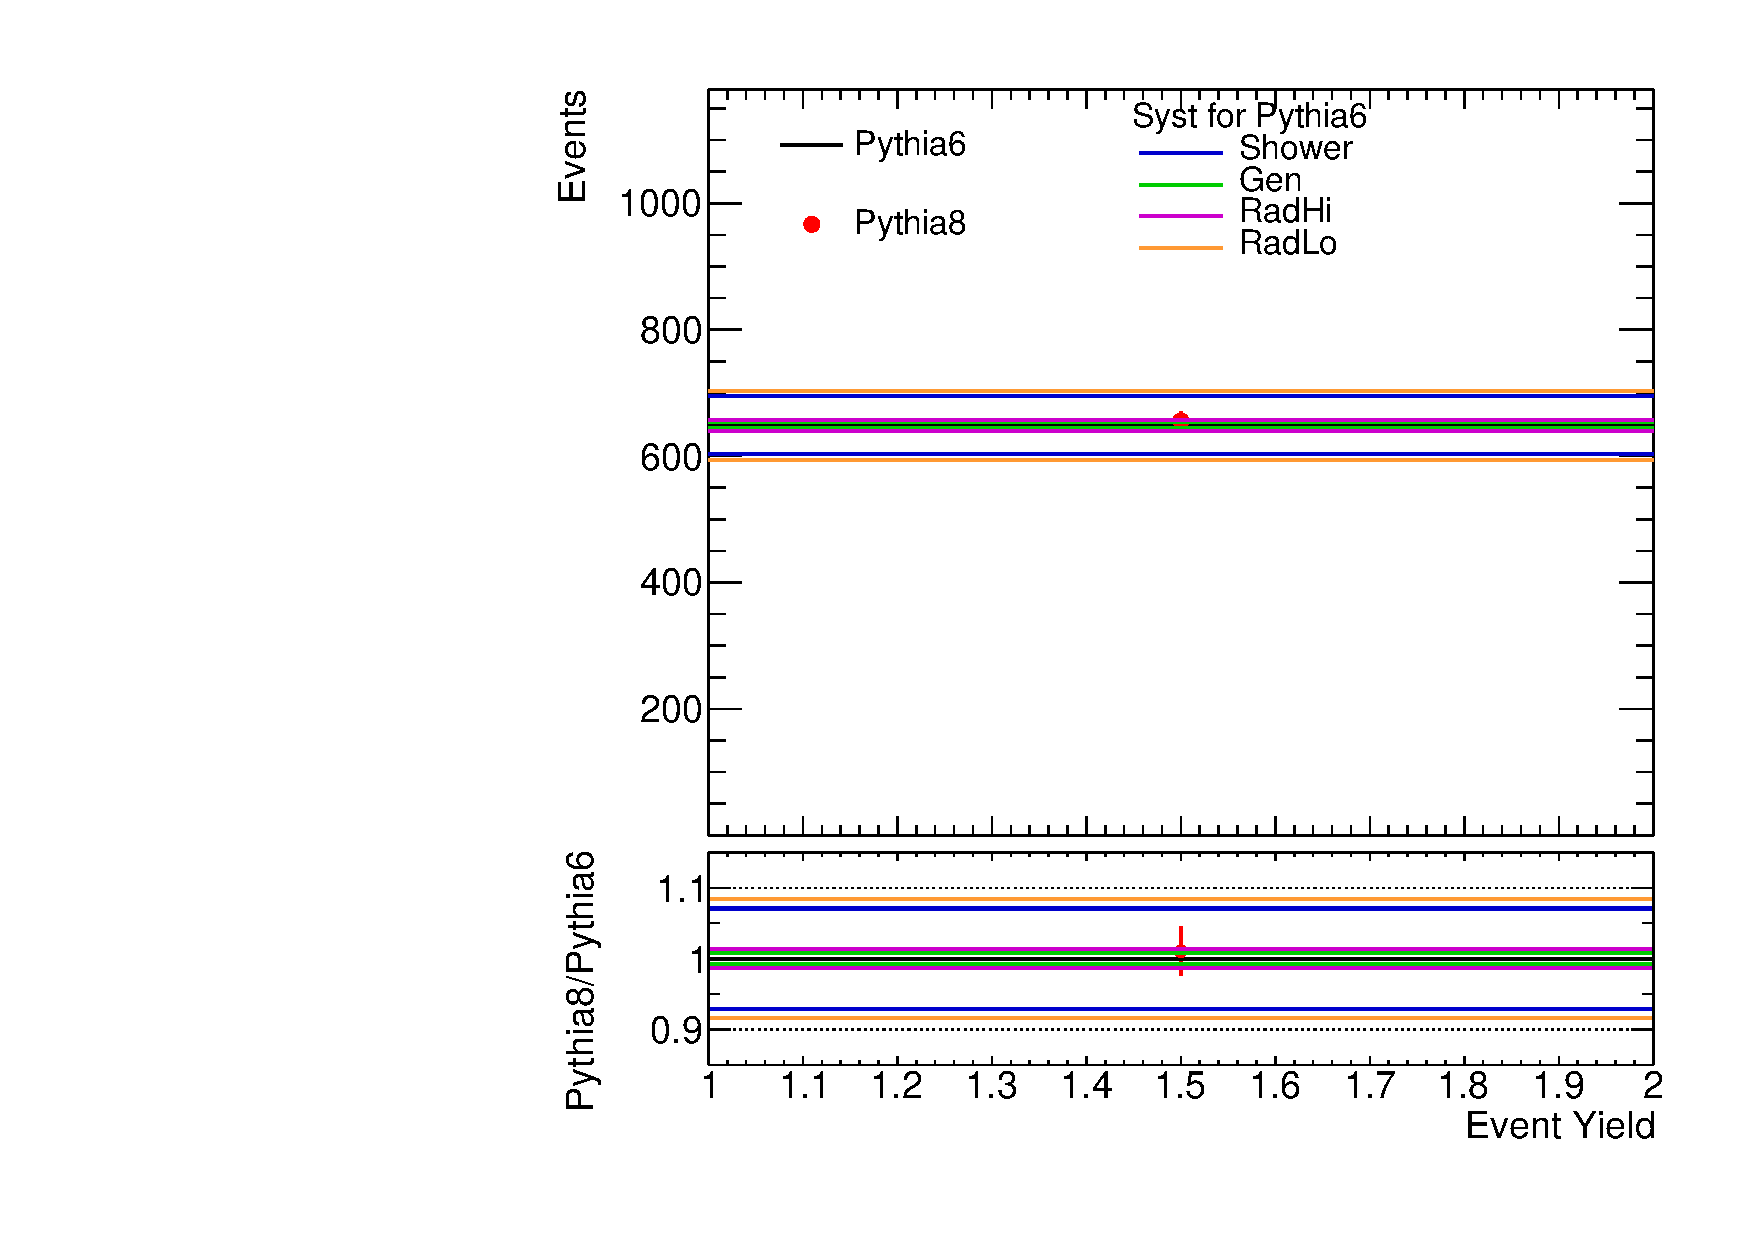
\includegraphics[scale=0.33]{./figures/boosted/TTBarPy6VsPy8/TTBarPy6VsPy8_SR_neventsweighted_all} 
\caption{One bin distribution representing the yield in the 2-tag signal region, where the predicted yield of Powheg+Pythia6 and Powheg+Pythia8 $t\bar{t}$ MC
are compared. The systematic variations for Powheg+Pythia6 are also shown.}
\label{fig:boosted_ttbarpy6py8_yield}
\end{center}
\end{figure}


\begin{figure}[!h]
\begin{center}
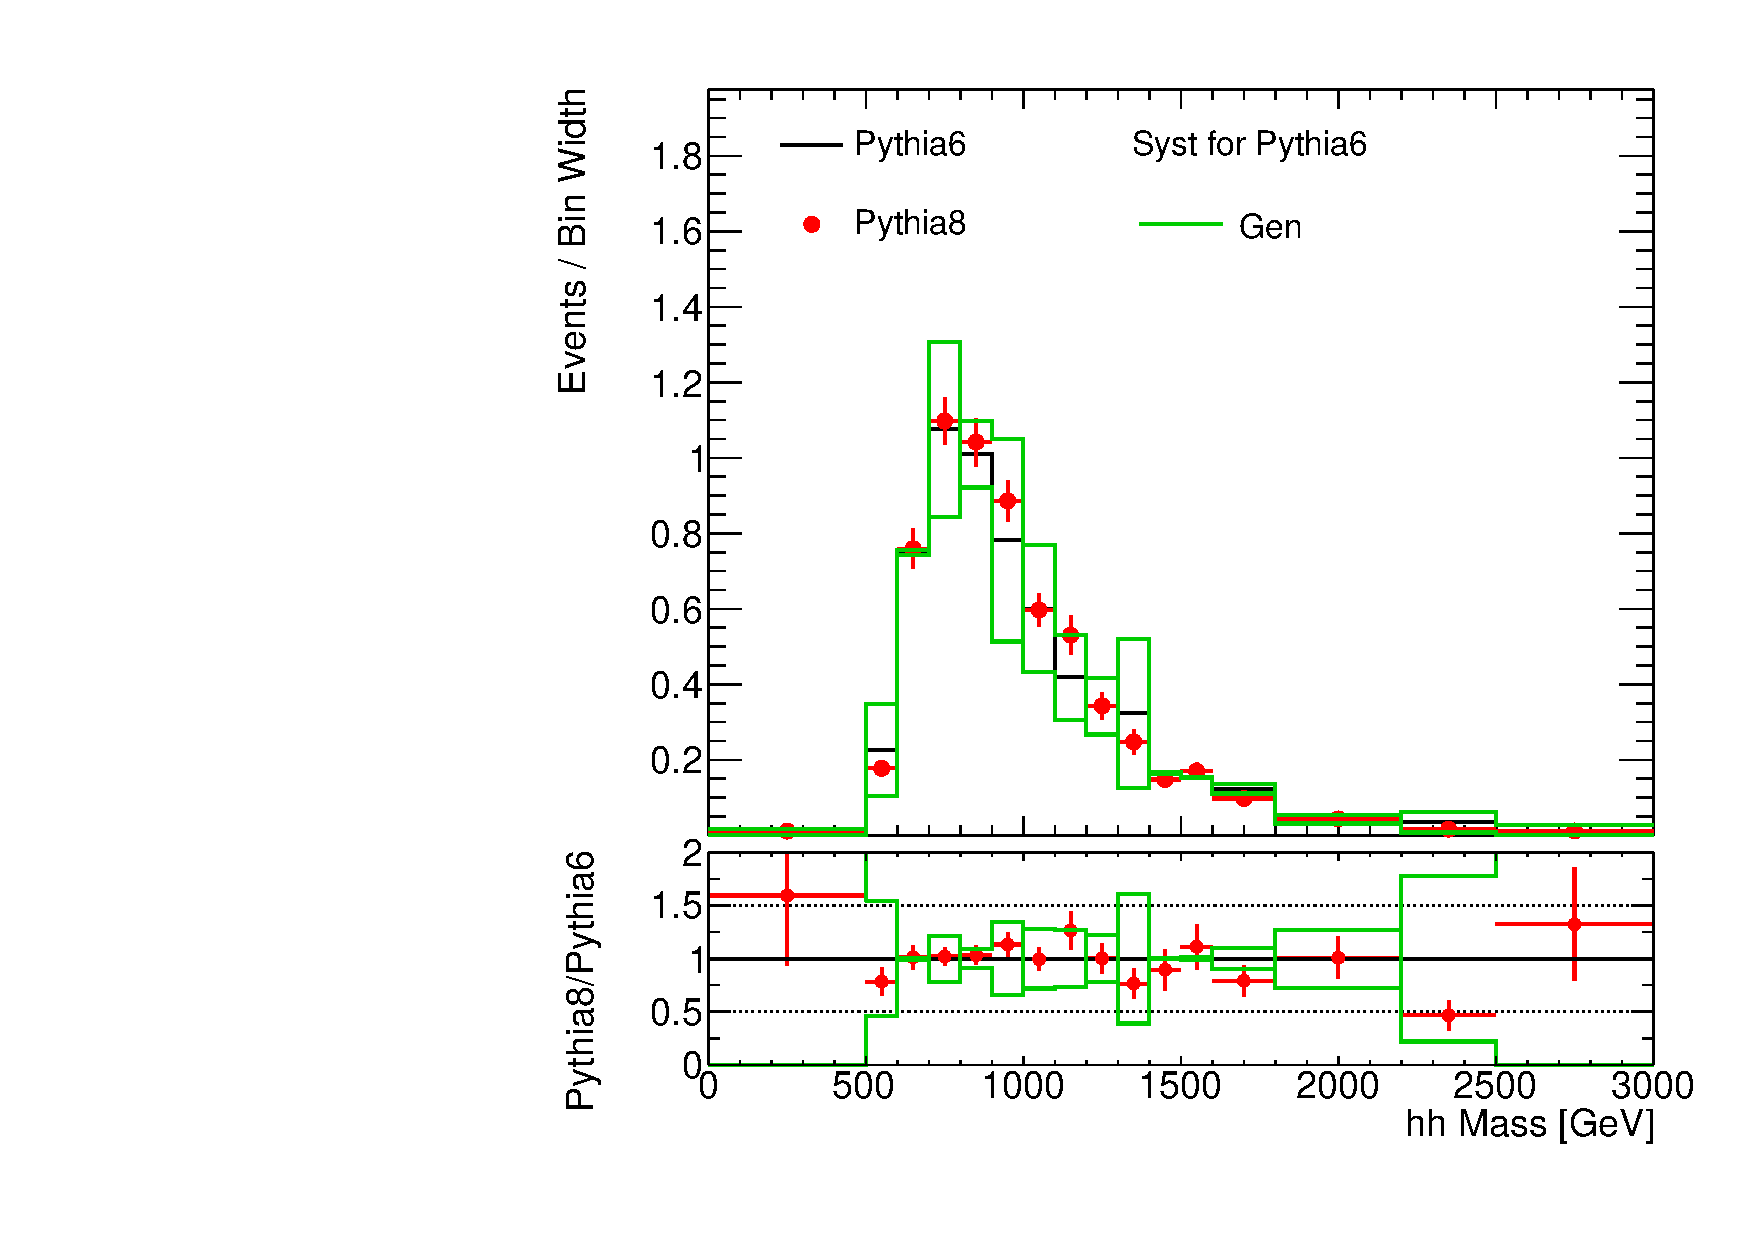
\includegraphics[scale=0.33]{./figures/boosted/TTBarPy6VsPy8/TTBarPy6VsPy8_SR_hhMassRebin1_gen}  
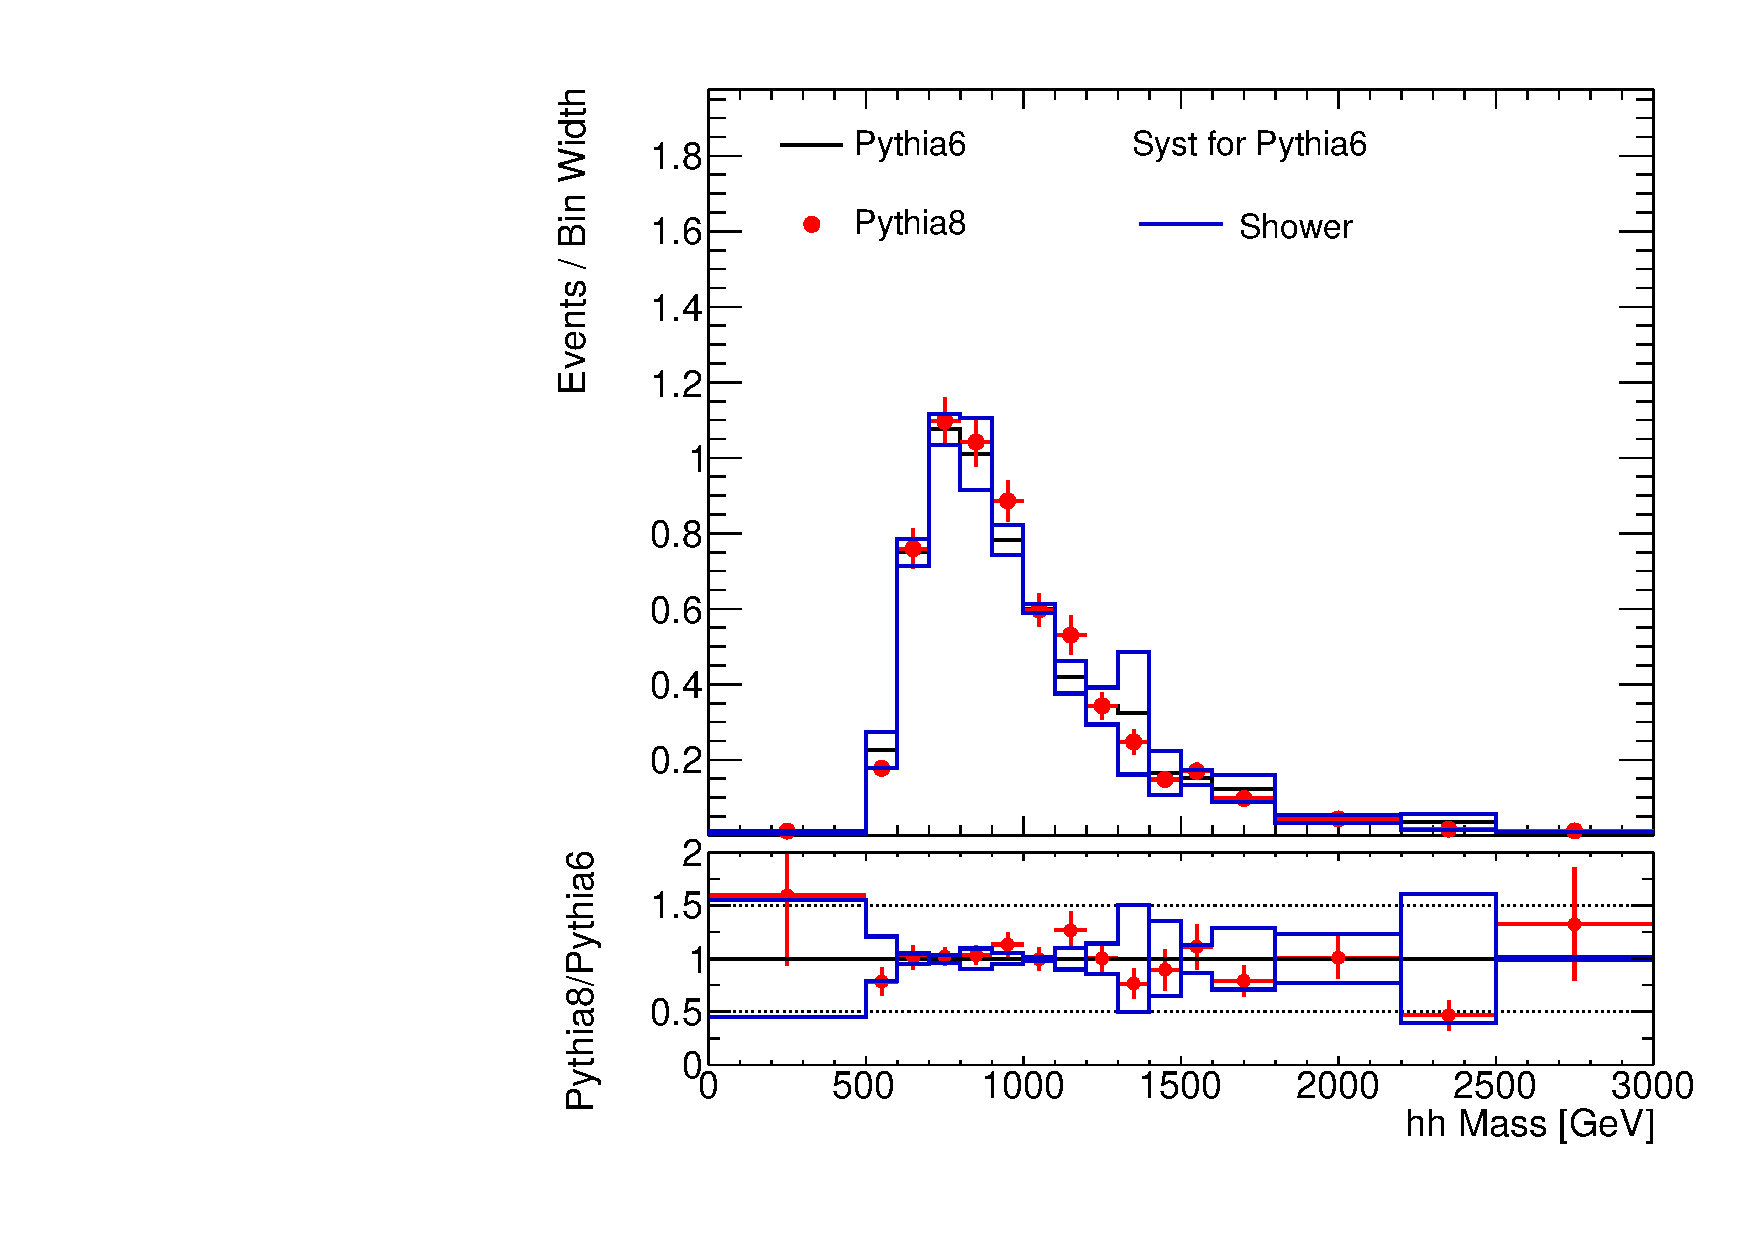
\includegraphics[scale=0.33]{./figures/boosted/TTBarPy6VsPy8/TTBarPy6VsPy8_SR_hhMassRebin1_shower} \\
\par\medskip
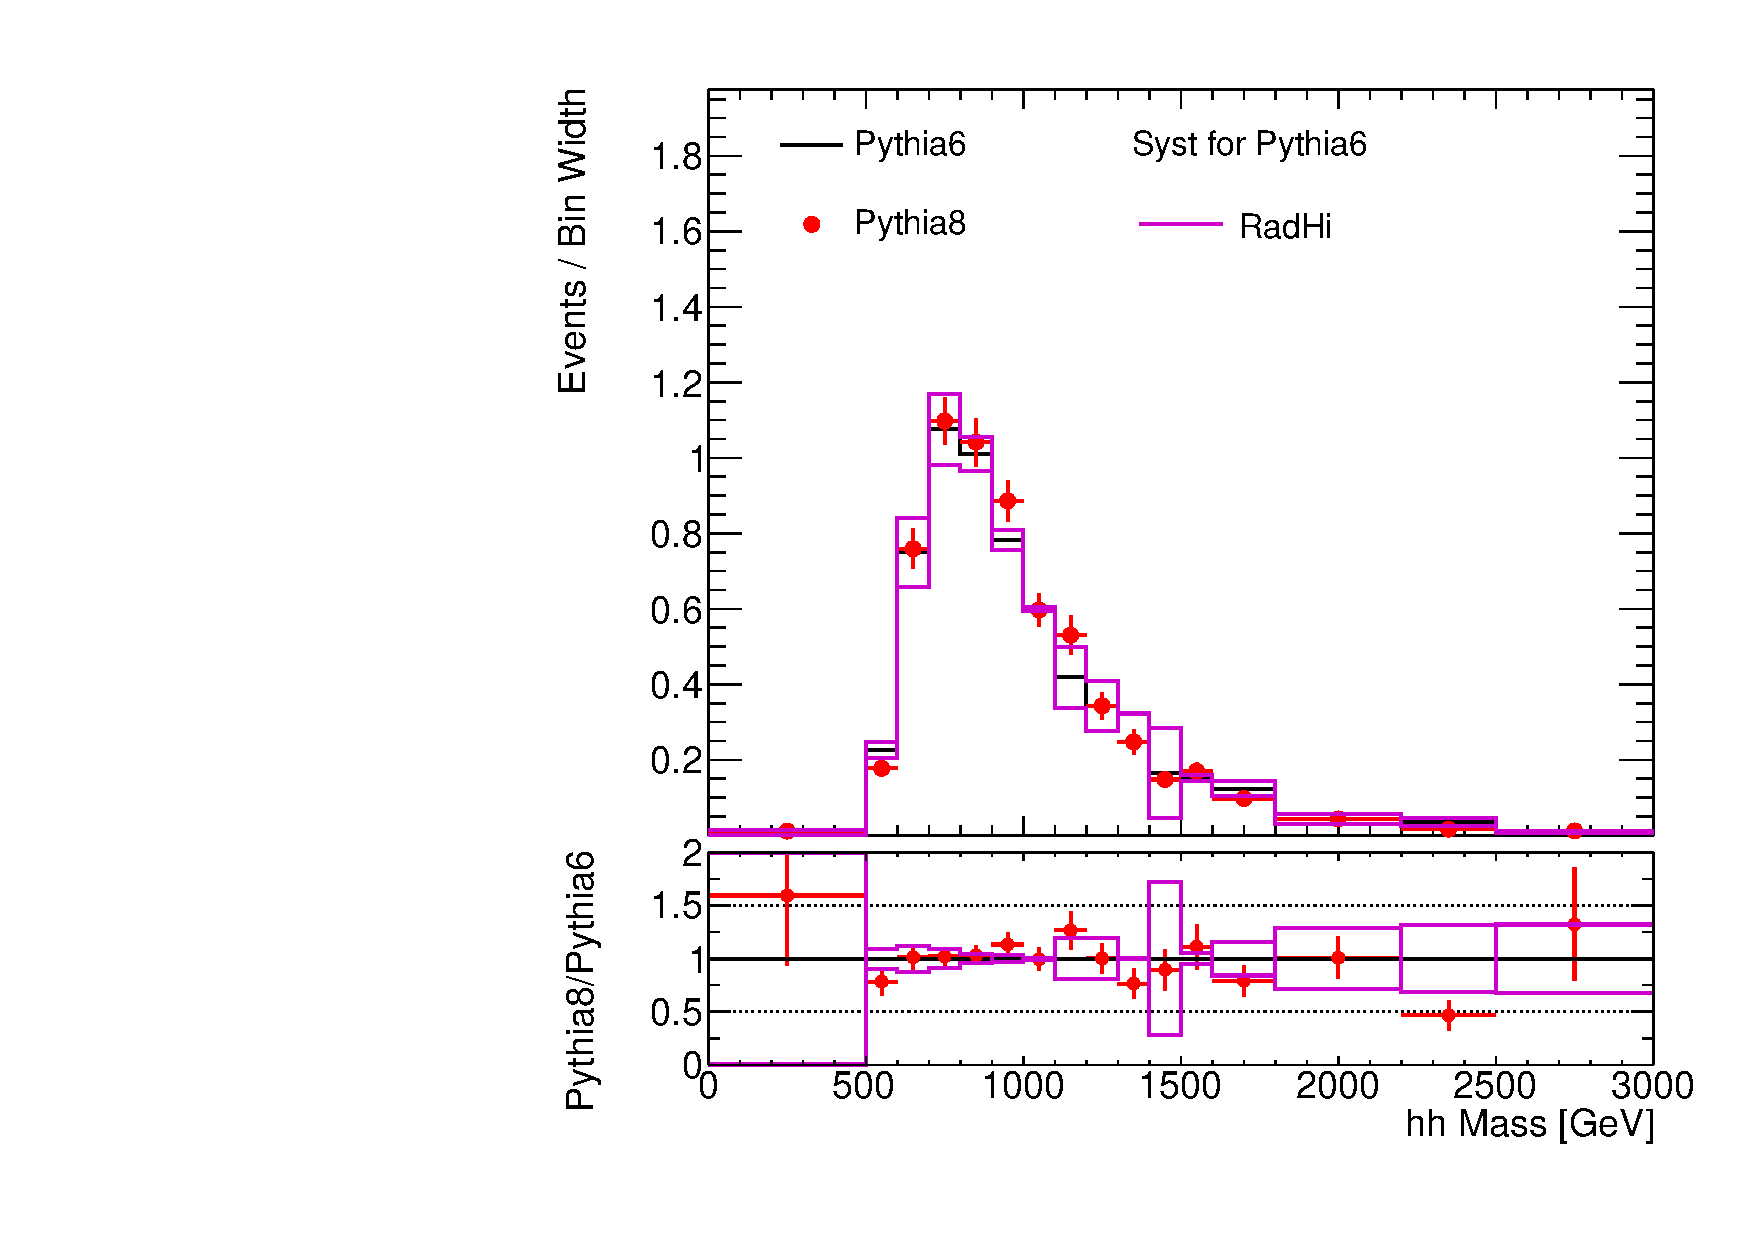
\includegraphics[scale=0.33]{./figures/boosted/TTBarPy6VsPy8/TTBarPy6VsPy8_SR_hhMassRebin1_radhi}
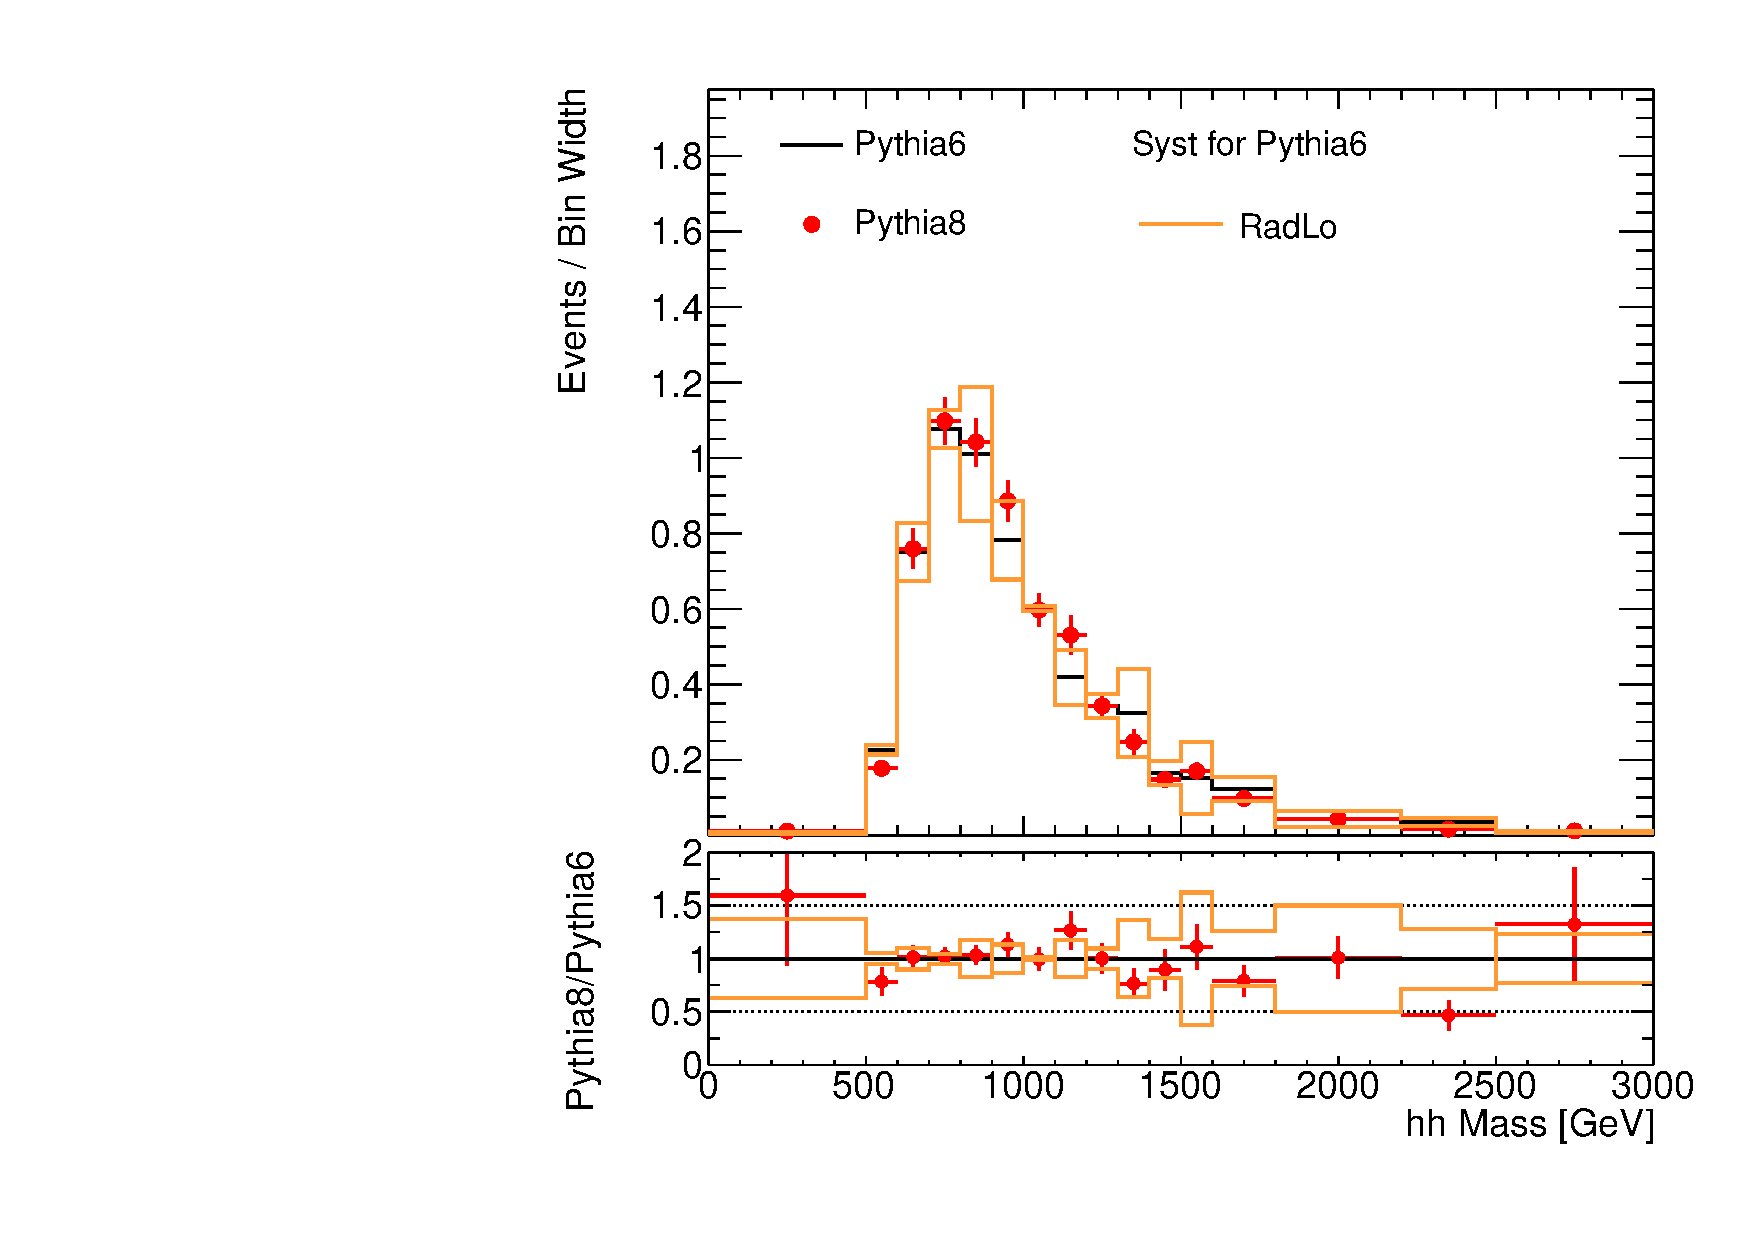
\includegraphics[scale=0.33]{./figures/boosted/TTBarPy6VsPy8/TTBarPy6VsPy8_SR_hhMassRebin1_radlo}
\caption{$m_{hh}$ distribution, in the 2-tag signal region, comparisons between Powheg+Pythia6 and Powheg+Pythia8 $t\bar{t}$ MC. 
The systematic variation for Powheg+Pythia6 is shown in each plot.}
\label{fig:boosted_ttbarpy6py8_hhMass}
\end{center}
\end{figure}

\begin{figure}[!h]
\begin{center}
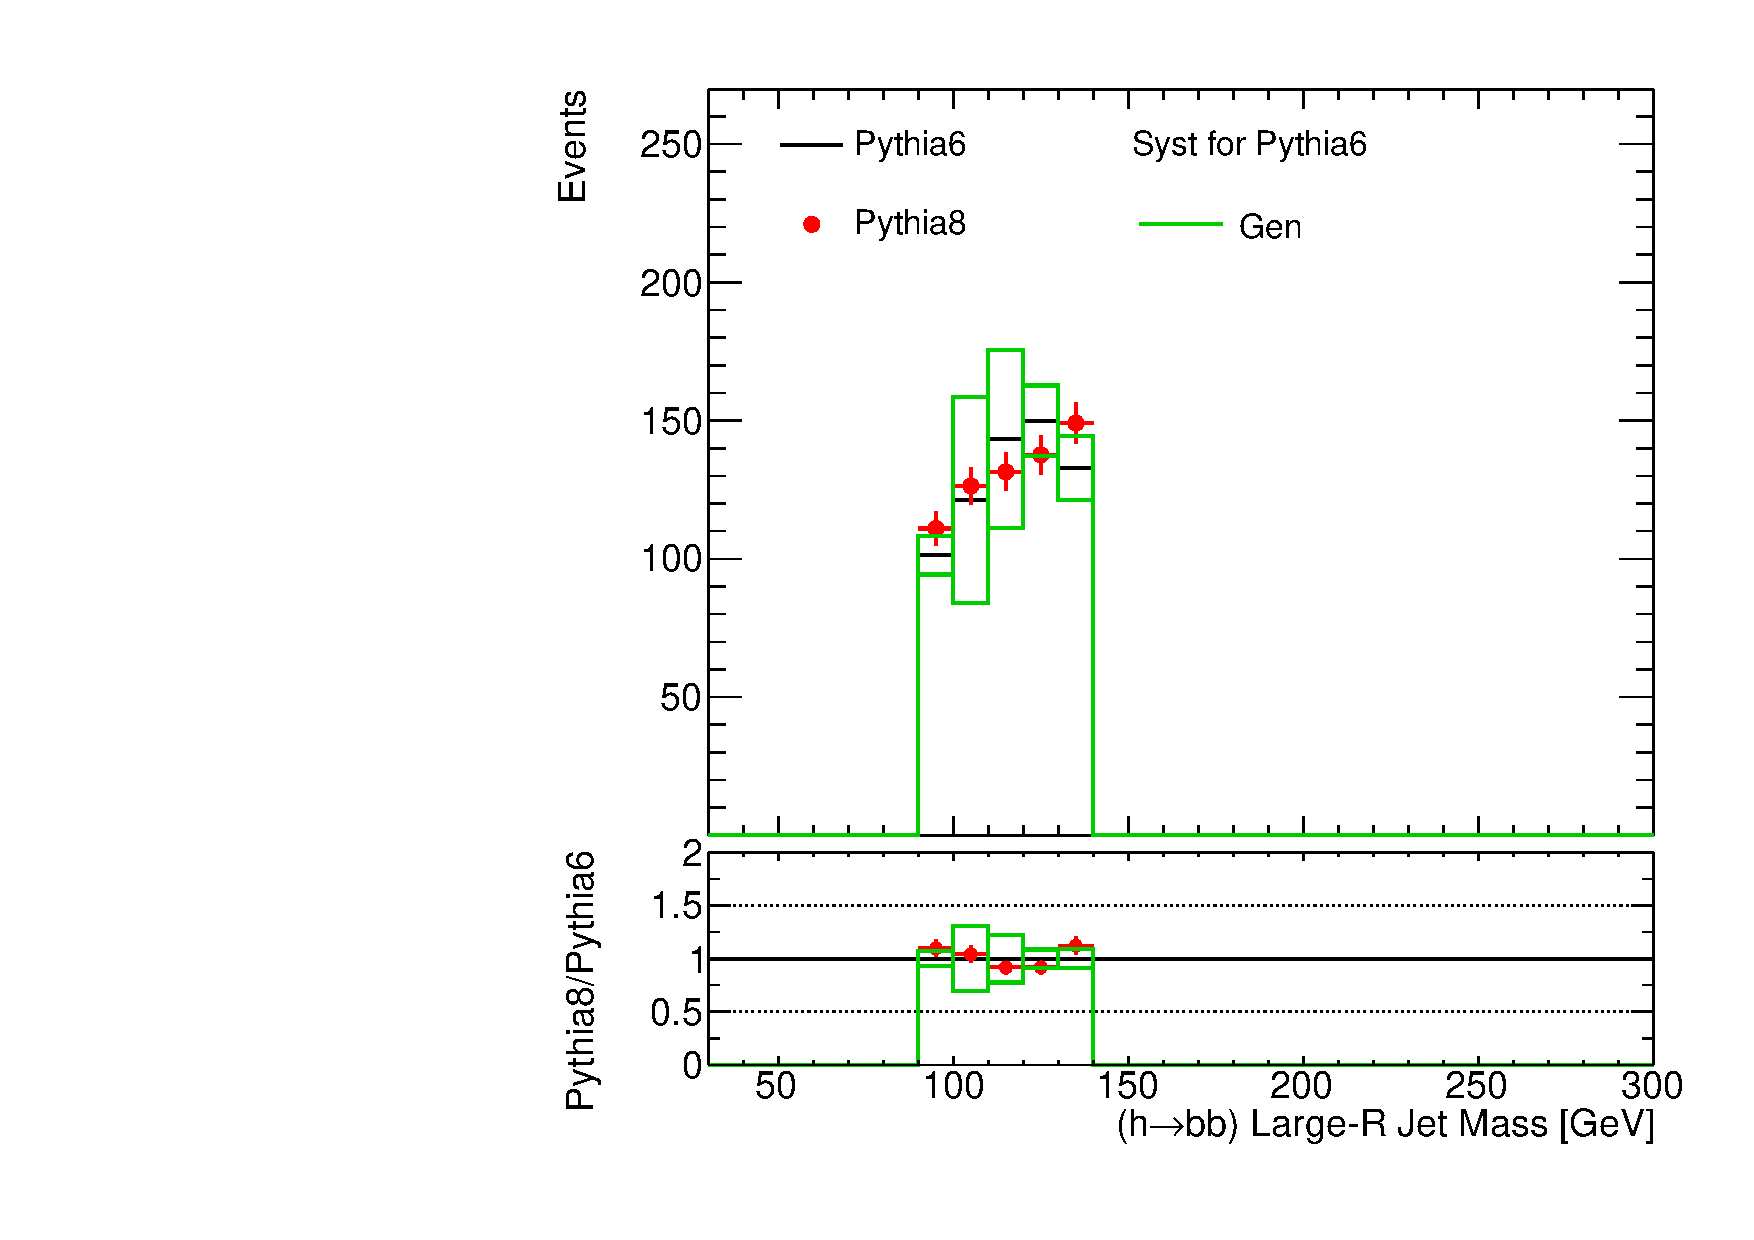
\includegraphics[scale=0.33]{./figures/boosted/TTBarPy6VsPy8/TTBarPy6VsPy8_SR_HbbMass_gen}   
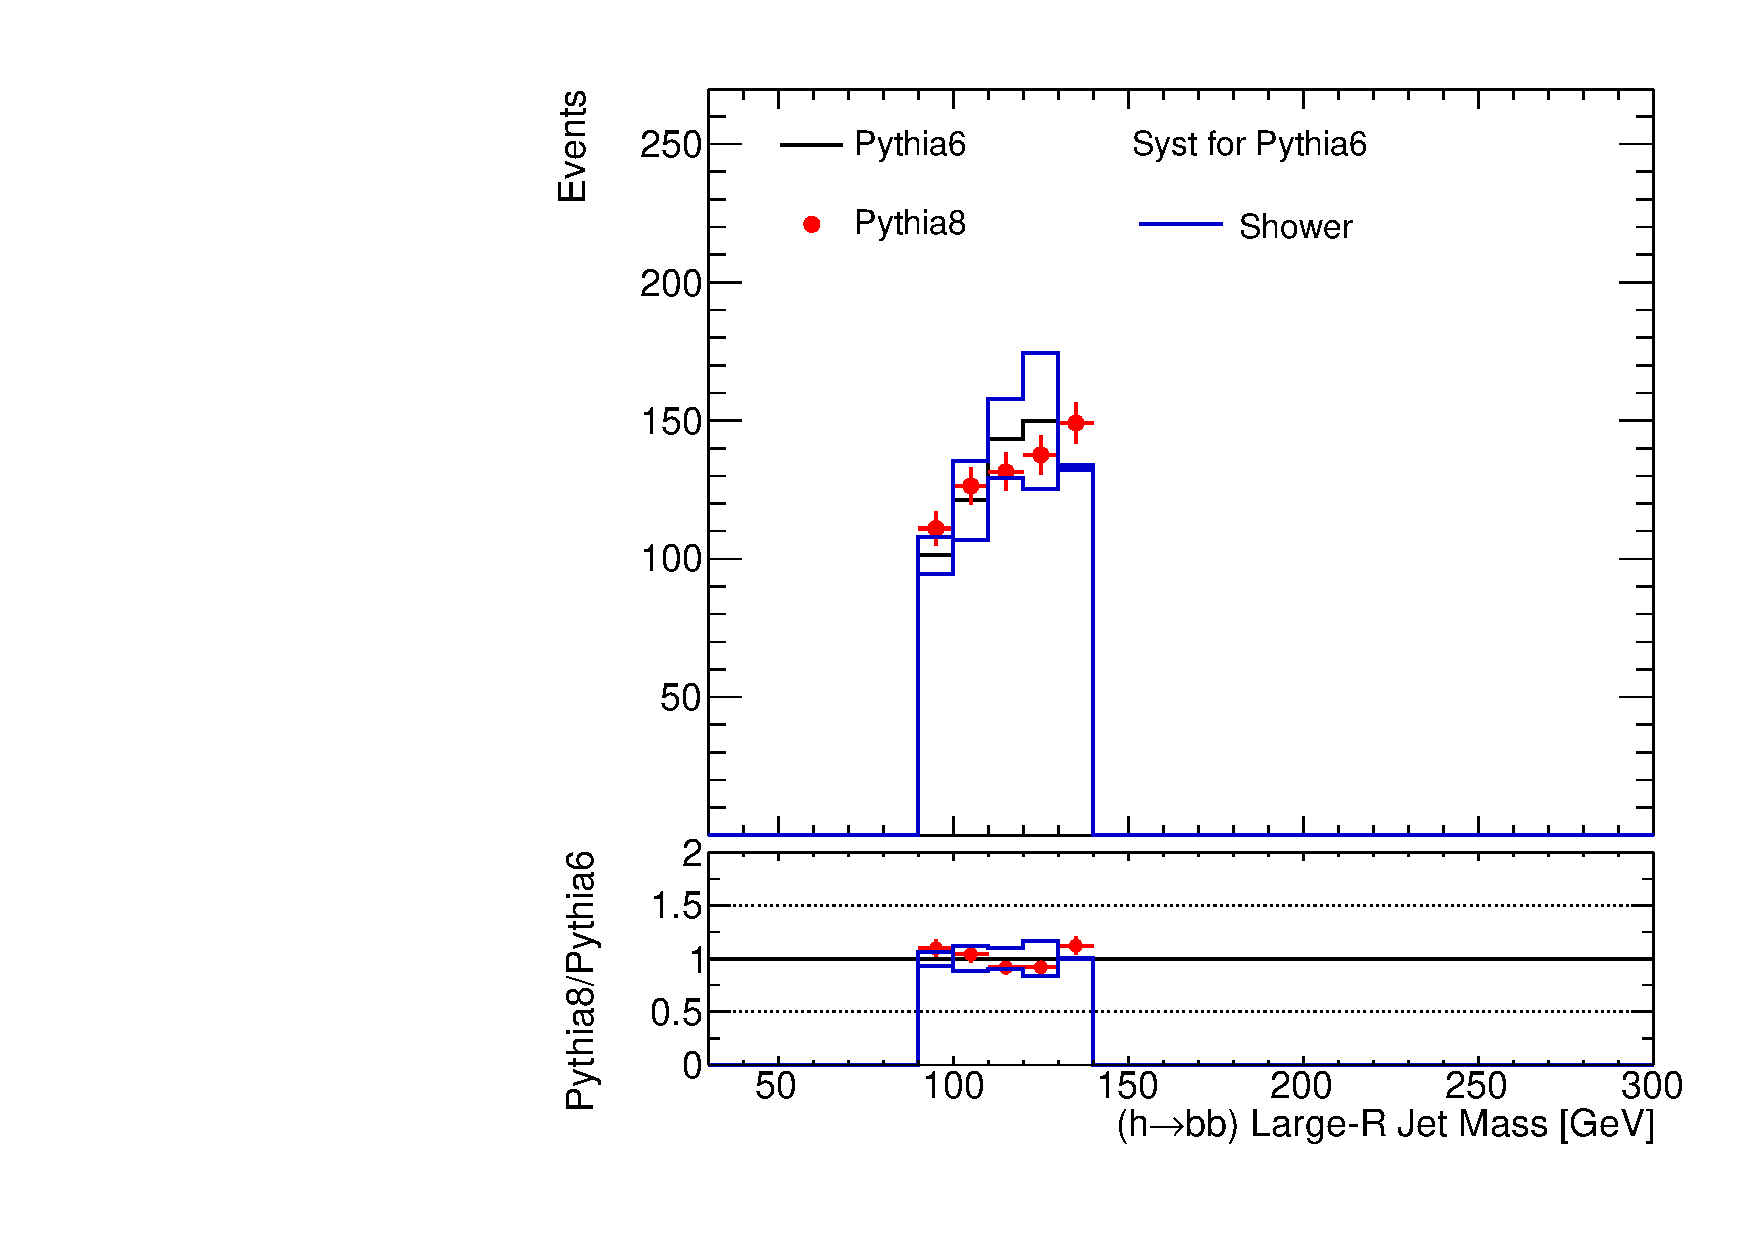
\includegraphics[scale=0.33]{./figures/boosted/TTBarPy6VsPy8/TTBarPy6VsPy8_SR_HbbMass_shower} \\
\par\medskip
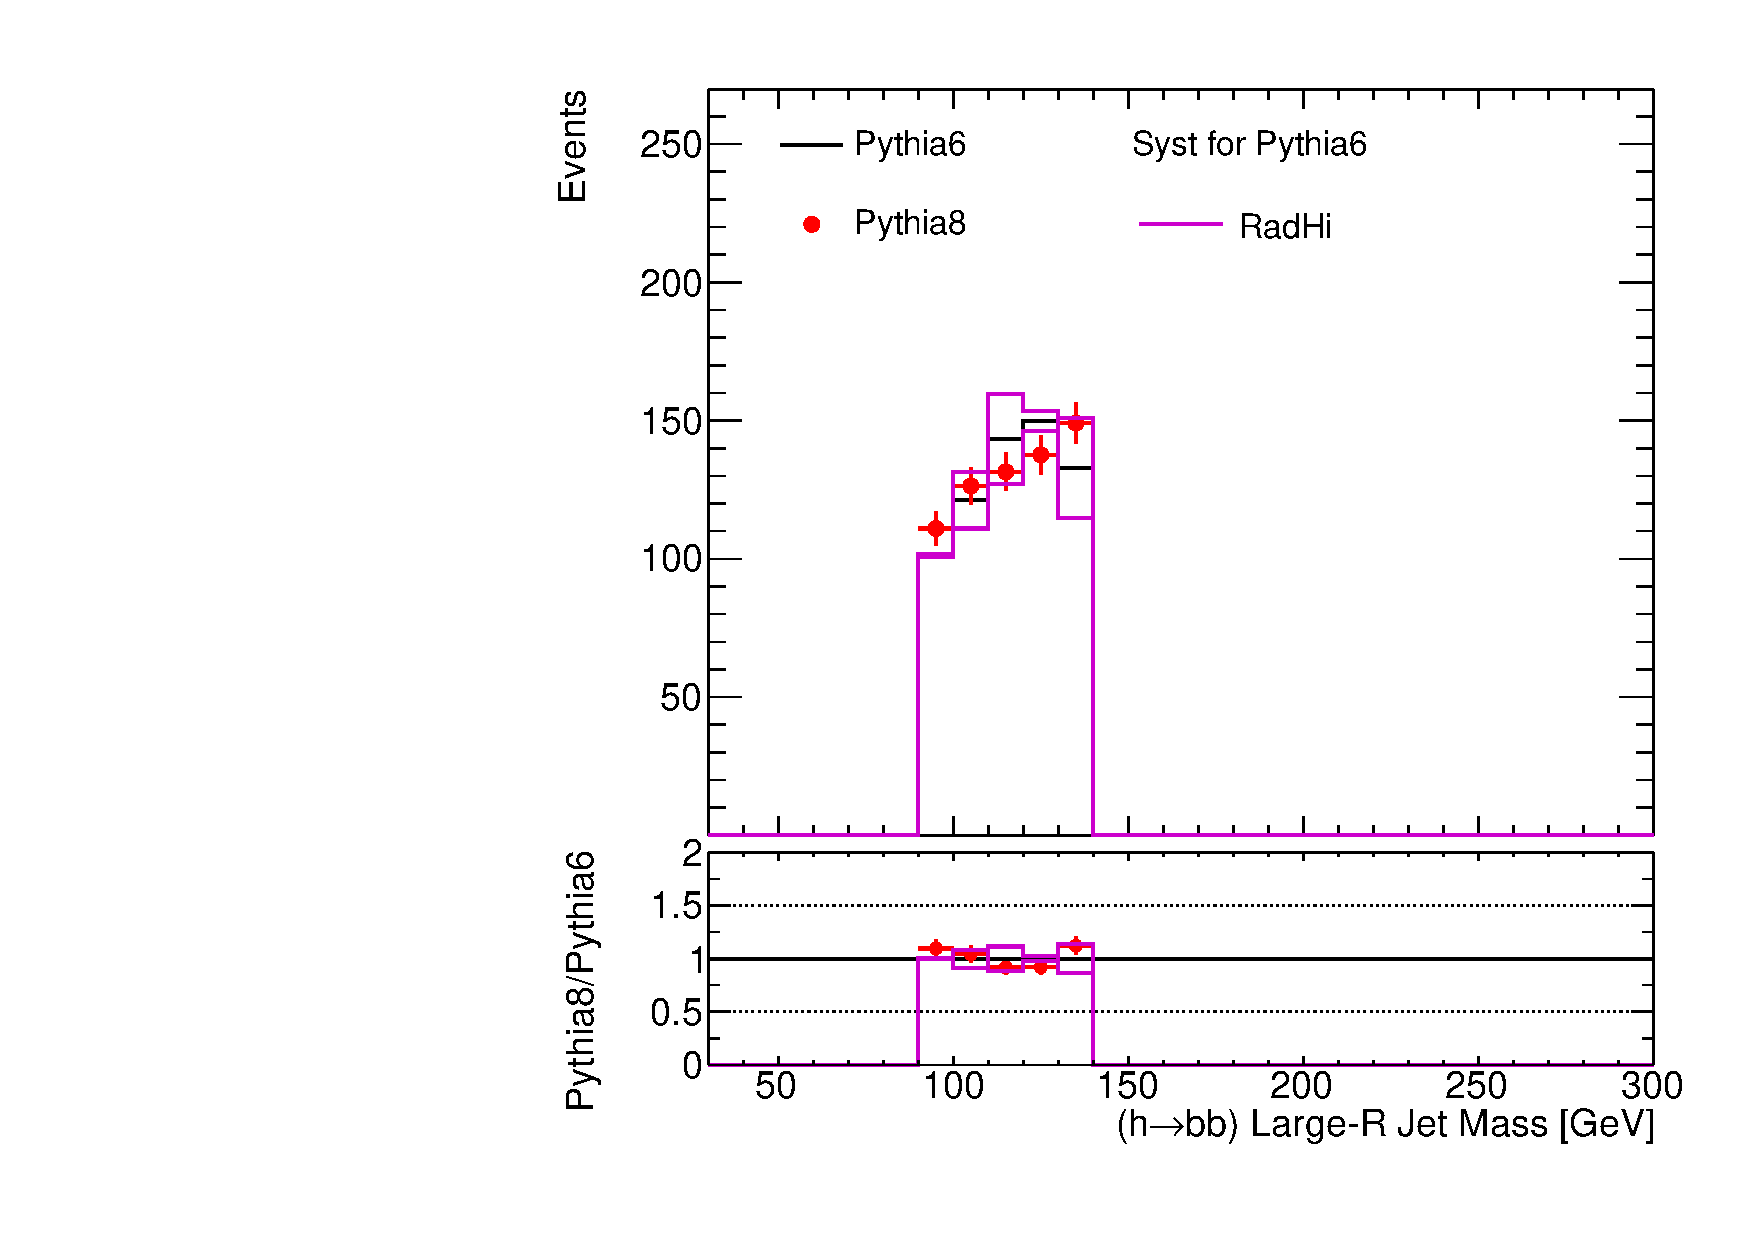
\includegraphics[scale=0.33]{./figures/boosted/TTBarPy6VsPy8/TTBarPy6VsPy8_SR_HbbMass_radhi}
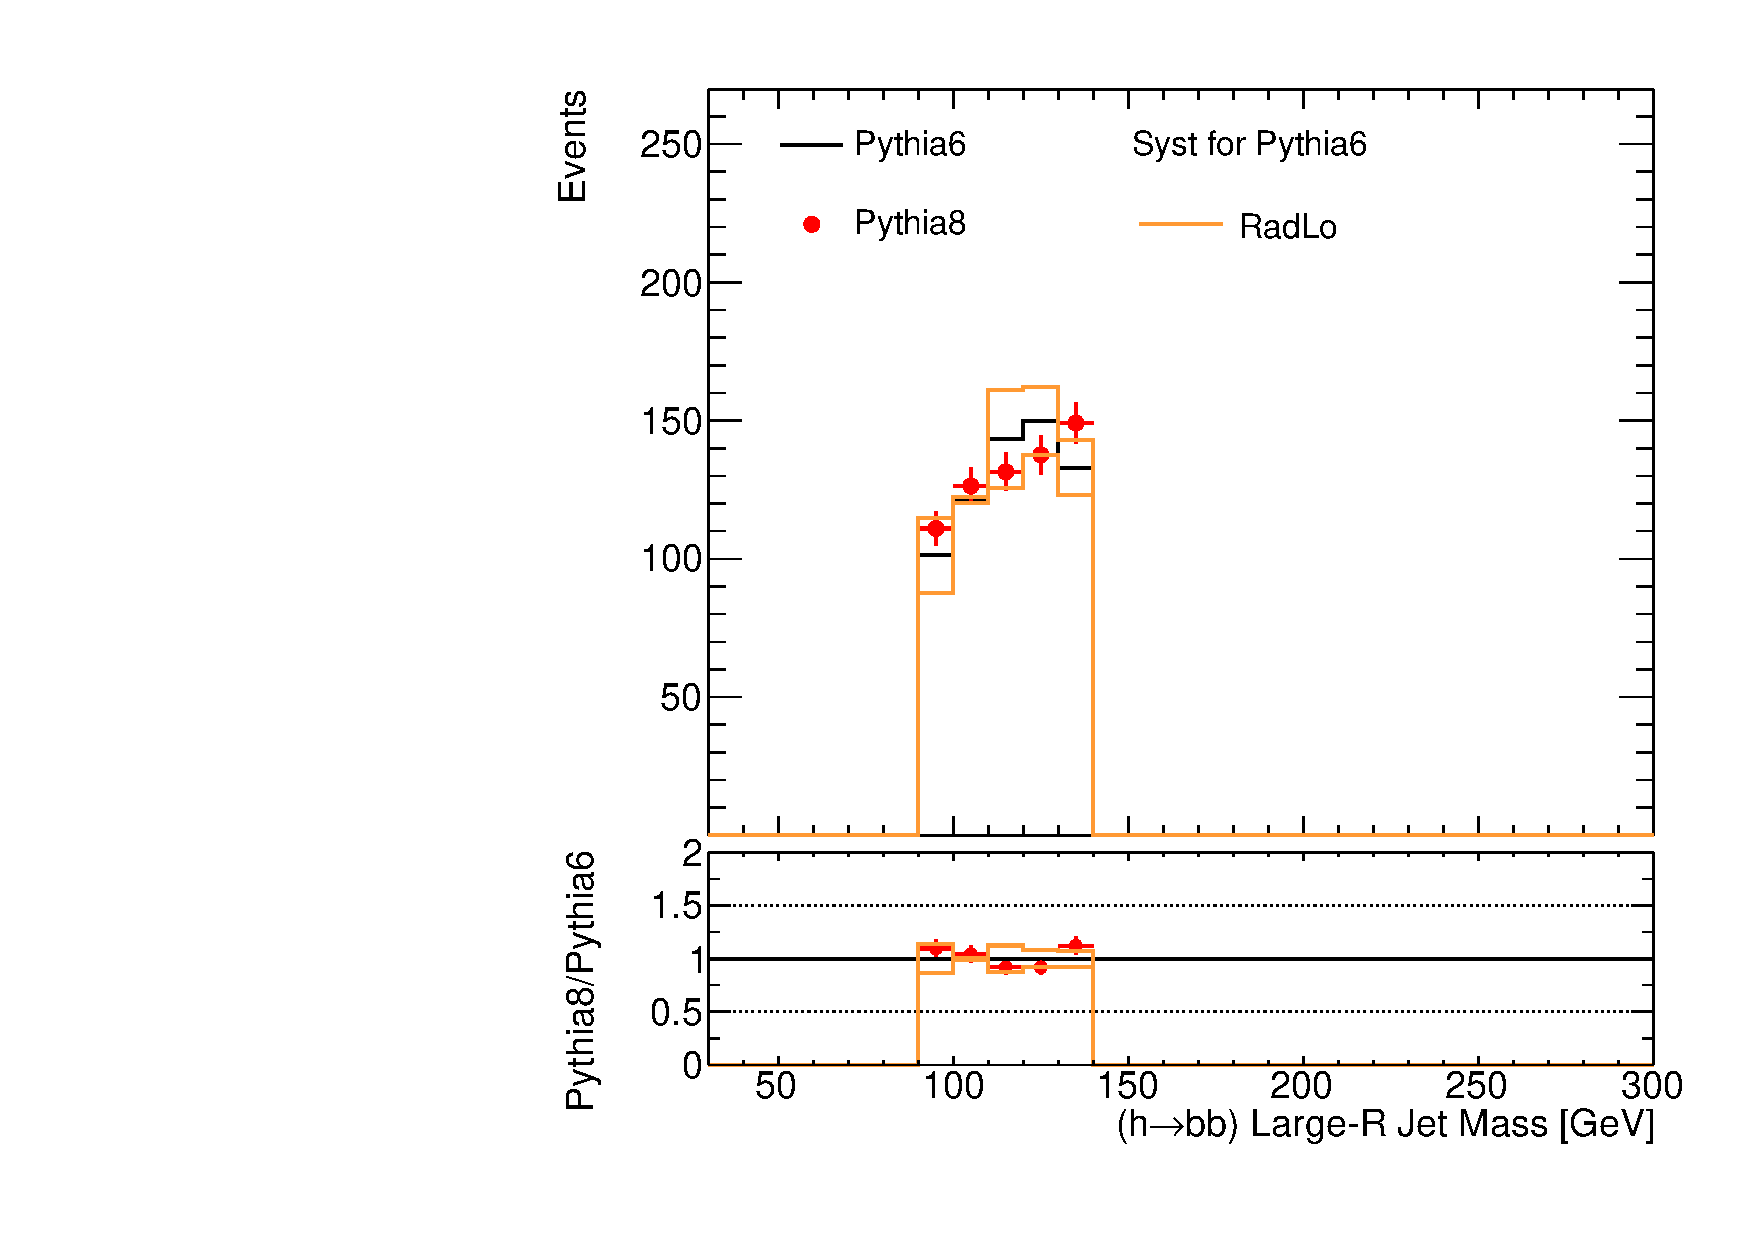
\includegraphics[scale=0.33]{./figures/boosted/TTBarPy6VsPy8/TTBarPy6VsPy8_SR_HbbMass_radlo}
\caption{Large-$R$ jet mass distribution, in the 2-tag signal region, comparisons between Powheg+Pythia6 and Powheg+Pythia8 $t\bar{t}$ MC. 
The systematic variation for Powheg+Pythia6 is shown in each plot.}
\label{fig:boosted_ttbarpy6py8_HbbMass}
\end{center}
\end{figure}

\begin{figure}[!h]
\begin{center}
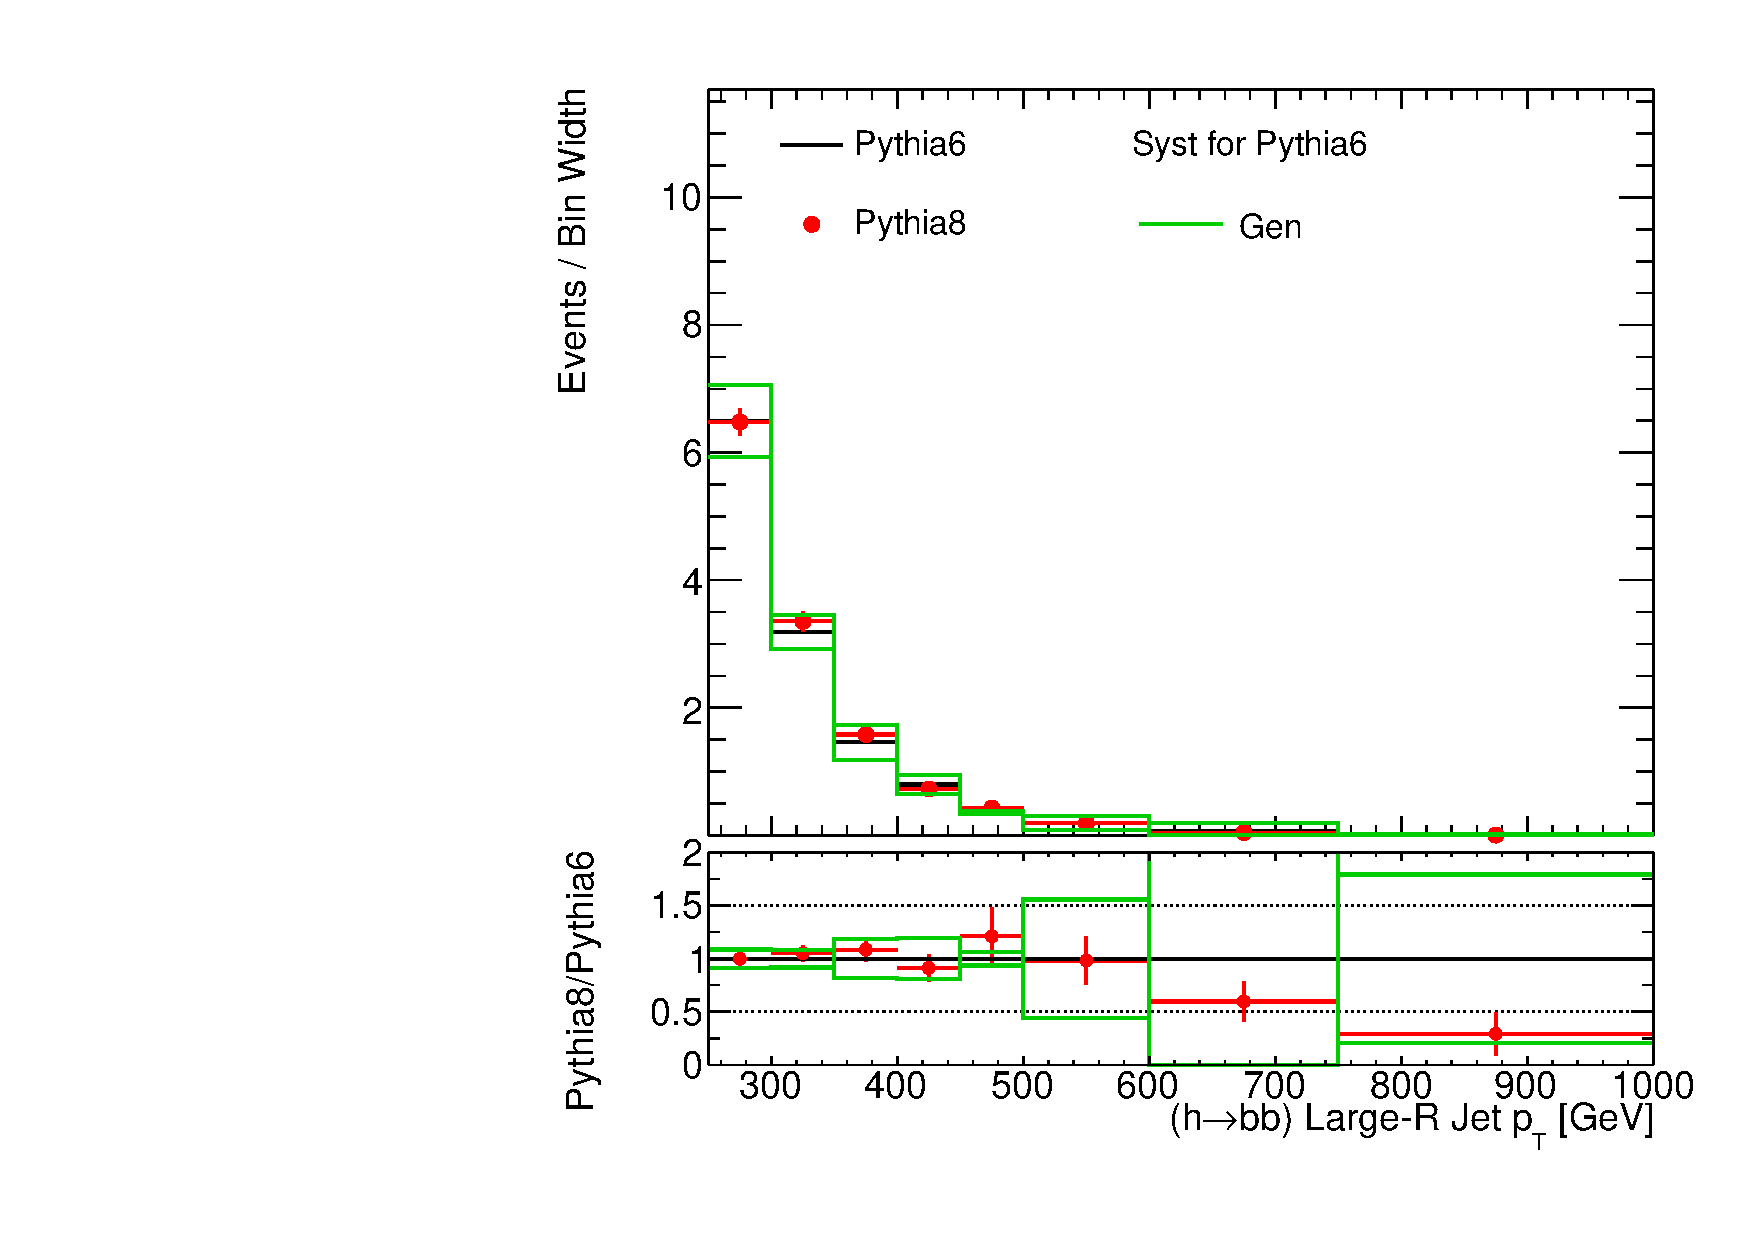
\includegraphics[scale=0.33]{./figures/boosted/TTBarPy6VsPy8/TTBarPy6VsPy8_SR_HbbPt_gen} 
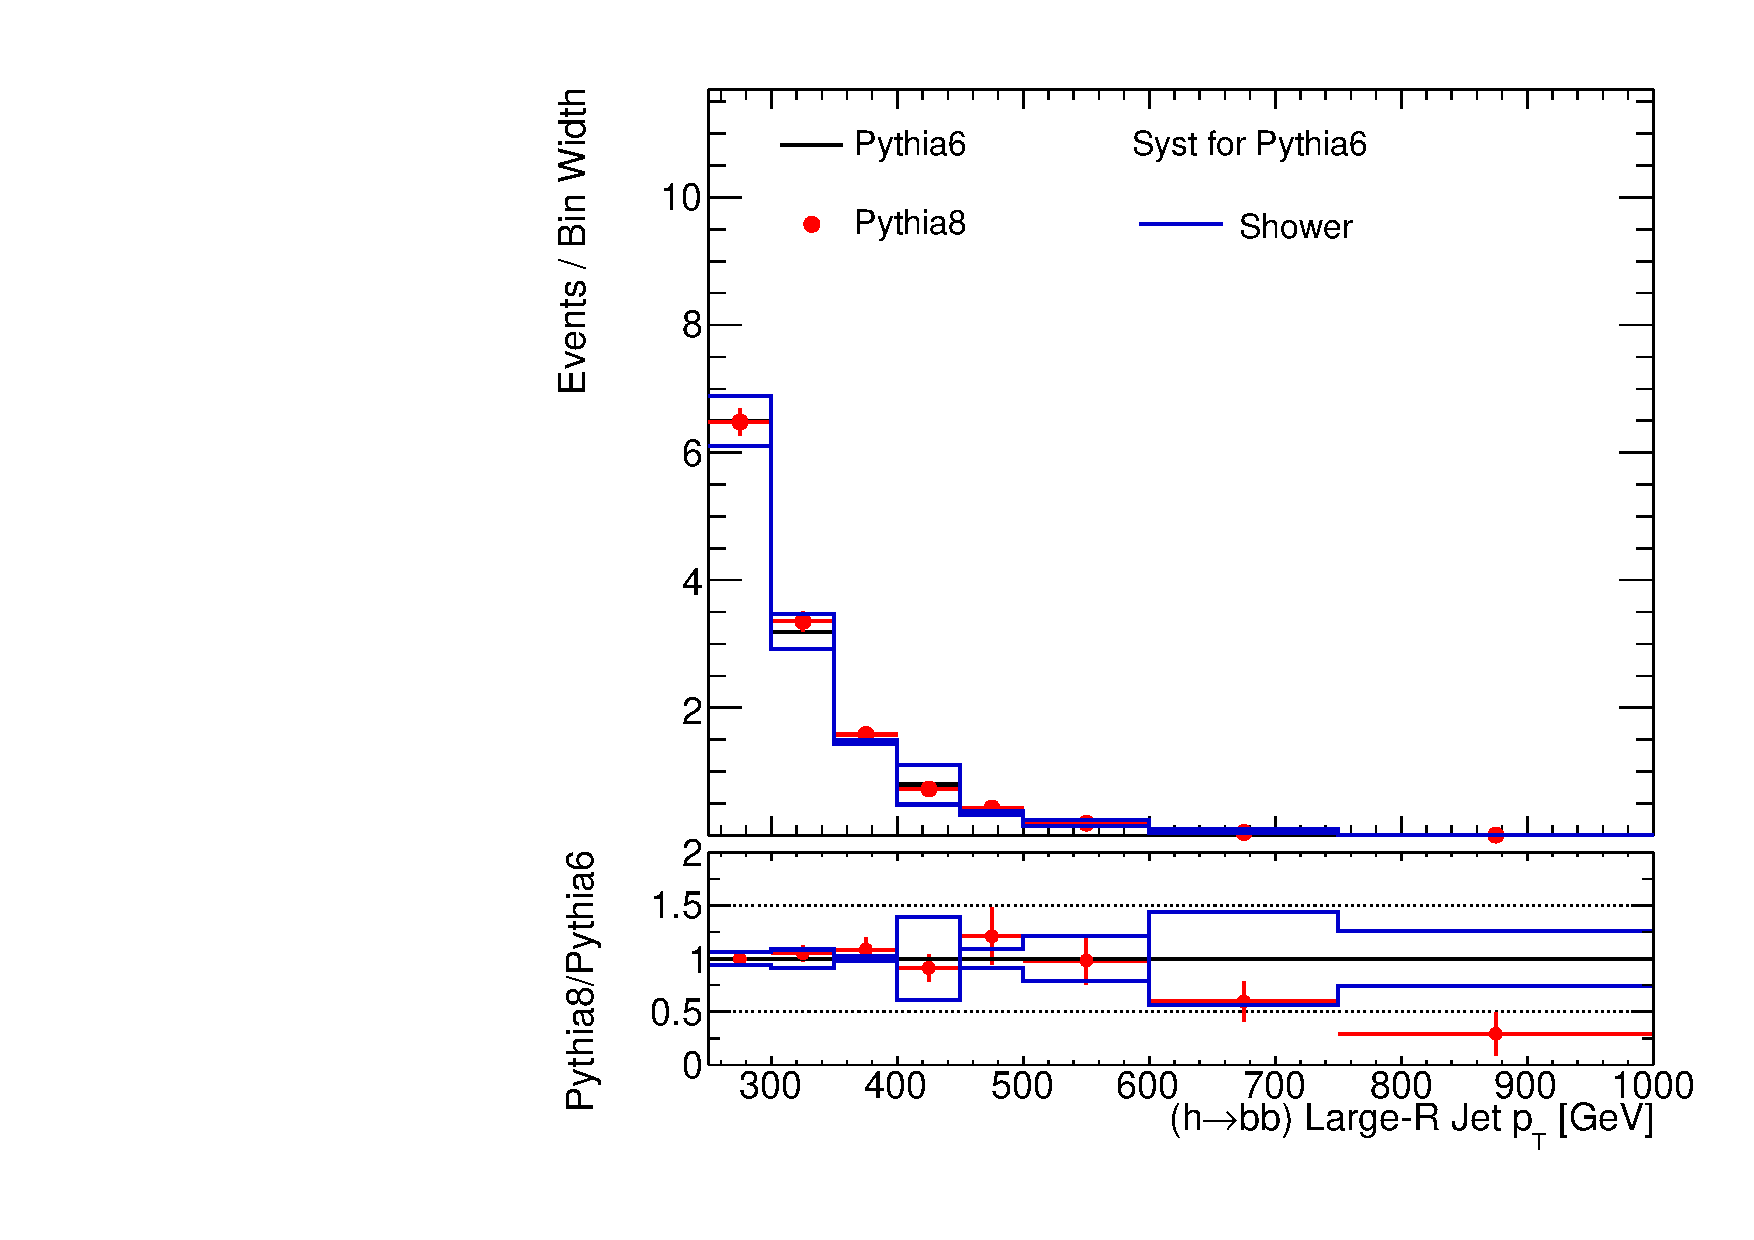
\includegraphics[scale=0.33]{./figures/boosted/TTBarPy6VsPy8/TTBarPy6VsPy8_SR_HbbPt_shower} \\
\par\medskip
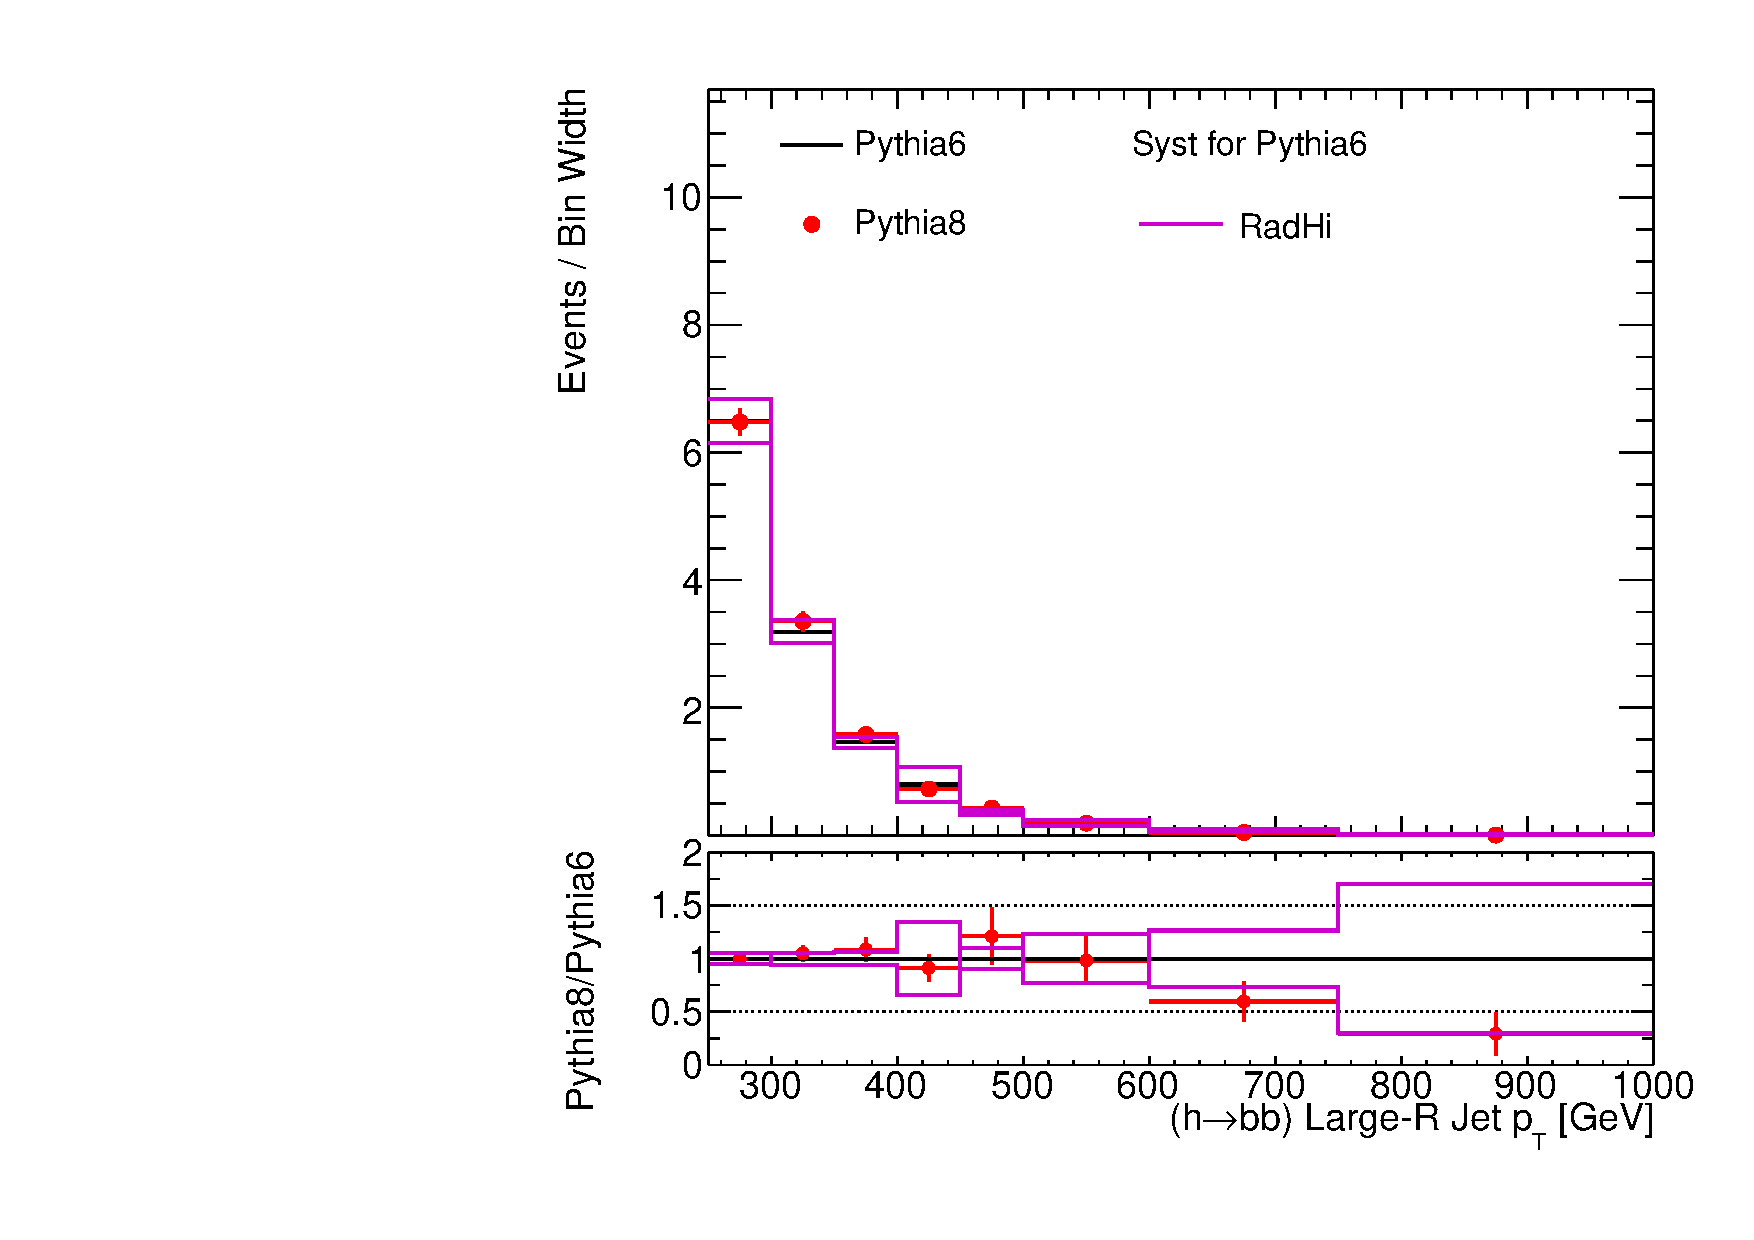
\includegraphics[scale=0.33]{./figures/boosted/TTBarPy6VsPy8/TTBarPy6VsPy8_SR_HbbPt_radhi} 
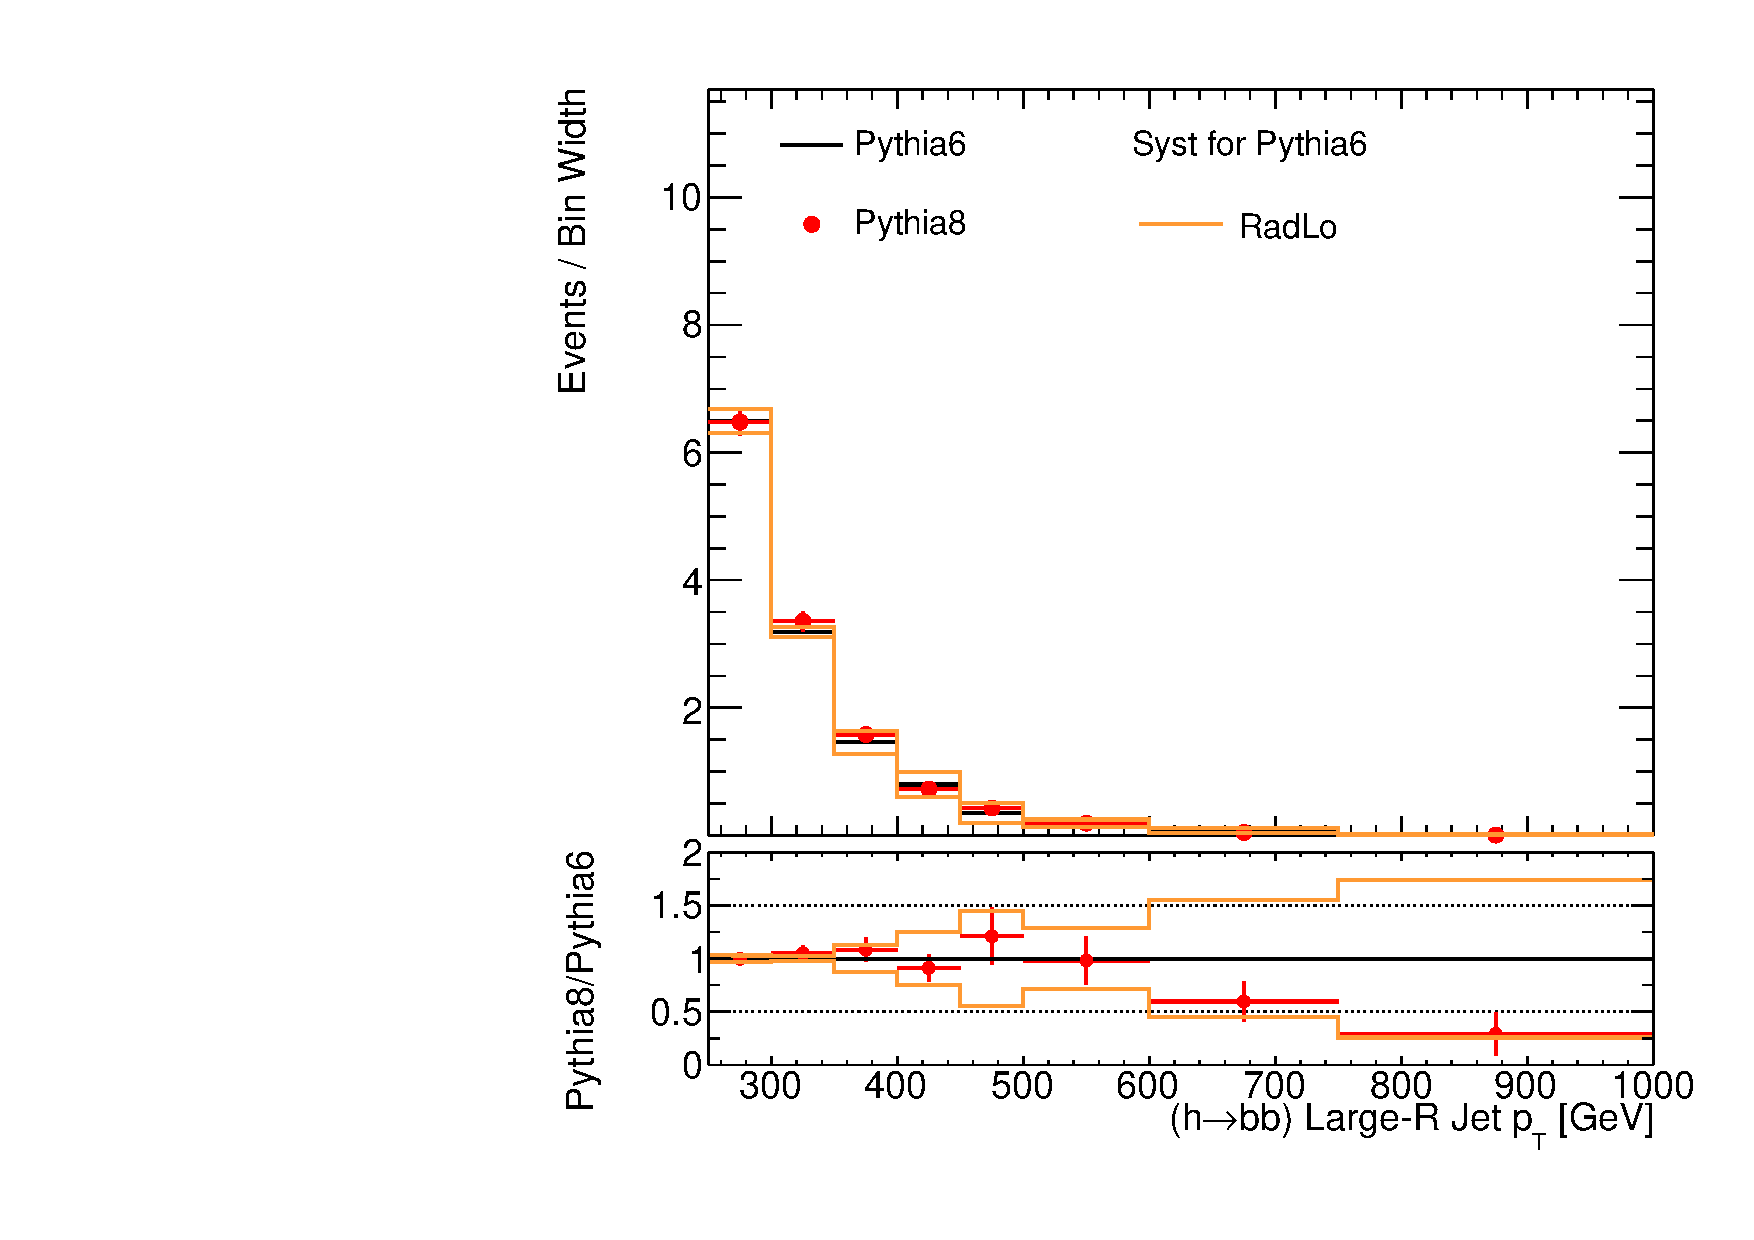
\includegraphics[scale=0.33]{./figures/boosted/TTBarPy6VsPy8/TTBarPy6VsPy8_SR_HbbPt_radlo}
\caption{Large-$R$ jet \pt distribution, in the 2-tag signal region, comparisons between Powheg+Pythia6 and Powheg+Pythia8 $t\bar{t}$ MC. 
The systematic variation for Powheg+Pythia6 is shown in each plot.}
\label{fig:boosted_ttbarpy6py8_HbbPt}
\end{center}
\end{figure}

\begin{figure}[!h]
\begin{center}
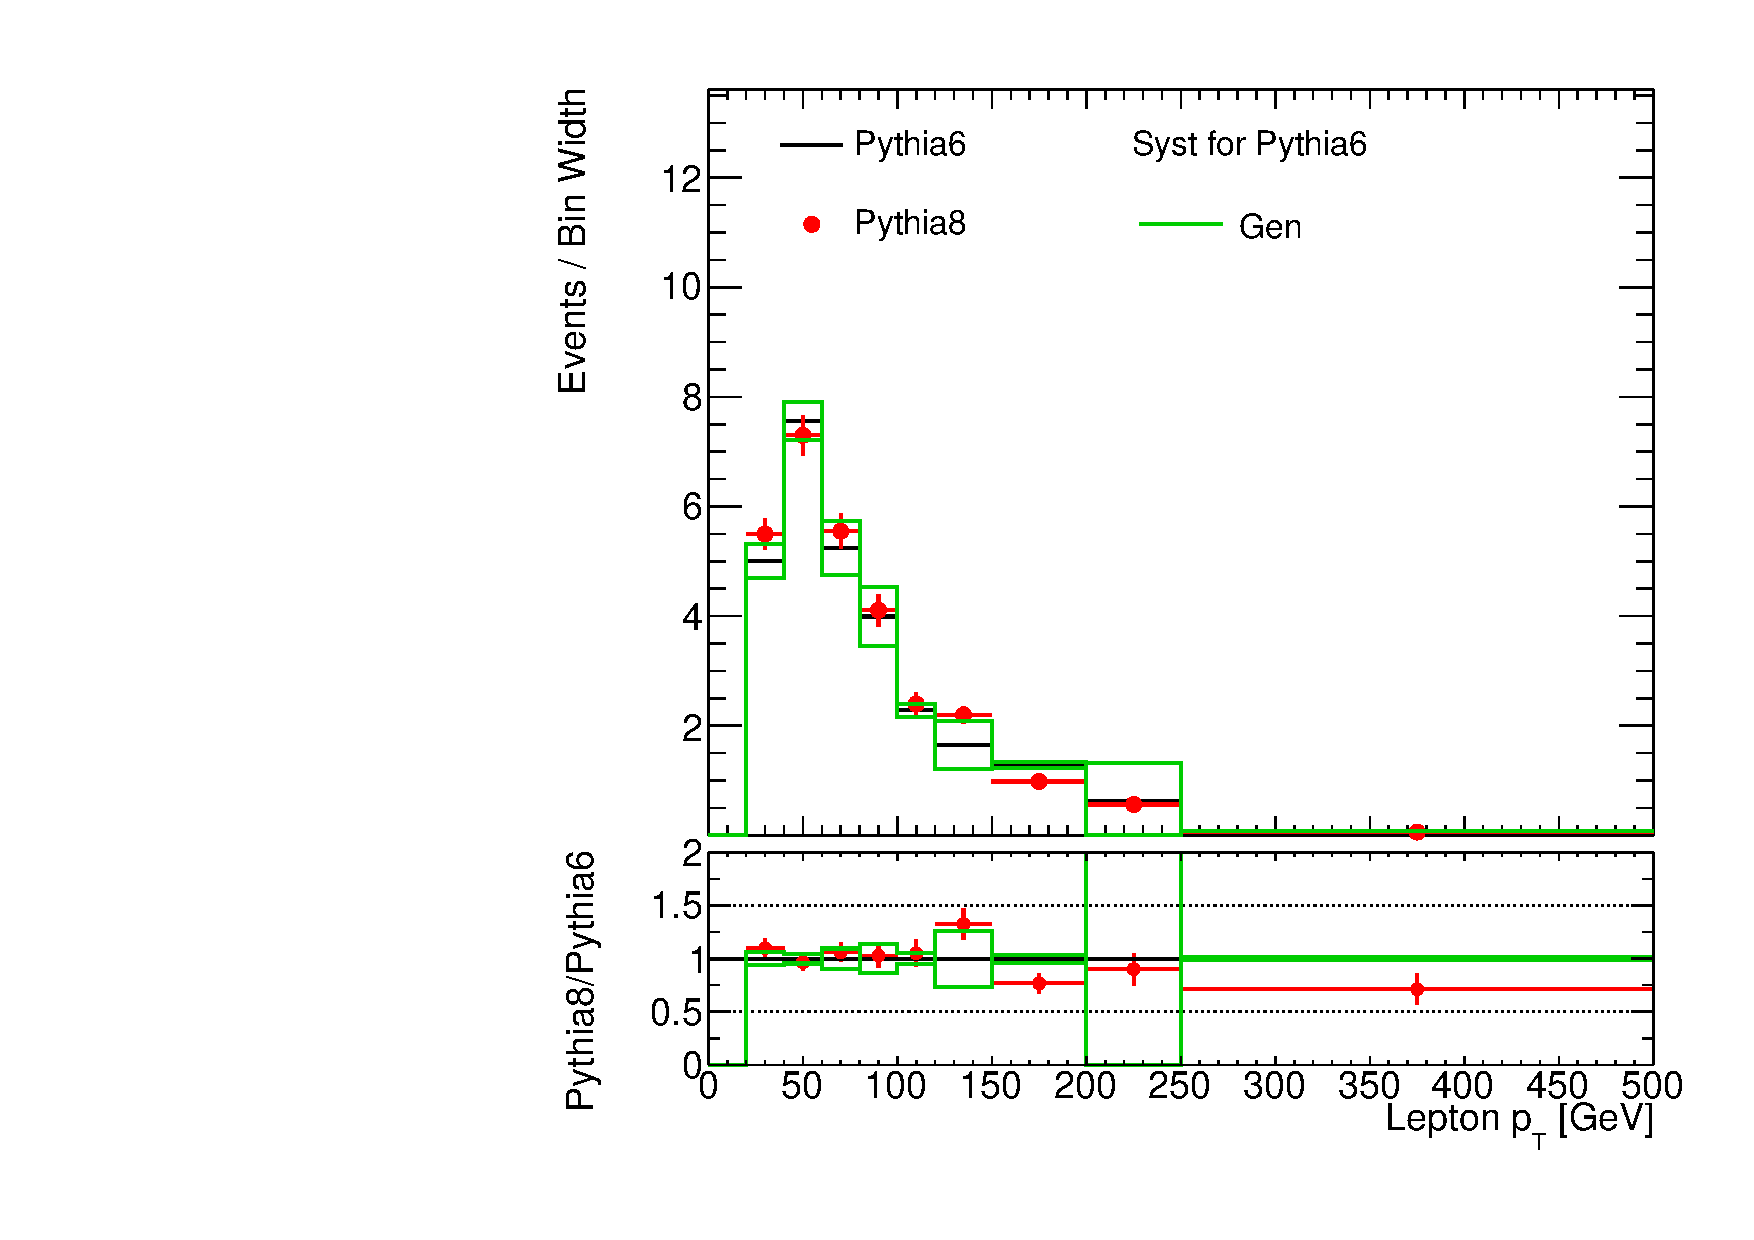
\includegraphics[scale=0.33]{./figures/boosted/TTBarPy6VsPy8/TTBarPy6VsPy8_SR_LepPt_gen}    
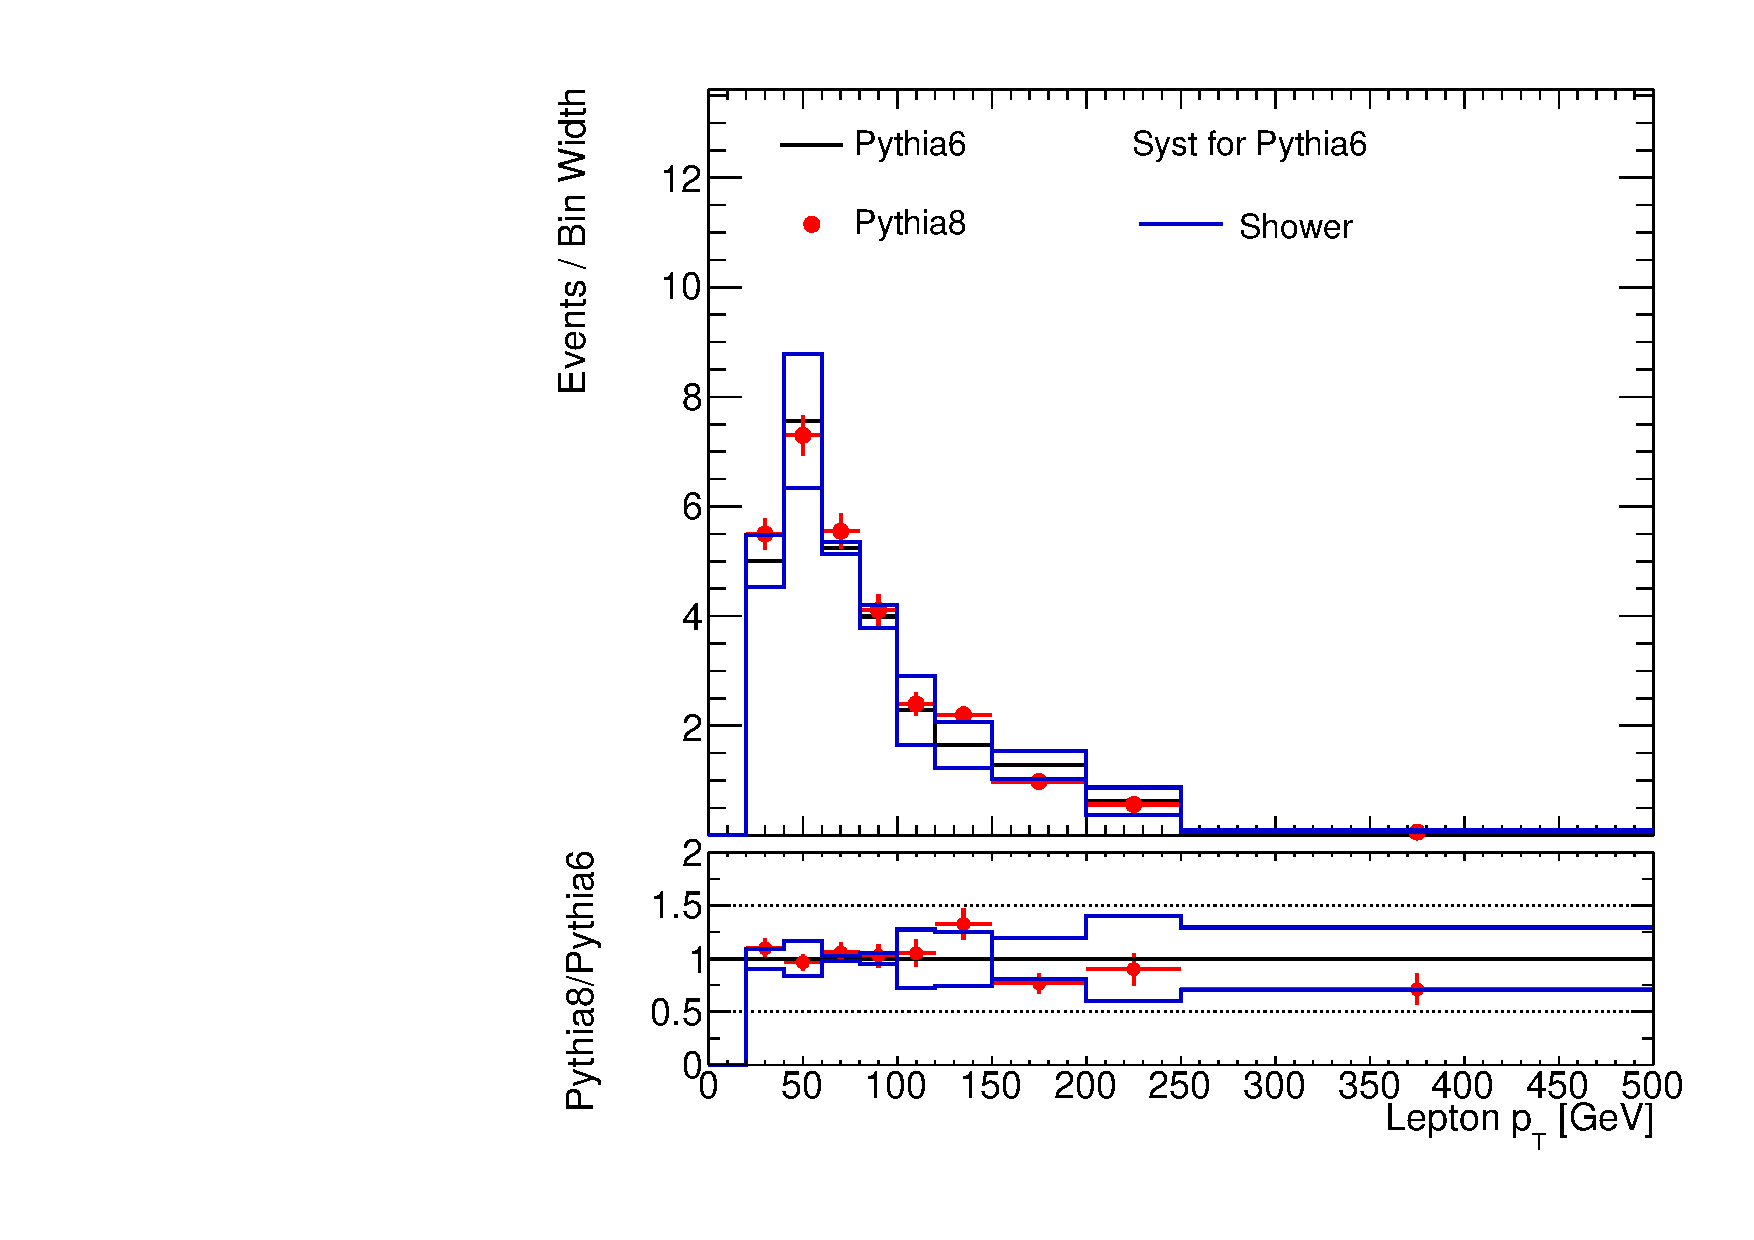
\includegraphics[scale=0.33]{./figures/boosted/TTBarPy6VsPy8/TTBarPy6VsPy8_SR_LepPt_shower} \\
\par\medskip
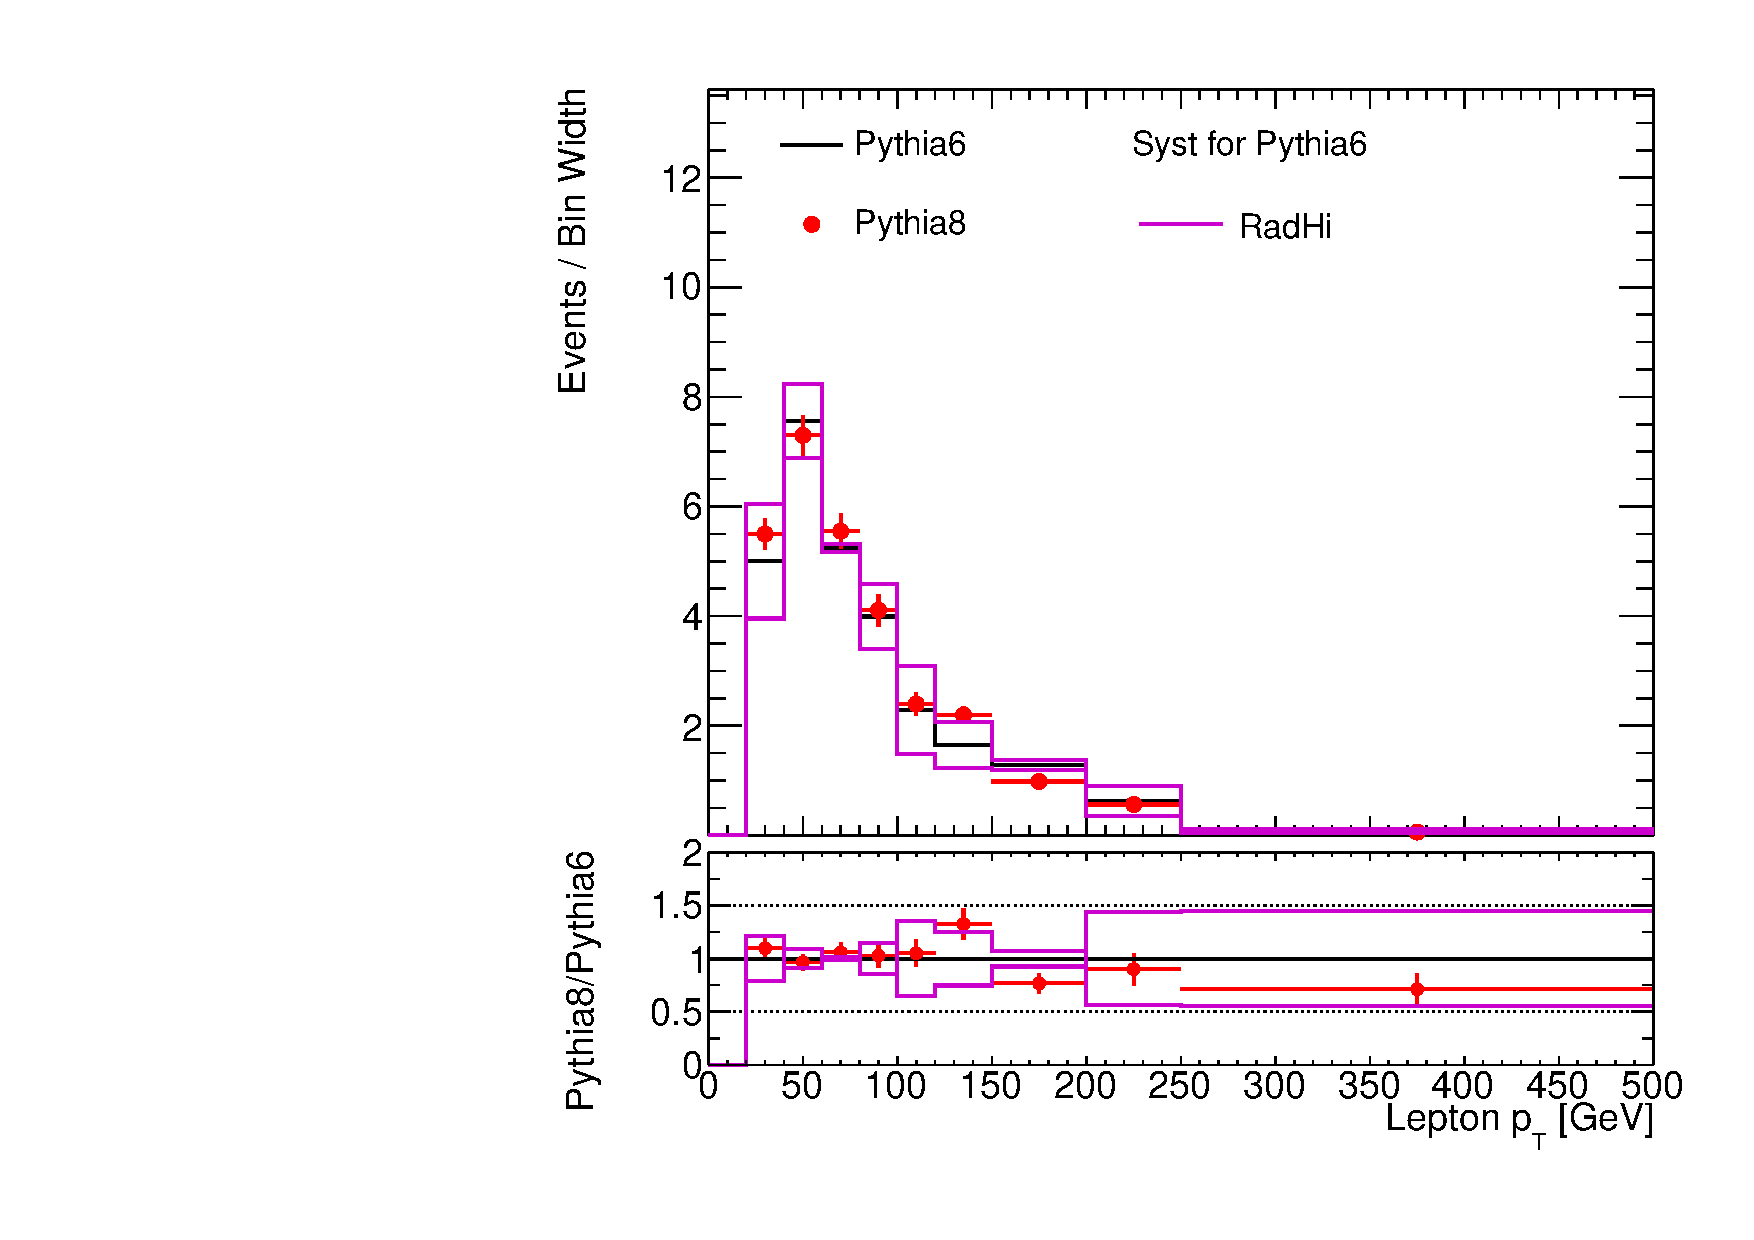
\includegraphics[scale=0.33]{./figures/boosted/TTBarPy6VsPy8/TTBarPy6VsPy8_SR_LepPt_radhi}
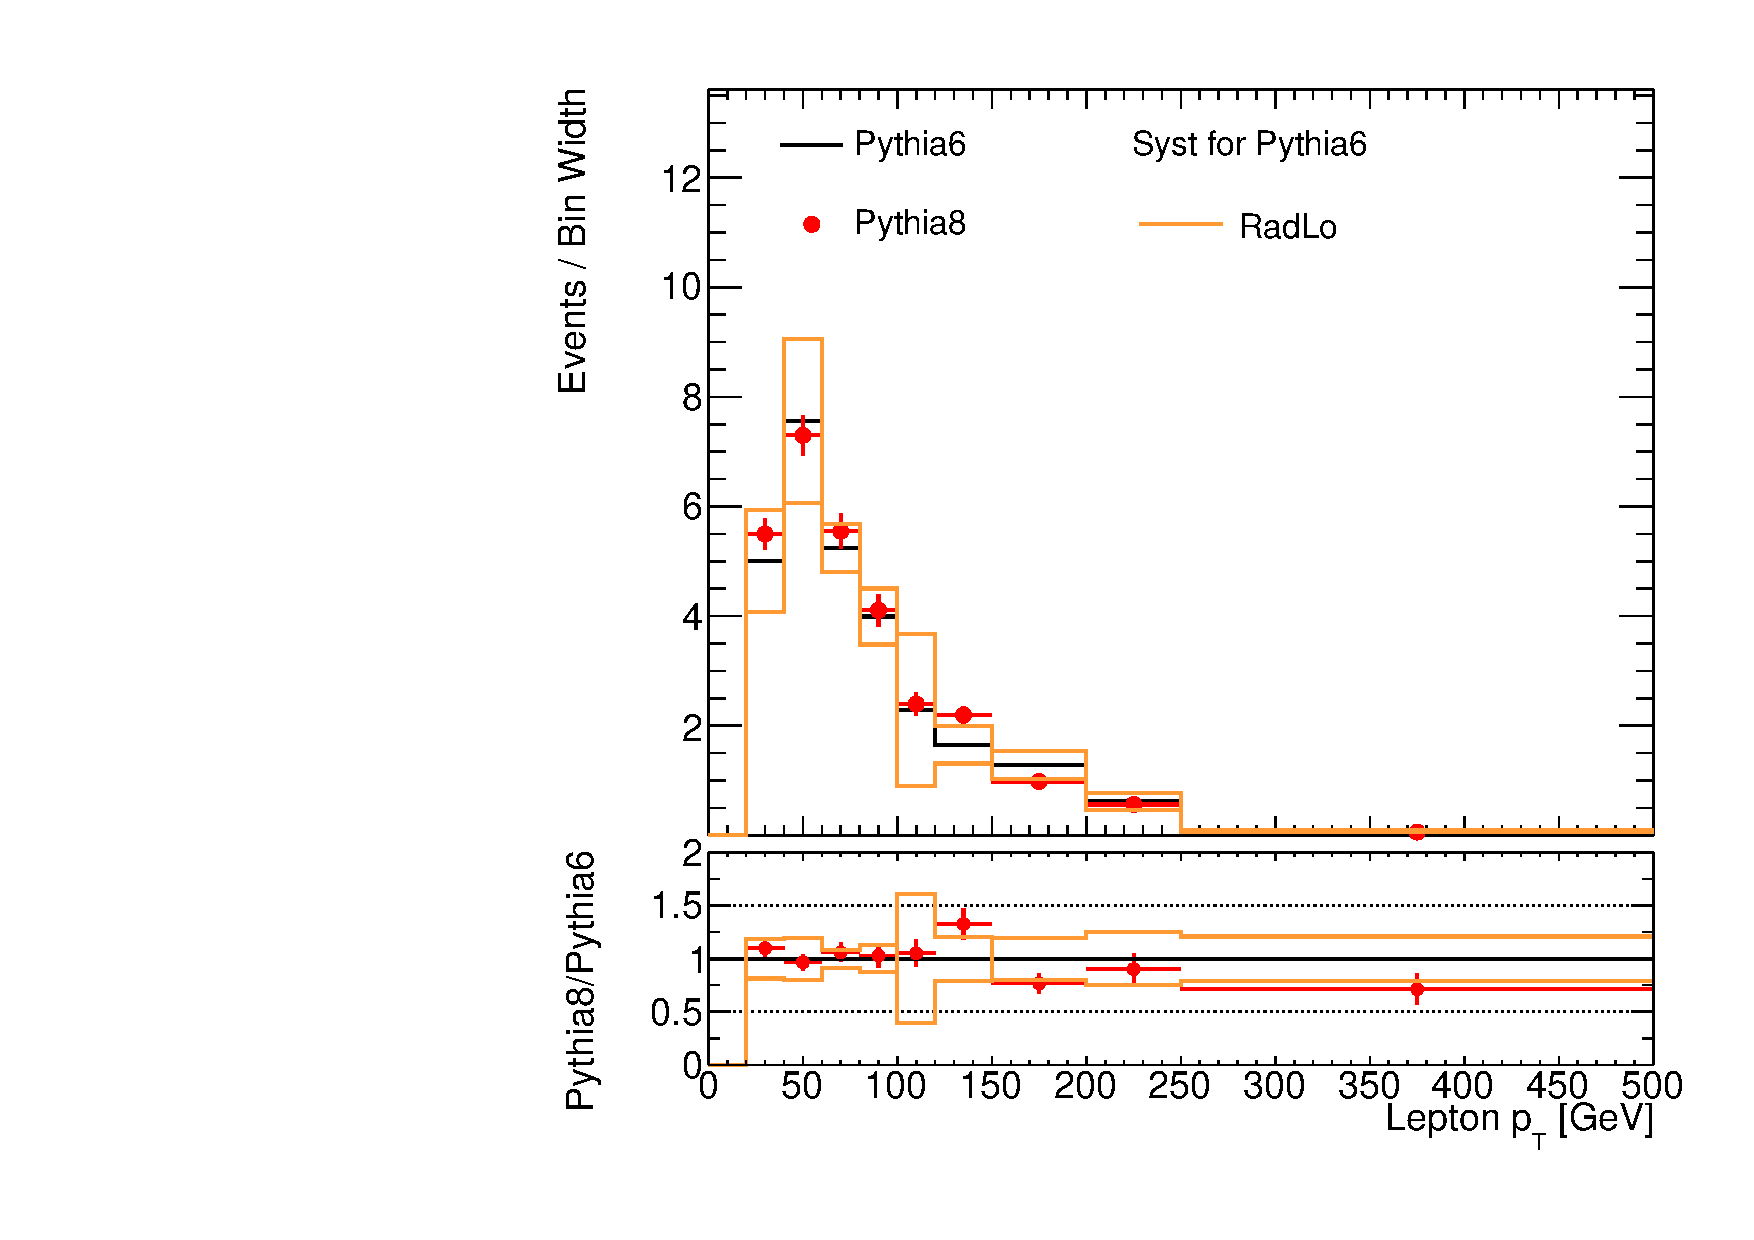
\includegraphics[scale=0.33]{./figures/boosted/TTBarPy6VsPy8/TTBarPy6VsPy8_SR_LepPt_radlo}
\caption{Lepton \pt distribution, in the 2-tag signal region, comparisons between Powheg+Pythia6 and Powheg+Pythia8 $t\bar{t}$ MC. 
The systematic variation for Powheg+Pythia6 is shown in each plot.}
\label{fig:boosted_ttbarpy6py8_LepPt}
\end{center}
\end{figure}


\begin{figure}[!h]
\begin{center}
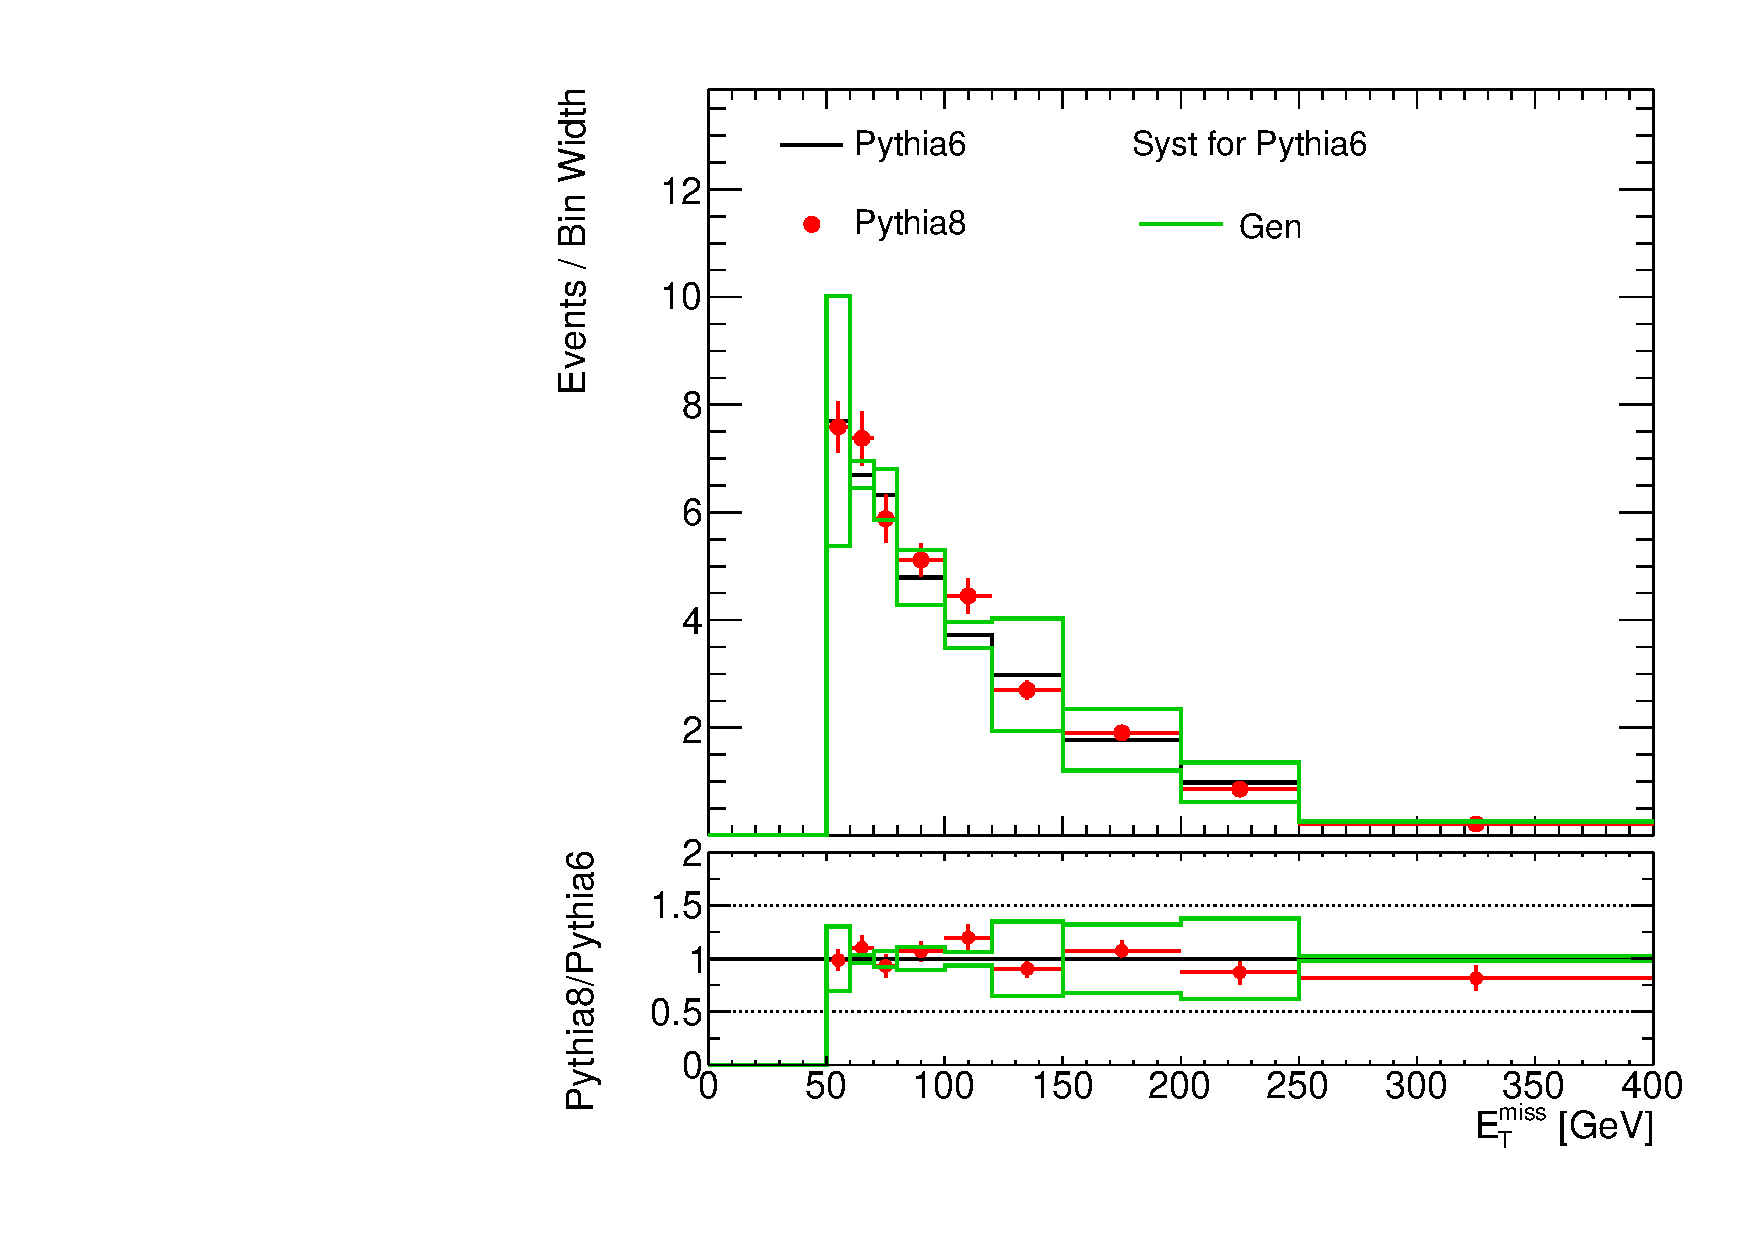
\includegraphics[scale=0.33]{./figures/boosted/TTBarPy6VsPy8/TTBarPy6VsPy8_SR_MET_gen}  
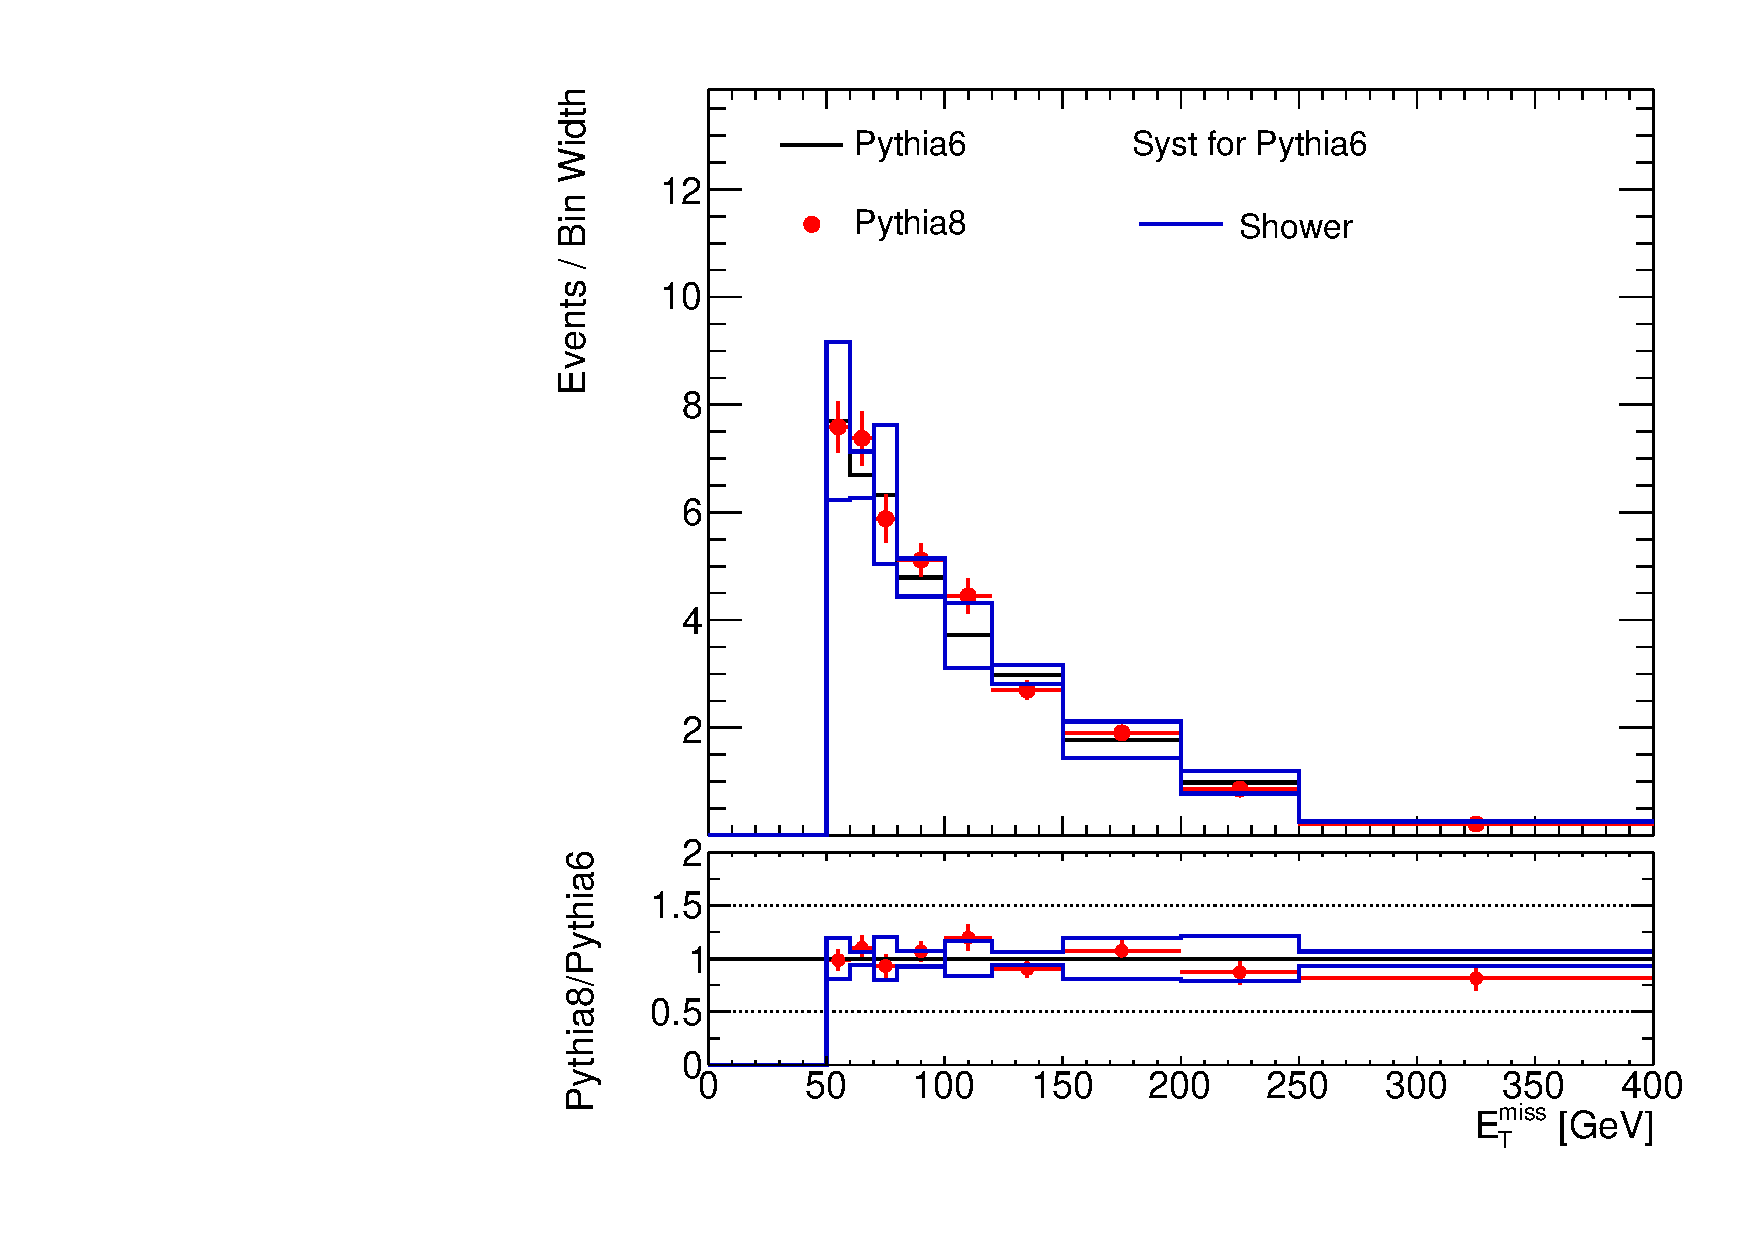
\includegraphics[scale=0.33]{./figures/boosted/TTBarPy6VsPy8/TTBarPy6VsPy8_SR_MET_shower} \\
\par\medskip
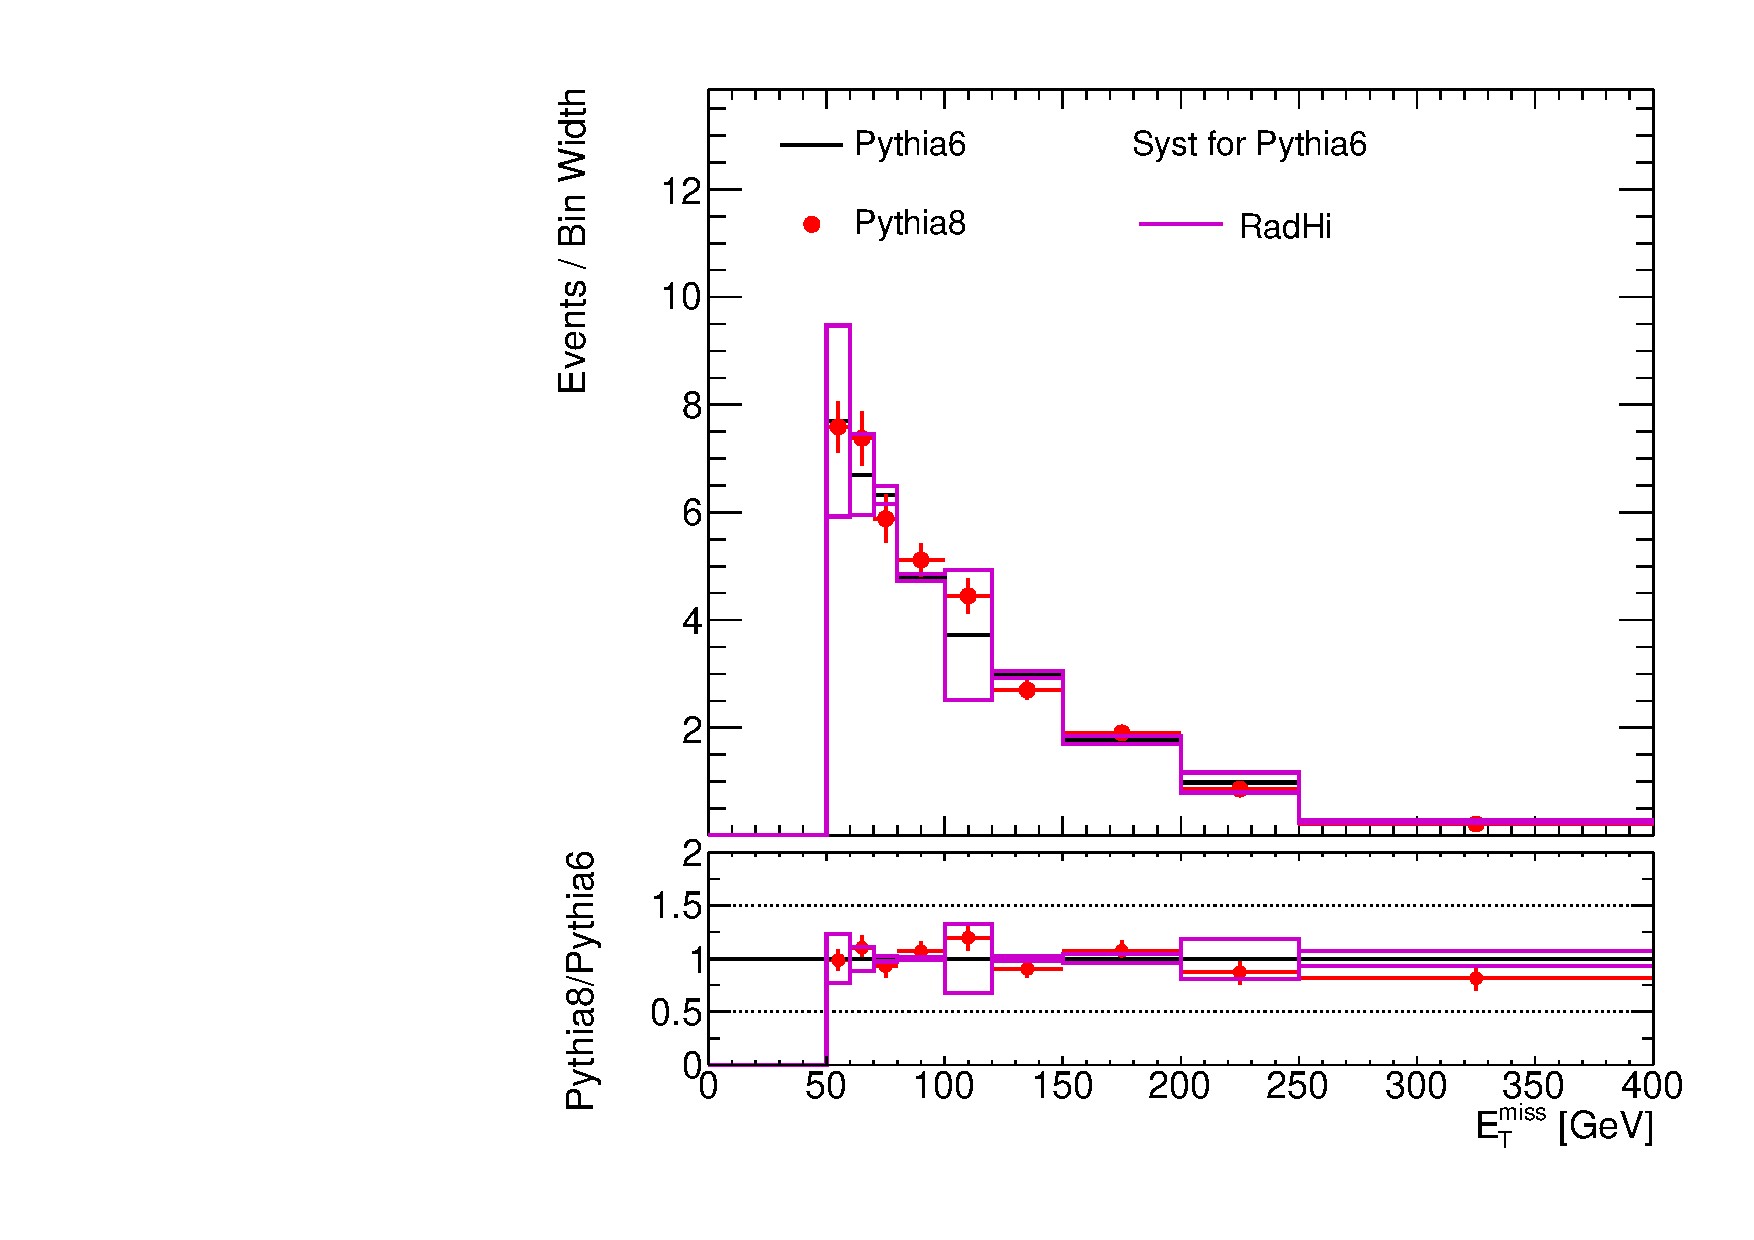
\includegraphics[scale=0.33]{./figures/boosted/TTBarPy6VsPy8/TTBarPy6VsPy8_SR_MET_radhi}
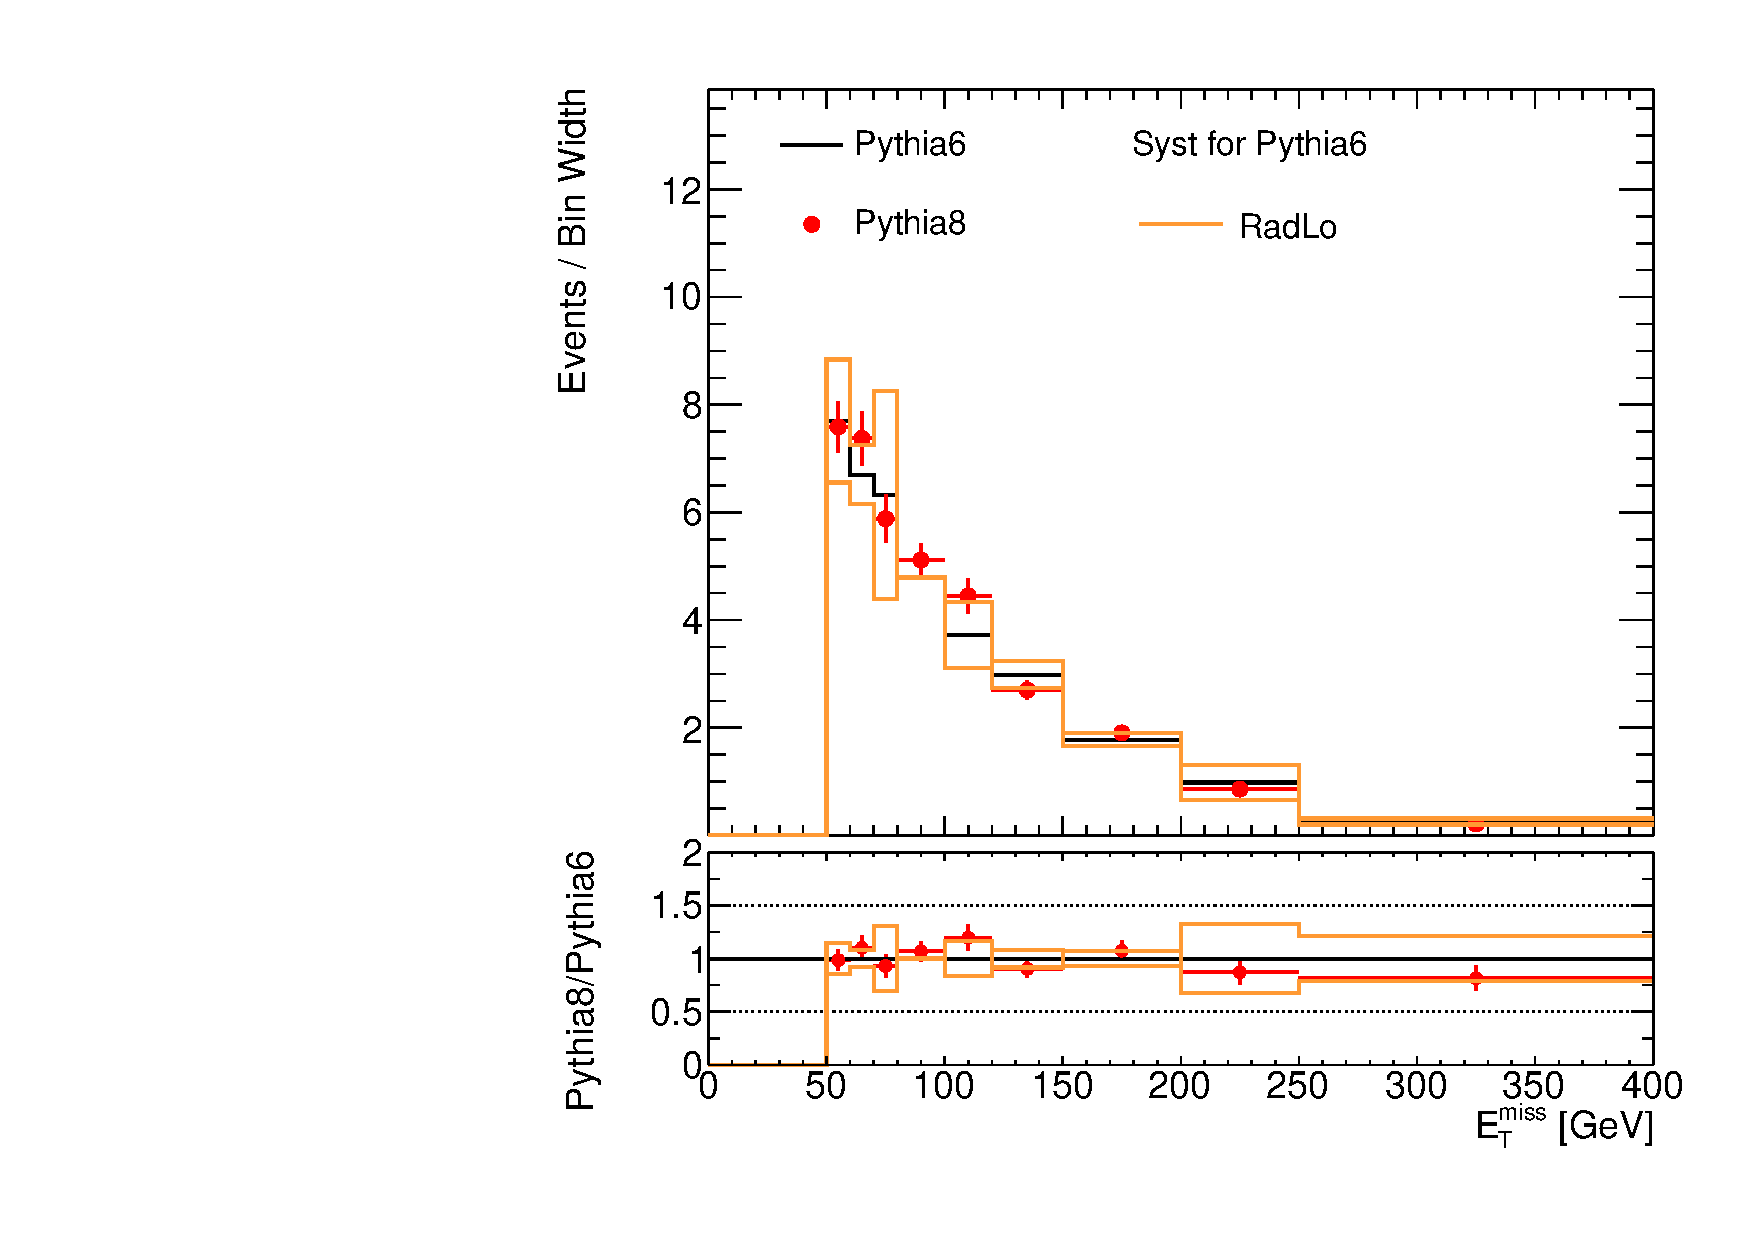
\includegraphics[scale=0.33]{./figures/boosted/TTBarPy6VsPy8/TTBarPy6VsPy8_SR_MET_radlo}
\caption{\met distribution, in the 2-tag signal region, comparisons between Powheg+Pythia6 and Powheg+Pythia8 $t\bar{t}$ MC. 
The systematic variation for Powheg+Pythia6 is shown in each plot.}
\label{fig:boosted_ttbarpy6py8_MET}
\end{center}
\end{figure}

\begin{figure}[!h]
\begin{center}
\includegraphics[scale=0.33]{./figures/boosted/TTBarPy6VsPy8/TTBarPy6VsPy8_SR_WlepMtATLAS_gen} 
\includegraphics[scale=0.33]{./figures/boosted/TTBarPy6VsPy8/TTBarPy6VsPy8_SR_WlepMtATLAS_shower} \\
\par\medskip
\includegraphics[scale=0.33]{./figures/boosted/TTBarPy6VsPy8/TTBarPy6VsPy8_SR_WlepMtATLAS_radhi}
\includegraphics[scale=0.33]{./figures/boosted/TTBarPy6VsPy8/TTBarPy6VsPy8_SR_WlepMtATLAS_radlo}
\caption{Transverse mass of lepton and \met  distribution, in the 2-tag signal region, comparisons between Powheg+Pythia6 and Powheg+Pythia8 $t\bar{t}$ MC. 
The systematic variation for Powheg+Pythia6 is shown in each plot.}
\label{fig:boosted_ttbarpy6py8_WlepMtATLAS}
\end{center}
\end{figure}




